

\documentclass[doctor]{thesis}



\usepackage[cmex10]{amsmath}
\usepackage{amsthm,amssymb}
\usepackage{flafter}
\usepackage[pdftex]{graphicx} \graphicspath{{./figures/}} 
\DeclareGraphicsExtensions{.pdf,.png,.jpg}

%\usepackage[caption=false]{subfig}

\usepackage{booktabs}

\usepackage{url}
\urlstyle{same} 

% \title{Resource constrained genomics via succinct data structures: Complex variants exposed as features in massive sample sets for sample origin classification}

\title{Enhancing Space and Time Efficiency of Genomics in Practice Through Sophisticated Applications of the FM-Index}

\author{Martin D. Muggli}

\email{martin.muggli@colostate.edu}

\department{Department of Computer Science}

\semester{Fall 2018}

\advisor{Ross McConnell}
%\coadvisor{Co-Advisor Name}
\committee{Charles Anderson}
\committee{Hamid Chitsaz}
\committee{Paul S Morley}

% This document contains text and art co-authored with others and whose copyright has been assigned to Springer or Oxford University Press.  It is reproduced with permission. All other content, 
\mycopyright{Copyright by Martin D. Muggli 2018 \\
All Rights Reserved
}
% both all other co-authors and  from  copyright holders in compliance with university requirements allowing non-original work.  

\abstract{Genomic sequence data has become so easy to get that the computation to process it has become a bottleneck in the advancement of biological science.  A data structure known as the FM-Index both compresses data and allows efficient querying, thus can be used to implement more efficient processing methods.  In this work we apply advanced formulations of the FM-Index to existing problems and show our methods exceed the performance of competing tools.   }

% \abstract{  Modern genome sequencing is largely based on a process of randomly breaking replicated copies of a genome into fragments, using various technologies to capture the nucleotide sequence within these fragments (resulting in strings known as reads), and then using assembly software to attempt to reconstruct the original genome sequence from the reads.
% This process is challenging as genomes contain repeated regions, and repeated regions much longer than read length confound assemblers, limiting their ability to completely and correctly reconstruct genomes successfully.
% Correct and complete genome assembly is important because genomes encode elements that cooperate with others in close proximity, and thus not just the content, but  genome structure has important biological implications.
% To the extent quality automated genome reconstruction is possible, there is an additional challenge of accessibility, as some of the most successful assembly software requires unusually high-end servers or clusters.
% This limits their usefulness to biologists with access and skill to use such machines and hence more efficient computational techniques are of value.
% Beyond efficiency and correctness of algorithms, there is interplay between computational approach, sequencing technology (which vary in read length, accuracy, applicability, and level of detail), and the assembly quality that may result.
% In this report, we will expand on the concepts introduced here and review a selection of modern computational assembly tools, the sequence data on which they operate, and discuss important advantages, limitations, and possible extensions of them as well as their relationship to each other in the context of the sequence assembly problem.
% }


\acknowledgements{I would like to thank Christina Boucher who filled the roll of advisor for all of this work for her patience, guidance, and insight in my training. I would also like to thank my committee, Ross McConnell, Charles Anderson, Hamid Chitsaz, and Paul S Morley, for their continued help and support. I would like to thank the many people who have supported me emotionally throughout this work, specifically: Alex Bowe, Lindsay Burchfield, Aaron Ciuffo, Katie Davidson, Teri Dillion, Thomas Harrison, Amber Johnson, Anne Mangiardi, Piper Murray, Simon Puglisi, Susan Rainey, Sanjay Rajopadhye, Sara Rector, Stacey Reynolds, Basir Shariat, Mike Storlie, Michelle Strout, John Wagner, Jason Walp, Adrienne Watral and others who I may have forgotten.  I would also like to thank the various people and organizations  whose outstanding science work provided inspiration: Richard P Feynman, ESA, CERN, LIGO, GHC. In addition, I would like to thank my co-authors for their contribution to our work. And last but not least I would like to thank my family, Jaynie Muggli, Jim Muggli, and Karen Muggli for their support as well.
}


\usepackage[pdfpagelabels,pdfusetitle,colorlinks=false,pdfborder={0 0 0}]{hyperref}

\usepackage{graphicx}
\usepackage{sidecap}
\usepackage{algorithm}
\usepackage{algorithmicx}
\usepackage[noend]{algpseudocode}
\usepackage{multirow}
\usepackage{pbox}
\usepackage{subcaption}
\def\twin{\mbox{\rm \textsc{Twin}}}
\def\ST{\mbox{\rm {\sf ST}}}
\def\SA{\mbox{\rm {\sf SA}}}
\def\ISA{\mbox{\rm {\sf ISA}}}
\def\LZ{\mbox{\rm {\sf LZ}}}
\def\LF{\mbox{\rm {\sf LF}}}
\def\FMI{\mbox{\rm {\sf FMI}}}
\def\FM{\mbox{\rm {\sf FM}}}
\def\rank{\textsf{rank}}
\def\pathlabel{\mbox{\rm {\sf pathlabel}}}
\def\lcp{\mbox{\rm {\sf lcp}}}
\def\rmq{\mbox{\rm {\sf rmq}}}
\def\x{\mbox{\rm {\sf x}}}
\def\X{\mathsf{X}}
\def\MS{\mbox{\rm {\sf MS}}}
\def\B{\mathsf{B}}
\def\ssB{\mbox{\rm {\sf {\scriptsize B}}}}
\def\A{\mathsf{A}}
\def\Pr{\mbox{\rm {\sf P}}}
\def\R{\mbox{\rm {\sf R}}}
\def\Y{\mbox{\rm {\sf Y}}}
\def\Y{\mathsf{Y}}
\def\ssY{\mbox{\rm {\sf {\scriptsize Y}}}}
\def\Z{\mathsf{Z}}
\def\C{\mbox{\rm {\sf C}}}
\def\D{\mbox{\rm {\sf D}}}
\def\M{\mbox{\rm {\sf M}}}
\def\F{\mbox{\rm {\sf F}}}
\def\BWT{\mbox{\rm {\sf BWT}}}
\def\ABWT{\mbox{\rm {\sf ABWT}}}
\def\L{\mbox{\rm {\sf L}}}
\def\dollar{\$}
\def\citep{\cite}
 \def\I{\mbox{\rm {\sf I}}}
 \def\O{\mbox{\rm {\sf O}}}
\DeclareRobustCommand{\bigO}{\text{\usefont{OMS}{cmsy}{m}{n}O}}
\def\sequel{\mbox{\rm \textsc{misSEQuel}}}
\def\suffix{\mbox{\rm {\sf suffix}}}
\def\prefix{\mbox{\rm {\sf prefix}}}
\def\select{\textsf{select}}
\def\dopp{\mbox{\rm \textsc{Kohdista}}}
\newcommand{\Oh}[1]
	{\ensuremath{\mathcal{O}\!\left({#1}\right)}}
\newcommand{\access}
	{\ensuremath{\mathsf{access}}}
\newcommand{\occ}
	{\ensuremath{\mathsf{occ}}}
\newcommand{\nodelabel}
	{\ensuremath{\mathsf{label}}}
\newcommand{\Psiop}
	{\ensuremath{\mathsf{\Psi}}}
\newcommand{\mus}[1]
	{\SI{#1}{\micro\second}}
\newcommand{\elabel}{\ensuremath{\mathsf{label}}}
\newcommand{\EBWT}{\ensuremath{\mathsf{EBWT}}}
\def\flags{\mbox{\rm {\sf flags}}}
\def\BF{\mbox{\rm {\sf BF}}}
\def\BL{\mbox{\rm {\sf BL}}}
\def\vari{\mbox{\rm {\sc Vari}}}
\def\merge{\mbox{\rm {\sc Merge}}}
\def\ours{\mbox{\rm {\sc VariMerge}}}
\def\ours{\mbox{\rm \textsc{Vari}}}
\def\vari{\mbox{\rm {\sc Vari}}}
\def\merge{\mbox{\rm {\sc Merge}}}
\def\ours{\mbox{\rm {\sc VariMerge}}}
\newtheorem{observation}{Observation}
\newtheorem{theorem}{Theorem}

\begin{document} 
\frontmatter 
\maketitle
\makemycopyright
\makeabstract
\makeacknowledgements   
% \prelimtocentry{Dedication} \begin{flatcenter} 
%         DEDICATION

%         \vfill 
% %    \noindent \textit{I would like to dedicate this thesis to my dog fluffy.}
%     \vfill \end{flatcenter}
\newpage

\tableofcontents
%\listoftables       \listoffigures      
\mainmatter 







































\chapter{Introduction}
\bigskip

With the advent of high throughput sequencing, biologists have gained access to massive amounts of data sampled from their specimens.  While this is a boon for biologists, all this data must be processed to yield useful information and many times, state of the art computing hardware and software are a limiting factors for biological inquiry.  For example, a set of samples from 3,765 \emph{E. coli} would require over 3 TB of memory to represent in a state of the art tool, far exceeding even the 1 TB of RAM in machines some labs are fortunate to have access to.

There are however opportunities for improvement.  Existing methods store their data, which usually has some inherent redundancy, in a direct, one-to-one representation. Thus enhancing these methods with compression techniques can reduce their memory footprint.  Additionally, data often contain erroneous values which existing methods accomodate with some form of exhaustive search techniques.  Instead, sufficiently powerful indexing techniques can provide error tolerant lookup mechanisms instead and reduce the runtime.

A data structure known as the FM-Index can provide both indexing and compression simultaneously.   In fact, the basic string search and compression capabilities of the FM-Index are fairly well known and applied.  The search capabilities are used within the nearly ubiquitous BWA~\cite{bwa} software in bioinformatics.  And the compression capabilities underlying the FM-Index are even more widespread in tools such as the BZIP2.

The FM-Index, however, is not a drop in replacement for existing techniques. Various problems need more than simple string indexing over small alphabets, but require indexing graphs and large alphabets.  Fortunately, there are more advanced developments that make the FM-Index applicable to graphs and queries based on ordinal elements.

We explore extending the reach of the available tool set with new tools which apply sophisticated forms of the FM-Index.  This enhances the efficiency on each of the runtime and space requirements over state of the art tools on existing genomics problems.  
%TODO: keep this below???
%Furthermore, we can then use these to aid in generating new results which would previously have been more expensive or impossible to produce, thus illustrating that these enhancements are useful in practice. 
Specifically to illustrate this, we enable detection of variants among a dataset of approximately 16,000 \emph{Salmonella} samples taken from food production facilities.  Additionally, we demonstrate the usefulness of tools which reduce runtime by means of sophisticated indexing on a more recent form of genomic data in the form of optically derived restriction maps.



\section{Background}

Within the scope of genomics, there are two overarching tasks we'll focus on improving: The acquisition of complete genome sequences for organisms and detection of variations of genomes among a population.

Though scientists have been advancing the lab methods for sequencing genomes for almost four decades, no method today can sequence entire chromosomes. Genomic DNA still must  be sheared into fragments small enough for available technology to sequence (currently approx 100-10,000 base pairs), and then an assembly process used to reconstruct the original genome sequence by joining related fragments' strings (called \emph{reads}) based on their similar substrings \cite{nagarajan2013sequence,staden1980new}.

The question naturally arises for how we can find these similar regions between reads, especially in the presence of noise such as read errors.
An alignment is a relationship between two strings which may not exactly match each other.  As such, alignments are an effective measure of similarity\cite{needleman1970general}.  While alignments have many applications, we will first focus our discussion on alignments as relationships between strings (e.g., genomic data such as reads, the genome itself, or other sequence data derived from the genome).
An alignment can be expressed as a sequence of edits (insertions, deletions, and substitutions) to convert one string into another.  When we align genomic data, these edits appear either in the presence of read errors when the two strings originated as reads of a single genome, or in the presence of variation between two genomes otherwise.
Scores are often associated with alignments based on the sum of scores of the edit operations which compose alignments. A good scoring alignment between two strings can serve as an indicator that they may share a common genomic origin.

Often the scoring scheme allows penalty free runs of insertions or deletions at one or more ends of a sequence, allowing for the fact that two strings may both cover a shared region of a genome but each string also covering a portion the other did not.
If opposing ends of the two sequences are allowed not to match in a penalty free manner, it is called semi-global alignment and is the expected case for two reads that overlap the same locus but have different start and end positions.

Dynamic programming based algorithms can be used to find the optimal alignment between two strings under some scoring scheme; however, this is typically formulated as an $\bigO(mn)$ problem where $m$ and $n$ are the lengths of the strings. While this running time is not necessarily a problem between a single pair of strings, we're often interested in all high scoring alignments between all pairs of strings.  Computing this would entail running dynamic programming $O(|R|^2)$ times where $R$ is the set of all reads, making the composition of these running times far too time consuming for all but the smallest genomes. Thus other methods we'll explore later often replace dynamic programming based alignment techniques.

When the objective is to recover a complete genome sequence given a set of reads, it is necessary to find similar regions between reads such that we can reconstruct the genomic regions where the reads originate.  There are two paradigms in active use for this: overlap-layout-consensus based and de Bruijn graph based.

Overlap layout consensus assembly works by finding alignments between pairs of reads, representing those alignments in a graph where reads form nodes and alignments form edges, and then finding Hamiltonian tours \cite{myers1995toward}.

De Bruijn graph based assemblers chop reads up into a series of overlapping substrings of length $k$ called $k$-mers \cite{pevzner2001eulerian}.
$k$-mers are subdivided into a $(k-1)$-mer prefix and $(k-1)$-mer suffix.
Each $(k-1)$-mer becomes a node in a graph, with the original $k$-mer becoming a directed edge connecting them.  
All vertices with the same $(k-1)$-mer label are then glued together. When vertices with the same $(k-1)$-mer label originate from different reads, the glued node is how a similar region between those reads is represented. Thus gluing $(k-1)$-mers takes the place of finding alignments between reads.  This graph is then traversed, finding Eularian tours.

In the ideal case, either method could reconstruct a genome from reads given enough resources.  However, this task is complicated in practice by the fact that genomes contain repeated regions. This means that two reads that appear to share a similar substring may actually have been read from different loci (or locations) in the genome.  Thus for either assembly approach, repeats in the genome cause read data originating from disparate loci to have a spurious relation in an assembly graph (either glued together, becoming one node in the de Bruijn graph, or having an alignment edge in the overlap-layout-consensus graph). These coincidental alignment relations introduce cycles in the graph.  Such cycles can make it impossible to unambiguously determine how to reconstruct the original genome - while the original genome sequence can be found as one specific walk through either graph, it's typically not possible to determine which of many possible walks in an assembly graph represents the true genome path, so assembly tools emit those non-branching paths which can be inferred with high confidence to be contiguous regions of the genome.
These paths spell strings known as \emph{contigs}.

\subsection{FM-Index}

As mentioned previously, finding alignments by means of pairwise dynamic programming can be too computationally expensive for all but the smallest genomes.  However, with relatively error-free strings (either because an error correction procedure has been run, or the strings are small enough to often avoid errors, or the sequencing technology is highly accurate) another alternative to dynamic programming based alignment is to use a data structure called a \emph{suffix array} for finding predominantly identical common substrings.
Conceptually, this is an array consisting of all the suffixes of a string in sorted order \cite{manber1993suffix}.
Associated with each element in the array is the index in the original string where that element's suffix begins.
This can be efficiently implemented in practice. For example, in the C programming language, the suffix array can be represented as an array of either pointers or offsets into the original string, avoiding the redundancy of storing each suffix separately. 
Any string that matches the prefix of some suffix of the original string of length $n$ can then be found by binary search in time $\bigO(\log n)$.

Formally,  we consider a string $\X = \X[1..n] = \X[1]\X[2]\ldots
\X[n]$ of $|\X| = n$ symbols drawn from the alphabet $\Sigma =[0..\sigma-1]$.
For $i=1,\ldots,n$ we
write $\X[i..n]$ to denote the \emph{suffix} of $\X$ of length $n-i+1$,
that is $\X[i..n] = \X[i]\X[i+1]\ldots \X[n]$.
Similarly, we write
$\X[1..i]$ to denote the \emph{prefix} of $\X$ of length $i$.
$\X[i..j]$ is the \emph{substring} $\X[i]\X[i+1]\ldots \X[j]$ of $\X$
that starts at position $i$ and ends at $j$.

\subsubsection{Suffix arrays and suffix array intervals.}
\label{backward-search}
The suffix array~\cite{mm1993} $\SA_{\X}$ (we drop subscripts when
they are clear
from the context) of a string $\X$
is an array $\SA[1..n]$ which
contains a permutation of the integers $[1..n]$ such that $\X[\SA[1]..n]
\prec \X[\SA[2]..n] \prec \cdots \prec \X[\SA[n]..n]$.  In other words, $\SA[j] =
i$ if and only if $\X[i..n]$ is the $j^{\mbox{{\scriptsize th}}}$ suffix of $\X$
in lexicographical order. Here, $\prec$ denotes lexicographic precedence.





A clever data structure known as an \emph{FM-index} is often used as a memory efficient alternative to a suffix array.
To explain this structure, we will start with a conceptual model.
The source string has a special out-of-alphabet symbol (e.g., `\$') appended to it.
Then all possible rotations of this string are created and stacked vertically as rows in a matrix.
The rows of this matrix are then sorted, yielding a matrix similar to the suffix array.
The string comprising the last column of this matrix is  known as the Burrows-Wheeler transform ($\BWT$)~\cite{burrows1994block} of the source string.

Formally, for a string $\X$, let $\F$ be the list of $\X$'s characters sorted lexicographically by the suffixes starting at those characters, and $\L$ be the list of $\X$'s characters sorted lexicographically by the suffixes starting immediately after those characters.  (The names $\F$ and $\L$ are standard for these lists.)  If \(\Y [i]\) is in position $p$ in $\F$ then \(\Y [i - 1]\) is in position $p$ in $\L$.  Moreover, if \(\Y [i] = \Y [j]\) then \(\Y [i]\) and \(\Y [j]\) have the same relative order in both lists; otherwise, their relative order in $\F$ is the same as their lexicographic order.  This means that if \(\Y [i]\) is in position $p$ in $\L$ then (assuming arrays are indexed from 0) in $\F$ it is in position
\[|\{h\,:\,\Y [h] \prec \Y[i]\}| + |\{h\,:\, \L [h] = \Y [i],\ h \leq p\}| - 1\,.\] Finally, notice that the last character in $\X$ always appears first in $\L$.  It follows that we can recover $\X$ from $\L$, and thus $\L$ is the famous {\em Burrows-Wheeler Transform (BWT)}~\cite{bw1994} of $\X$.  For an example string ``catgcat\$'', the Burrows-Wheeler transform is ``tccg\$taa''.

%TODO CHUCK asked for a very small example
More succinctly, the Burrows-Wheeler Transform~\cite{bw1994} $\BWT[1..n]$ is a
permutation of $\X$ such that $\BWT[i] = \X[\SA[i]-1]$ if $\SA[i]>1$
and $\$$ otherwise.



The $\BWT$ has a number of useful properties.
If the source string has repeats, then the sorted rotations will naturally position all the repeated suffixes sharing the same prefix in a contiguous run of rows.
All of those same suffixes without their first character will also be in a contiguous run of rows, and since each row is a rotation, all the first characters we considered initially will be found in the last column as a run of the repeated character.
Runs of repeated characters can be compressed by various means, such as run length encoding where the repeated character and the length of the run are stored instead of the repeated instances of that character. Thus, the BWT  of a string containing repeats can be represented in less memory than the original string.
% Furthermore, the original string can be recovered from the BWT transform.

Note that in practice, the conceptual BWT matrix outlined above does not need to be constructed to get the BWT of the text; one can simply sort all the suffixes and take the character that precedes each suffix. This sequence of characters is then equivalent to the last column of our conceptual model since they are rotations in the matrix.

Additionally, by adding two auxiliary data structures (\emph{Occ}: a rank() capable dictionary for the last matrix column $L$ and \emph{S}\footnote{This is traditionally represented as $C$}: a trivial select() capable data structure for the equivalent of the first matrix column $F$) to the BWT, an extended data structure known as the aformentioned FM-index can be constructed. It can allow the BWT to act as a self index into the original string which allows exact matches to a query string to be found in time linear in the length of the query \cite{ferragina2000opportunistic}.  This works by finding a succession of intervals in the suffix array (whose elements correspond to those of the BWT as seen from the Burrows Wheeler matrix) which match progressively longer suffixes of a query string.



Formally, for a string $\Y$, the $\Y$-interval in the suffix array $\SA_{\X}$ is
the interval $\SA[s..e]$ that contains all suffixes having $\Y$ as a
prefix. The $\Y$-interval is a representation of the occurrences of
$\Y$ in $\X$. For a character $c$ and a string $\Y$, the computation
of $c\Y$-interval from $\Y$-interval is called a \emph{left extension}.





%Ferragina and Manzini~\cite{fm2005} linked $\BWT$ and $\SA$ in the
%following way.


Ferragina and Manzini~\cite{fm2005} first  realized BWT can be used for indexing in addition to compression.   Hence, if we know the range \(\BWT (\X) [i..j]\) is occupied by characters immediately preceding occurrences of a pattern $Y$ in $\X$, then we can compute the range \(\BWT (\X) [i'..j']\) occupied by characters immediately preceding occurrences of \(c Y\) in $\X$, for any character $c$, since
\begin{eqnarray*}
s' & = & |\{h\,:\,\X [h] \prec c\}| + |\{h\,:\,\X [h] = c, h < s\}| \\
e' & =  & |\{h\,:\,\X [h] \prec c\}| + |\{h\,:\, \X [h] = c, h \leq e\}| - 1\,.
\end{eqnarray*}
Notice \(e' - s' + 1\) is the number of occurrences of \(c Y\) in $S$.  The essential components of an FM-index for $\X$ are: (1) an array $S$ storing \(|\{h\,:\,\X [h] \prec c\}|\) for each character $c$ and, (2) a {\em rank} data structure $Occ$ for \(\BWT (\X)\) that quickly tells us how often any given character occurs up to any given position. To be able to locate the occurrences of a pattern $Y$ in $\X$ (in addition to just counting them), we can use a sampled suffix array of $\X$ and a bitvector indicating the positions in \(\BWT (\X)\) of the characters preceding the sampled suffixes.
%TODO include wavelet tree stuff here?

Hence, we define the function
$\rank_c(\X, i)$, for string $\X$, symbol $c$, and integer $i$, as
the number of occurrences of $c$ in $\X[1..i]$. Rank is used in {\em backward search}~\cite{fm2005} in order to compute left extension of a given string, i.e., the previous character.

To support rank queries in backward search, a data structure called a {\em wavelet tree} ~\cite{GNPtcs11}
can be used. It occupies $n\log\sigma + o(n\log\sigma)$
bits of space and supports $\rank$ queries in $\bigO(\log\sigma)$ time.
Wavelet trees also support a variety of more complex queries on the underlying string  efficiently~\cite{GNPtcs11}.
One such query we will use in this paper
is to return the set $Z$ of
distinct symbols occurring in $X[i,j]$, which takes
$\bigO(|Z|\log\sigma)$ time.


% TODO CHUCK wants a short section that summarizes remaining chapters
In the remainder of this text we will look at two broad problems in genomics.  In Chapter 2, we will examine approaches that are useful for validating draft genome assemblies.  In Chapter 3, we will examine methods for comparing genomes in large populations.  Finally, we'll conclude by considering the relationship between the graph based representation of genomic data that were presented.






\chapter{Reducing Runtime by Indexing}
\bigskip

In this section, we look at applications of the FM-Index which reduce alignment runtime over competing tools by using the indexing capabilities of sophisticated variations of the FM-Index.  In particular, we consider how an emerging form of genomic data, optically derived restriction maps, present special challenges but can still be aligned with the FM-Index.


\section[TWIN: Efficient Indexed Alignment of Contigs to Optical Maps]{TWIN: Efficient Indexed Alignment of Contigs to Optical Maps\protect\footnote{M. Muggli {\it et al.} Efficient indexed alignment of contigs to optical maps. In {\it Proceedings WABI}, pages 68-81, 2014.}}

In this section, we look at applying the FM-Index to aligning a consensus form of data, where the principle challenge to application is that we are dealing with sequences over a large alphabet and the symbols rarely match exactly. Later, we will build upon the solution explored here to solve alignment on raw, non-consensus data, which has additional complexities.
\subsection{Introduction}



In this section, we begin our more in depth investigation of succinct data structures.  Specifically, we examine how the FM-Index and wavelet tree can be used to store a compressed index of a string of integral valued symbols which can be efficiently queried. 
% We further show that this index based method not only increases the speed over dynamic programming methods, the faster speed enables other advancements to be investigated such as better assembly validation.

Our motivation for this application is as follows. Despite considerable research, \emph{de novo} genome assembly, the process of reconstructing long contiguous sequences (\emph{contigs}) from short sequence reads, still produces a substantial number of errors~\cite{sequel,Alkan:2011} and is easily misled by repetitive regions~\cite{salzberg}.

One way to improve the quality of assembly is to use secondary information (independent
of the short sequence reads themselves) about the order and orientation of contigs.   Optical mapping, which constructs ordered genome-wide high-resolution restriction maps, can provide such information. Optical mapping is a system that works as follows \cite{ORMenc,microfluidic}.  An ensemble of DNA molecules adhered to a charged glass plate are elongated by fluid flow.   An enzyme is then used to cleave them into fragments at loci where the enzyme's recognition sequence occurs. Next, the remaining fragments are highlighted with fluorescent dye and digitally photographed under a microscope. Finally, these images are analyzed to estimate the fragment sizes, producing a molecular map. Since the fragments stay relatively stationary during the aforementioned process, the images capture their relative order and size~\cite{Neely11}.   Multiple copies of the genome undergo this process, and a consensus map is formed that consists of an ordered sequence of fragment sizes, each indicating the approximate number of bases between occurrences of the recognition sequence in the genome \cite{Anantharaman01}.

The raw optical mapping data identified by the image processing is an ordered sequence of fragment lengths. Hence, an optical map with $m$ fragments can be denoted as $\ell = \{\ell_1, \ell_2, \ldots, \ell_m \}$, where $\ell_i$ is the length of the $i$th fragment in base pairs.  This  data can then be converted into a sequence of locations, each of which determines where a restriction site occurs.  We denote the converted data as follows: $L(x) = \{L_0 < L_1 < \cdots < L_n \}$, where $\ell_i = L_i - L_{i - 1}$ for $i = 1, \ldots, n$, and  $L_0$ and $L_n$ are defined by the original molecule as a segment of the whole genome by shearing. This latter representation is convenient for algorithmic descriptions. The approximate mean and standard deviation of the fragment size error rate for current consensus data \cite{error_rate} are zero and 150 bp, respectively.   See Figure~\ref{figure:fig1} for an illustration of the data produced by this technique. Each restriction enzyme recognizes a specific nucleotide sequence so a unique optical map results from each enzyme.%, and multiple enzymes can be used in combination to derive denser optical maps.
Optical maps have recently become commercially available for mammalian-sized genomes\footnote{OpGen (\url{http://www.opgen.com}) and BioNano (\url{http://www.bionanogenomics.com}) are commercial producers of optical mapping data.}, allowing them to be used in a variety of applications.

\begin{figure}[h]
\centering
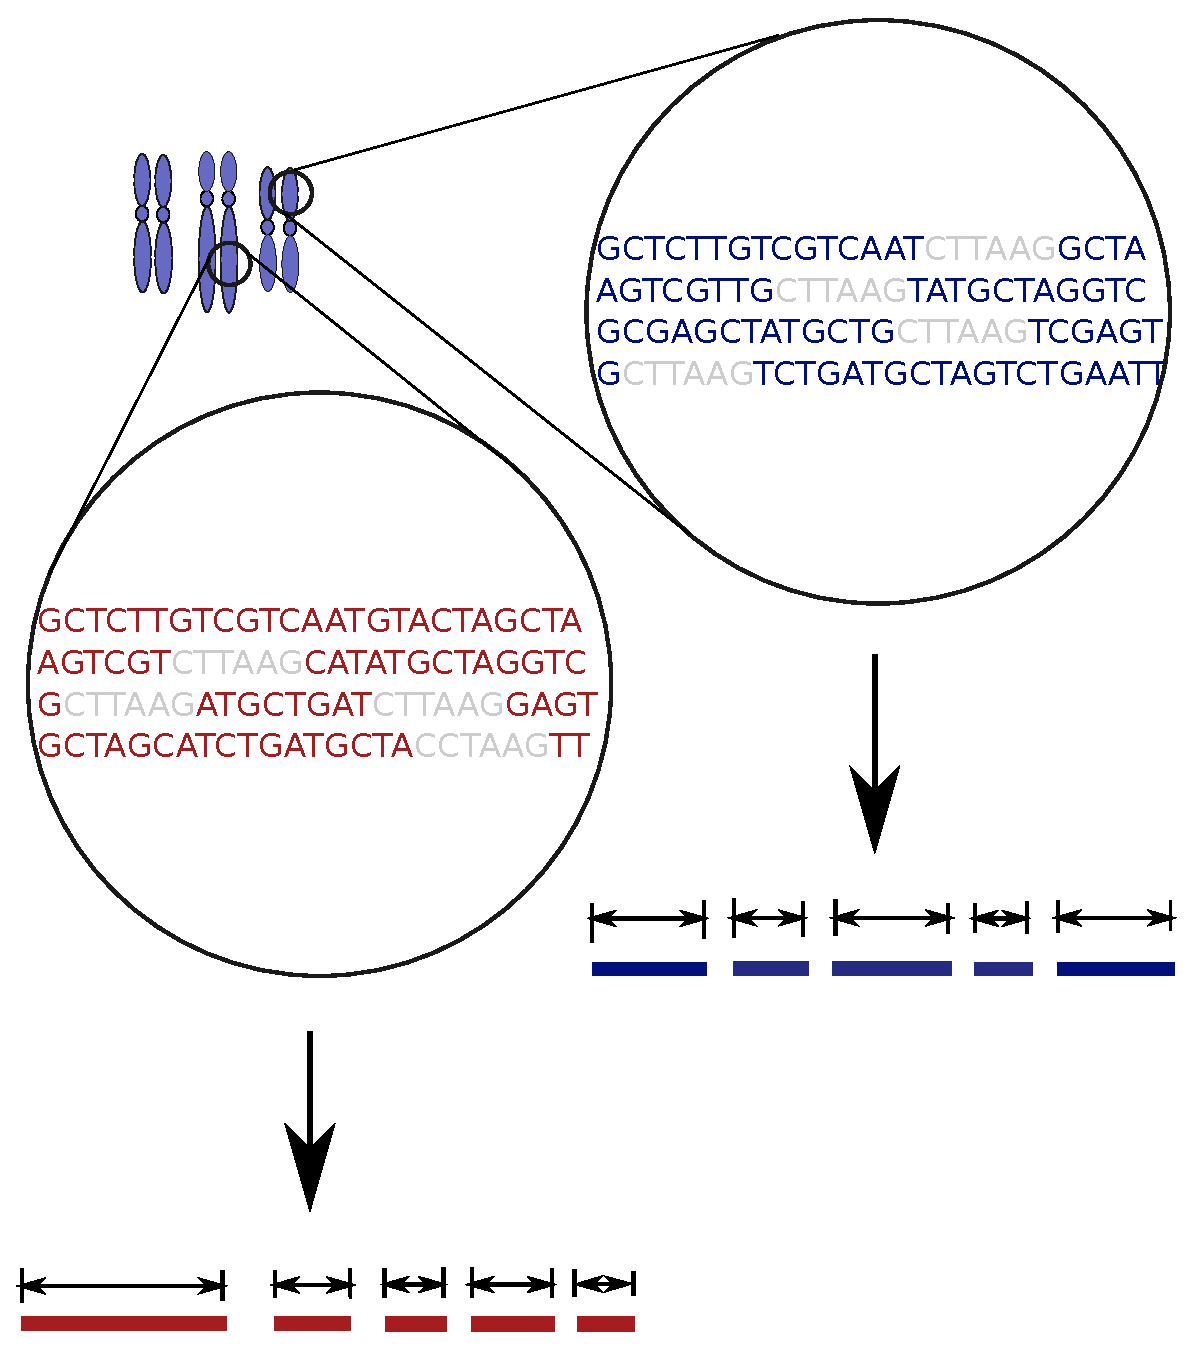
\includegraphics[width=0.35\textwidth]{./research_exam/slides/ormpub.eps}
\caption{An illustration of the data produced by optical mapping. Optical mapping locates and measures the distance between restriction sites.  Analogous to sequence data, optical mapping data is produced for multiple copies of the same genome, and overlapping single molecular maps are analyzed to produce a map for each chromosome.  }
\label{figure:fig1}
\end{figure}


Although optical mapping data has been used for structural variation detection \cite{teague}, scaffolding and validating contigs for several large sequencing projects --- including those for various prokaryote species \cite{reslewic,zhou,zhou2}, \emph{Oryza sativa} (rice) \cite{rice2}, maize \cite{Zhou09}, mouse \cite{church}, goat \cite{GOAT}, \emph{Melopsittacus Undulatus} (budgerigar) \cite{gigadb}, and \emph{Amborella trichopoda} \cite{amborella} --- there exist few non-proprietary tools for analyzing this data. Furthermore, the currently available tools are extremely slow because most of them were specifically designed for smaller, prokaryote genomes.



% TODO CHUCK asked "was in 2014? Any follow on work?"
\subparagraph{Our Contribution.}
We present the first index-based method for aligning contigs to an optical map.
We call our tool $\twin$ to illustrate the association between the assembly and optical map as two representations of the genome sequence.  The first step of our procedure is to \emph{in silico} digest the contigs with the set of restriction enzymes, computationally mimicking how each restriction enzyme would cleave the short segment of DNA defined by the contig.  Thus, \emph{in silico digested contigs} are miniature optical maps that can be aligned to the much longer (sometimes genome-wide) optical maps.  The objective is to search and align the \emph{in silico} digested contigs to the correct location in the optical map.
By using a suitably-constructed FM-Index data structure~\cite{fm2005} built on the optical map,  we show that alignments between contigs and optical maps can be computed in time that is faster
than competing methods by more than two orders of magnitude.


$\twin$ takes as input a set of contigs and an optical map, and produces a set of alignments.  The alignments are output in Pattern Space Layout (PSL) format, allowing them to be visualized using any PSL visualization software, such as IGV~\cite{igv}.  $\twin$ is specifically designed to work on a wide range of genomes, anything from relatively small genomes, to large eukaryote genomes.  Thus, we demonstrate the effectiveness of $\twin$ on \emph{Yersinia kristensenii}, rice, and budgerigar genomes.  Rice and budgerigar have genomes of total sizes 430 Mb and 1.2 Gb, respectively. \emph{Yersinia kristensenii}, a bacteria with genome size of 4.6 Mb, is the smallest genome we considered.   Short read sequence data was assembled for these genomes, and the resulting contigs were aligned to the respective optical map.   We compared the performance of our tool with available competing methods; specifically, the method of Valouev et al.~\cite{Valouev06} and SOMA~\cite{Nagarajan08}.  $\twin$ has superior performance on all datasets, and is demonstrated to be the only current method that is capable of completing the alignment for the budgerigar genome in a reasonable amount of CPU time; SOMA~\cite{Nagarajan08} required over 77 days of machine time to solve this problem, whereas, $\twin$ required just 35 minutes. Lastly, we verify our approach on simulated \emph{E. coli} data by showing our alignment method found correct placements for the \emph{in silico} digested contigs on a simulated optical map.     $\twin$ is available for download at \url{http://www.cs.colostate.edu/twin}.

\subparagraph{Roadmap.}
We review related tools for the problem in the remainder of this section. Section~\ref{sec-background-twin}
then sets notation and formally lays the data structural tools we make use of.
Section~\ref{sec-methods-twin} gives details of our approach. We report our experimental results in
Section~\ref{sec-results-twin}. Finally, Section~\ref{sec-discussion} offers reflections and some potentially
fruitful avenues future work may take.

\subparagraph{Related Work.}
The most recent tools to make use of optical mapping data in the context of assembly are AGORA~\cite{agora} and SOMA~\cite{Nagarajan08}. AGORA~\cite{agora} uses the optical map information to constrain de Bruijn graph construction with the aim of improving the resulting assembly. SOMA~\cite{Nagarajan08} is a scaffolding method that uses an optical map and is specifically designed for short-read assemblies. SOMA requires an alignment method for scaffolding and implements an $\bigO(n^2 m^2)$-time dynamic programming algorithm. Gentig~\cite{Anantharaman01}, and software developed by Valouev et al.~\cite{Valouev06} also use dynamic programming to address the closely related task of finding alignments between optical maps. Gentig is not available for download.  BACop~\cite{Zhou09} also uses a dynamic programming algorithm and corresponding scoring scheme that gives more weight to contigs with higher fragment density. Antoniotti et al.~\cite{antoniotti} consider the unique problem of validating an optical map by using assembled contigs. This method assumes the contigs are error-free. Optical mapping data was produced for Assemblathon 2~\cite{bradnam2013assemblathon}.















\subsection{Background}
\label{sec-background-twin}


\subparagraph{Optical Mapping.}
From a computational point of view, restriction mapping (by optical or other means) is a process that takes two
strings: a genome $\A[1,n]$ and a restriction sequence $\B[1,b]$, and produces
an array (string) of integers $\M[1,m]$, such that $\M[i] = j$ if and only if
$\A[j..j+b] = \B$ is the $i$th occurrence of $\B$ in $\A$.

For example, if we let $\B = \mbox{\emph{act}}$ and
\begin{center}
\resizebox{\textwidth}{!}{\begin{tabular}{p{0.4cm}*{22}{p{0.4cm}}}
& $\scriptstyle 1 $& $\scriptstyle 2 $& $\scriptstyle 3$& $\scriptstyle 4 $& $\scriptstyle 5 $&
$\scriptstyle 6 $& $\scriptstyle 7 $& $\scriptstyle 8 $& $\scriptstyle 9 $& $\scriptstyle 10$&
$\scriptstyle 11 $& $\scriptstyle 12 $& $\scriptstyle 13$& $\scriptstyle 14 $& $\scriptstyle 15 $&
$\scriptstyle 16 $& $\scriptstyle 17 $& $\scriptstyle 18 $& $\scriptstyle 19 $& $\scriptstyle 20$&
$\scriptstyle 21 $& $\scriptstyle 22 $\\
$\A = $& $a$ & $t$ & $a$ & $c$ & $t$ & $t$ & $a$ & $c$ & $t$ & $g$ & $g$
&      $a$ & $c$ & $t$ & $a$ & $c$ & $t$ & $a$ & $a$ & $a$ & $c$ & $t$ \\
\end{tabular}}
\end{center}

then we would have
$$\M = 3,7,12,15,20.$$

It will also be convenient to view $\M$ slightly differently, as an array of fragment
sizes, or distances between occurrences of $\B$ in $\A$ (equivalently differences
between adjacent values in $\M$). We denote this \emph{fragment size domain} of $\M$,
as the array $\R[1,m]$, defined such that $\R[i] = (\M[i]-\M[i-1])$, with $\R[1] = \M[1]-1$.
In words, $\R$ contains the distance between occurrences of $\B$ in $\A$.
Continuing with the example above, we have

$$\R = 2,4,5,3,5.$$

Or if we let $\B$ be {\tt act} and  $\A$  = {\tt atacttactggactactaaact} then we would have $\M = 3,7,12,15,20$ and $\R = 2,4,5,3,5$.






\subsection{Methods}
\label{sec-methods-twin}



We find alignments in four steps.  First, we convert contigs from the sequence domain to the optical map domain through the process of \emph{in silico} digestion. Second, an FM-index is built from the sequence of optical map fragment sizes. Third, we execute a modified version of the FM-index backward search algorithm discussed in Subsection~\ref{backward-search} that allows inexact matches.
As a result of allowing inexact matches, there may be multiple fragments in an optical map that could each be a reasonable match for an \emph{in silico} digested fragment, and in order to include all of these as candidate matches, backtracking becomes necessary in the backward search.
For every backward search path that maintains a non-empty interval for the entire query contig, we emit the alignments denoted by the final interval.

\subsubsection{Converting Contigs to the Optical Map Domain}

In order to find alignments for contigs relative to the optical map, we must first convert the strings of bases into the domain of optical maps, that is, strings of fragment sizes.
We do this by performing an \emph{in silico} digest of each contig, which is performing a linear search over its bases, searching for occurrences of the enzyme recognition sequence and then computing the distances between adjacent restriction sites.
These distances are taken to be equivalent to the fragment sizes that would result if the contig's genomic region underwent digestion in a lab.
Additionally, the end fragments of the \emph{in silico} digested contig are removed, as the outside ends are most likely not a result of the optical map restriction enzyme digestion, but rather an artifact of the sequencing and assembly process.


\subsubsection{Building an FM-index from Optical Mapping Data}
\label{subsec-buildfm}



We construct the FM-index for $\ell$, the string of
fragment sizes.
The particular FM-index implementation we use is the SDSL-Lite\footnote{\url{https://github.com/simongog/sdsl-lite}.} \cite{SDSL}
library's \emph{compressed suffix array with integer wavelet tree} data structure\footnote{The exact revision we used was commit ae42592099707bc59cd1e74997e635324b210115.}.


In preparation for finding alignments, we also keep two auxiliary data structures. The first is the suffix array, $\SA_F$, corresponding to our FM-index, which we use to report the positions in $\ell$ where alignments of a contig occur. While we could decode the relevant entries of $\SA$ on demand with the FM-index in $\bigO(p)$ time, where $p$ is the so-called sample period of the FM-index, storing $\SA$ explicitly significantly improves runtime at the cost of a modest increase in memory usage. The second data structure we store is $\M$, which allows us to map from positions in $\ell$ to positions in the original genome in constant time.

\subsubsection{Alignment of Contigs Using the FM-index}
After constructing the FM-index of the optical map, we find alignments between the optical map and the \emph{in silico} digested contigs.


Specifically, we try to find substrings of the optical map fragment sequence $\ell$ that are similar to the string of each \emph{in silico} digested contig's non-end fragments $F$ satisfying an alignment goodness metric suggested by Nagarajan et al. \cite{Nagarajan08} \footnote{N.B. Alternative goodness metrics could be substituted.  They must satisfy the property that pairs of strings considered to align well are composed of substrings that are also considered to align well would also work.}:
\begin{displaymath}
\Bigl \lvert \sum_{i=s}^{t}F_i - \sum_{j=u}^{v}\ell_j \Bigr \rvert \le F_\sigma \sqrt{\sum_{j=u}^{v}\sigma_{j}^{2}},
\end{displaymath}
where a parameter $F_\sigma$  will affect the precision/recall tradeoff.


This computation is carried out using a modified FM-index backward search.
A simplified, recursive version of our algorithm for finding alignments is shown in Figure~\ref{match}.
The original FM-index backward search proceeds by finding a succession of intervals in the suffix array of the original text that progressively match longer and longer suffixes of the query string, starting from the rightmost symbol of the query.   Each additional symbol in the query string is matched in a process taking two arguments: 1) a suffix array interval, the $\Y$-interval, corresponding to the suffixes in the text, $\ell$, whose prefix matches a suffix of the query string, and 2) an extension symbol $c$.  The process returns a new interval, the $c\Y$-interval, where a prefix of each text suffix corresponding to the new interval is a left extension of the previous query suffix. This process is preserved in $\twin$, and is represented by the function \emph{BackwardSearchOneSymbol} in the $\twin$ algorithm, displayed in Figure~\ref{match}.


Since the optical map fragments include error from the measurement process,
it cannot be assumed an \emph{in silico} fragment size will exactly match the optical map fragment size from the same locus in the genome.
To accommodate these differences, we determine a set of distinct candidate match fragment sizes, $D$, each similar in size to the next fragment to be matched in our query. These candidates are drawn from the
interval of the BWT currently active in our backward search.
We do this by a wavelet tree traversal function provided by SDSL-Lite, which implements the algorithm described in~\cite{GNPtcs11} and takes $\bigO(|D|\log(f/\Delta))$ time. This is represented by the function \emph{RestrictedUniqueRangeValues} in Figure~\ref{match}. We emphasise that, due to the large alphabet of $\ell $, the wavelet tree's ability to list unique values in a range efficiently is vital to overall performance. Unlike in other applications where the FM-index is used for approximate pattern matching (e.g. read alignment), we cannot afford a bruteforce enumeration of the alphabet at each step in the backward search.

These candidates are chosen to be within a reasonable noise tolerance, $t$, based on assumptions about the distribution of optical measurement error around the true fragment length.
Since there may be multiple match candidates in the BWT interval of the optical map for a query fragment, we extend the backward search with backtracking so each candidate size computed from the wavelet tree is evaluated.  That is, for a given \emph{in silico} fragment size (i.e. symbol) $c$, every possible candidate fragment size, $c'$, that can be found in the optical map in the range $c - t \ldots c + t$ and in the interval $s \ldots e$ (of the BWT) for some tolerance $t$ is used as a substitute in the backward search. Each of these candidates is then checked to ensure that a left extension would still satify the goodness metric, and then used as the extension symbol in the backward search.  So it is actually a set of $c'\Y$-intervals that is computed as the left extension in $\twin$.  Additionally, small DNA fragments may not adhere sufficiently to the glass surface and can be lost in the optical mapping process, so we also branch the backtracking search both with and without small \emph{in silico} fragments to accommodate the uncertainty.

Each time the backward search algorithm successfully progresses throughout the entire query (i.e. it finds some approximate match in the optical map for each fragment in the contig query), we take the contents of the resulting interval in the $\SA$ as representing a set of likely alignments.










\renewcommand{\algorithmiccomment}[1]{\hskip0em$\triangleright$ #1}
\begin{figure}
%%\begin{algorithm}[t]
\begin{algorithmic}

\Procedure{Match}{$s$,$e$,$q$,$h$}
\If{$h = -1$}
\State \Comment{Recursion base case.  Suffix array indexes $s .. e$ denote original query matches.}
\State{ \emph{Emit}$(s, e)$}
\Else
\State \Comment{The next symbol to match, $c$, is the last symbol in the query string.}
\State $c \leftarrow q[h]$
\State \Comment{Find the approximately matching values in $\BWT[s \ldots e]$, within tolerance $t$.}
\State $D \leftarrow$ \emph{RestrictedUniqueRangeValues}(s, e, $c + t$, $c - t$)
\State \Comment{Let $c'$ be one possible substitute for $c$ drawn from $D$}
\ForAll{$c' \in D$}
\State \Comment{If Equation 1 is still satisified with $c' $ and $c$, ...}
\If{ $\Bigl \lvert \sum_{i=0}^{|q|-h}\SA[s]_i + c' - \sum_{j=h}^{|q|-1}q_j - c \Bigr \rvert \le F_\sigma \sqrt{\sum_{j=0}^{|q|-h}\sigma_{j}^{2}}$
}
\State \Comment{... determine the suffix array range of the left extension of $c'$.}
\State $s', e' \leftarrow$ \emph{BackwardSearchOneSymbol}($s,e,c'$)
\State \Comment{Recurse to attempt to match the currently unmatched prefix.}
\State \textsc{Match}($s', e', q, h - 1$)
\EndIf
\EndFor
\EndIf
\EndProcedure
\end{algorithmic}


%\end{algorithm}
\caption{\textsc{Match}($s$, $e$, $q$, $h$) Provided a suffix array start index $s$ and end index $e$, query string $q$, and rightmost unmatched query string index $h$ (initially $s=1$, $e=m$, $h=|q| - 1$), emit alignments of an \emph{in silico} digested contig to an optical map.}
\label{match}

\end{figure}


\subsubsection{Output of Alignments in PSL format}
For each \emph{in silico} digested contig that has an approximate match in the optical map, we emit the alignment, converting positions in the fragment string $\ell$ to positions in the genome using the $\M$ table. We provide a script to convert the human readable output into PSL format.
\subsection{Results}
\label{sec-results-twin}

We evaluated the performance of $\twin$ against the best competing methods on \emph{Yersinia kristensenii}, rice and budgerigar.  These three genomes were chosen because they have available sequence and optical mapping data and are diverse in size.   For each dataset, we compared the runtime, peak memory usage, and the number of contigs for which at least one alignment was found for $\twin$, SOMA~\cite{Nagarajan08}, and the software of Valouev et al.~\cite{Valouev06}.  Peak memory was measured as the maximum resident set size as reported by the operating system.  Runtime is the user process time, also reported by the operating system.   SOMA~\cite{Nagarajan08} v2.0 was run with example parameters provided with the tool and the software of Valouev et al.~\cite{Valouev06} was run with its scoring parameters object constructed with arguments (0.2, 2, 1, 5, 17.43, 0.579, 0.005, 0.999, 3, 1). $\twin $ was run with $D_\sigma = 4$, $t = 1000$, and $[250 \ldots 1000]$ for the range of small fragments.
Gentig~\cite{Anantharaman01} and BACop~\cite{Zhou09} were not available for download so we did not test the data using these approaches.

The sequence data was assembled for  \emph{Yersinia kristensenii}, rice and budgerigar by using various assemblers.
The relevant assembly statistics are given in Table~\ref{tab:assembly_stats}.  An important statistic in this table is the number of contigs that have at least two restriction sites, since contigs with fewer than two are unable to be aligned meaningfully by any method, including $\twin$.  This statistic was computed to reveal cases of ambiguity in placement from lack of information. Indeed, Assemblathon~2 required there to be nine restriction sites present in a contig to align it to the optical mapping data \cite{bradnam2013assemblathon}.  All experiments were performed on Intel x86-64 workstations with sufficient RAM to avoid paging, running  64-bit Linux.

\begin{table}[h]
  \centering
  \caption{Assembly and genome statistics for \emph{Yersinia kristensenii}, rice and budgerigar.  The assembly statistics were obtained from Quast. \cite{quast}.}
\resizebox{\textwidth}{!}{\begin{tabular}{| p{0.20\linewidth} |
p{0.15\linewidth} |
p{0.15\linewidth} |
p{0.45\linewidth} |}
\hline
Genome                     		 			 	& N50   	& Genome Size 		& No. of Contigs with  $\geq$ 2 restriction sites\\

\hline
\emph{Y. kristensenii}     	 		         & 30,719 	& 4.6 Mb 				& 92 \\
Rice                       		 		         	& 5,299  	& 430 Mb 				& 3,103 \\
Budgerigar                     	         			         	& 77,556 	& 1.2 Gb 				& 10,019 \\
\hline
\end{tabular}}

\label{tab:assembly_stats}
\end{table}


The experiments for \emph{Yersinia kristensenii}, rice and budgerigar illustrate how each of the programs' running time scale as the size of the genome increases.  However, due to the possibility of mis-assemblies in these draft genomes, comparing the actual alignments could possibly lead to erroneous conclusions.  Therefore, we will verify the alignments using simulated \emph{E. coli} data.  See Subsection \ref{sec:ecoli-twin} for this experiment.



\subsubsection{Performance on \emph{Yersinia kristensenii}}
\label{sec:pro_genome}

The sequence and optical map data for  \emph{Yersinia kristensenii} are described by Nagarajan \emph{et al.} \cite{Nagarajan08}.  The \emph{Yersinia kristensenii} ATCC 33638 reads were generated using 454 GS 20 sequencing and assembled using SPAdes version 3.0.0 \cite{spades} using default parameters.   Contigs from this assembly were aligned against an optical map of the bacterial strain generated by OpGen using the AfIII restriction enzyme.  There are approximately 1.4 million single-end reads for this dataset, and they were obtained from the NCBI Short Read Archive (accession SRX013205).  Of the 92 contigs that could be aligned to the optical map, the software of  Valouev et al. aligned 91 contigs, SOMA aligned 54 contigs, and $\twin$ aligned 61 contigs.  Thus, $\twin$ found more alignments than SOMA, and did so faster. It should be noted that, for this dataset, all three tools had reasonable runtimes. However, while the software of Valouev et al. found more alignments, our validation experiments (below) suggest these results may favor recall over precision, and many of the additional alignments may not be credibled.


\subsubsection{Performance on Rice Genome}
\label{section:rice}

The second dataset consists of approximately 134 million 76 bp paired-end reads from \emph{Oryza sativa Japonica} rice, generated by Illumina, Inc. on the Genome Analayzer (GA) IIx platform, as described by Kawahara \emph{et al.} \cite{kawahara2013improvement}.   These reads were obtained from the NCBI Short Read Archive (accession SRX032913) and assembled using SPAdes version 3.0.0 \cite{spades} using default parameters.  The optical map for rice was constructed by Zhou \emph{et al.} \cite{rice2} using SwaI as the restriction enzyme.  This optical map was assembled from single molecule restriction maps into 14 optical map contigs, labeled as 12 chromosomes, with chromosome labels 6 and 11 both containing two optical map contigs.

Again, $\twin$ found alignments for more contigs than SOMA on the rice genome.  SOMA and $\twin$ found alignments for 2,434, and 3,098 contigs, respectively, out of 3,103 contigs that could be aligned to the optical map.  However, while SOMA required over 29 minutes to run, $\twin$ required less than one minute.
The software of Valouev executed faster than SOMA (taking around 3 minutes), though still several times slower than $\twin$ on this modest sized genome.


\subsubsection{Performance on Budgerigar Genome}
\label{section:parrot}

The sequence and optical map data for the budgerigar genome were generated for the Assemblathon~2 project of Bradnam \emph{et al.} \cite{bradnam2013assemblathon}.   Sequence data consists of  a combination of Roche 454, Illumina, and Pacific Biosciences reads, providing 16x, 285x, and 10x coverage (respectively) of the genome.  All sequence reads are available at the NCBI Short Read Archive (accession  ERP002324).  For our analysis we consider the assembly generated using Celera~\cite{celera}, which was completed by the CBCB team (Koren and Phillippy) as part of  Assemblathon 2~\cite{bradnam2013assemblathon}.  The optical mapping data was created by Zhou, Goldstein, Place, Schwartz, and Bechner using the SwaI restriction enzyme and consists of 92 separate pieces.
As with the two previous data sets, $\twin$ found alignments for more contigs than SOMA on the budgerigar genome.  SOMA and $\twin$ found alignments for 9,668, and 9,826 contigs, respectively, out of 10,019 contigs that could be aligned to the optical map.  However,  SOMA required over 77 days of CPU time and $\twin$ required 35 minutes.  The software of Valouev et al. returned 9,814 alignments and required over an order of magnitude (6.5 hours) of CPU time.  Hence, $\twin$ was the only method that efficiently aligned the \emph{in silico} digested budgerigar genome contigs to the optical map.  It should be kept in mind that the competing methods were developed for prokaryote genomes and so we are repurposing them at a scale for which they were not designed.   Lastly, the amount of memory used by all the methods on all experiments was low enough for them to run on a standard workstation.

We were forced to parallelize SOMA due to the enormous amount of CPU time SOMA required for this dataset.  To accomplish this task, the FASTA file containing the contigs was split into 300 different files, and then IPython Parallel library was used to invoke up to two instances of SOMA on each machine from a set of 150 machines.  Thus, when using a cluster with up to 300 jobs concurrently, the alignment for the budgerigar genome took about a day of wall clock time. In contrast, we ran the software of Valouev et al. and $\twin$ with a single thread running on a single core.  However, it should be noted that the same parallelization could have been accomplished for both these software methods too. Also, even with parallelization of SOMA, $\twin$ is still an order of magnitude faster than it.



\begin{table}[h]
\centering
\caption{{\bf Comparsion of the alignment results for $\twin$ and competing method.}  The performance of $\twin$ was compared against SOMA \cite{Nagarajan08} and the method of Valouev et al.~\cite{Valouev06} using the assembly and optical mapping data for \emph{Yersinia Kristensenii}, rice, and budgerigar.  Various assemblers were used to assemble the data for these species.  The relevant statistics and information concerning these assemblies and genomes can be found in Table \ref{tab:assembly_stats}.  The peak memory is given in megabytes (mb).  The running time is reported in seconds (s), minutes (m), hours (h), and days. }

\resizebox{\textwidth}{!}{\begin{tabular}{|
p {0.22\linewidth} |
p {0.20\linewidth} |
p {0.15\linewidth} |
p {0.13\linewidth} |
p {0.25\linewidth} | }

\hline
{\bf Genome} 			&  {\bf Program}	& {\bf Memory }	& {\bf Time } 			& {\bf Aligned Contigs} \\

\hline
\hline
\emph{Y. Kristensenii} & & &  & \\
\hline

& Valouev \emph{et al.} 	& 1.81 		& .17 s 			& 91  \\
& SOMA 				& 1.71 		& 7.32 s 			& 54 \\
& $\twin$
& 18  		& .06 s
& 65\\
\hline
\hline
Rice & & &   & \\
\hline

& Valouev \emph{et al.} 	& 11.25 		& 2 m 57 s 			& 2,676  \\
& SOMA 				& 7.94 		& 29 m 38 s 		& 2,434 \\
& $\twin$
& 18.25  		&  50 s 			&  3,098\\
\hline
\hline
Budgerigar & & & & \\
\hline

& Valouev \emph{et al.} 	& 390  			& 6.5 h 		& 9,814 \\
& SOMA 				& 380.95  		& 77.2 d 		& 9,668 \\
& $\twin$                         &127.112                  &  35 m           & 9,826\\

\hline
\end{tabular}}
\label{tab:possible_columns}
\end{table}



\subsubsection{Alignment Verification}
\label{sec:ecoli-twin}

We compared the alignments given by $\twin$ against the alignments of the contigs of an \emph{E. coli} assembly to the \emph{E. Coli} (str. K-12 substr. MG1655) reference genome.  Our prior experiments involved species for which the reference genome may have regions that are mis-asssembled and therefore, contig alignments to the reference genome may be inaccurate and cannot be used for comparison and verification of the \emph{in silico} digested contig alignment.   The \emph{E. coli} reference genome is likely to contain the fewest errors and thus, is the one we used for assembly verification.  The sequence data consists of approximately 27 million paired-end 100 bp reads from \emph{E. coli} (str. K-12 substr. MG1655) generated by Illumina, Inc. on the Genome Analayzer (GA) IIx platform, and  was obtained from the NCBI Short Read Archive (accession ERA000206), and was assembled using SPAdes version 3.0.0 \cite{spades} using default parameters.  This assembly consists of 160 contigs; 50 of which contain two restriction sites, the minimum required for any possible optical alignment, and complete alignments with minimal (\textless 800 bp) total in/dels relative to the reference genome.

We simulated an optical map using the reference genome for \emph{E. coli} (str. K-12 substr. MG1655) since there is no publicly available one for this genome.

The 50 contigs that contained more than two restriction sites were aligned to the reference genome using BLAT~\cite{blat}.  These same contigs were then \emph{in silico} digested and aligned to the optical map using $\twin$.  The resulting PSL files were then compared.  $\twin$ found alignment positions within 10\% of those found by BLAT for all 50 contigs, justifying that our method is finding correct alignments.  We repeated this verification approach with both SOMA and the software from Valouev.  All of SOMA's reported alignments had matching BLAT alignments, while of the 49 alignments the software from Valuoev reported, only 18 could be matched with alignments from BLAT.

\subsection{Discussion and Conclusions}
\label{sec-discussion}

We demonstrated that $\twin$, an index-based algorithm for aligning \emph{in silico} digested contigs to an optical map, gave over an order of magnitude improvement to runtime without sacrificing alignment quality. Our results show that we are able to handle genomes at least as large as the budgerigar genome directly, whereas SOMA cannot feasibly complete the alignment for this genome in a reasonable amount of time without significant parallelization, and even then is orders of magnitude slower than $\twin$. Indeed, given its performance on the budgerigar genome, and its $\bigO(m^2 n^2)$ time complexity, larger genomes seem beyond SOMA.  For example, the loblolly pine tree genome, which is approximately 20 Gb \cite{pinetree}, would take SOMA approximately 84 machine years, which, even with parallelization, is prohibitively long.

Optical mapping is a relatively new technology, and thus, with so few algorithms available for working with this data, we feel there remains good opportunities for developing more efficient and flexible methods. Dynamic programming optical map alignment approaches are still important today, as the assembly of the consensus optical maps from the individually imaged molecules often has to deal with missing or spurious restriction sites in the single molecule maps when enzymes fail to digest a recognition sequence or the molecule breaks.  Though coverage is high (e.g. about 1,241 Gb of optical data was collected for the 2.66 Gb goat genome), there may be cases where missing restriction site errors are not resolved by the assembly process.   In these rare cases (only 1\% of alignments reported by SOMA on parrot contain such errors) they will inhibit $\twin$'s ability to find correct alignments.  In essence, $\twin$ is trading a small degree of sensitivity for a huge speed increase, just as other index based aligners have done for sequence data.  Sir\'{e}n et al.~\cite{dag_method} recently extended the Burrows-Wheeler transform (BWT) from strings to acyclic directed labeled graphs and to support path queries. In Section \ref{sec:kohdista} we'll examine an adaptation of this method for optical map alignment that allows for the efficient handling of missing or spurious restriction sites.

In later work~\cite{muggli2015misassembly} we showed an ensemble of optical map alignments produced by $\twin$ and alignments of reads to contigs could produce superior statistical performance on misassembly detection.


\section[Kohdista: A Succinct Solution to Raw Optical Map Alignment]{Kohdista: A Succinct Solution to Raw Optical Map Alignment\protect\footnote{Martin D. Muggli, Simon J. Puglisi, and Christina Boucher. A Succinct Solution to Rmap
		Alignment. In Laxmi Parida and Esko Ukkonen, editors, {\it 18th International Workshop on Al-
		gorithms in Bioinformatics (WABI 2018)}, volume 113 of {\it Leibniz International Proceedings
		in Informatics (LIPIcs)}, pages 12:1–12:16, Dagstuhl, Germany, 2018. Schloss Dagstuhl–
		Leibniz-Zentrum fuer Informatik.}}
\label{sec:kohdista}

In this section, we build on the work from TWIN to solve a noisier form of optical mapping data.  In practice, the method developed here could aid approaches like misSEQuel because \mbox{misSEQuel} takes a whole genome optical map as input, but these themselves must be assembled by an overlap-layout-consensus process from the data described in this section.


\subsection{Introduction}




Genome-wide optical maps are ordered high-resolution restriction maps that give the position of occurrence of  restriction cut sites corresponding to one or more restriction enzymes.  These genome-wide optical maps are assembled using an overlap-layout-consensus approach using  raw optical map data, which are referred to as {\em Rmaps}.  Hence, Rmaps are akin to reads in genome sequencing.  To date, however, there is no efficient, non-proprietary method for finding pairwise alignments between Rmaps, which is the first step in assembling genome-wide maps.

Several existing methods are superficially applicable to Rmap pairwise alignments but all programs either struggle to scale to even moderate size genomes or require significant further adaptation to the problem. Several methods exhaustively evaluate all pairs of Rmaps using dynamic programming.  One of these is the method of Valouev {\it et al.}~\cite{Valouev06}, which is capable of solving the problem exactly but requires over 100,000 CPU hours to compute the alignments for rice~\cite{valouev2006algorithm}.  The others are SOMA~\cite{Nagarajan08} and MalignerDP~\cite{maligner} which are designed only for semi-global alignments instead of overlap alignments, which are required for assembly.

Other methods reduce the number of map pairs to be individually considered by initially finding seed matches and then extending them through more intensive work.  These include OMBlast~\cite{omblast}, OPTIMA~\cite{optima}, and MalignerIX~\cite{maligner}.  These, along with MalignerDP, were designed for a related alignment problem of aligning consensus data but cannot consistently find high quality Rmap pairwise alignments in reasonable time as we show later.  This is unsurprising since these methods were designed for either already assembled optical maps or \emph{in silico} digested sequence data for one of their inputs, both having a lower error rate than Rmap data.

{\bf Our contributions.}  In this paper, we present a fast, error-tolerant method for performing pairwise Rmap alignment that makes use of a novel FM-index based data structure.  Although the FM-index can naturally be applied to short read alignment~\cite{bwa,bowtie}, it is nontrivial to apply it to Rmap alignment.  The difficulty arises from: (1) the abundance of missing or false cut sites, (2) the fragment sizes require inexact fragment-fragment matches (e.g. 1,547 bp and 1,503 bp represent the same fragment), (3) the Rmap sequence alphabet consists of all unique fragment sizes and is so extremely large (e.g., over 16,000 symbols for the goat genome).  The second two challenges render inefficient the standard FM-index backward search algorithm, which excels at exact matching over small alphabets. The first (and most-notable) challenge requires a more complex index-based data structure be used to create an aligner that is robust for insertion and deletion of cut sites. To overcome the mismatch cut site challenge while still accommodating the other two, we develop $\dopp$, an index-based Rmap alignment program that is capable of finding all pairwise alignments in large eukaryote organisms.

We first abstract the problem to that of approximate-path matching in a directed
acyclic graph (DAG). The $\dopp$ method then indexes a set of Rmaps represented
as a DAG, using a modified form of the {\em generalized compressed suffix array (GCSA)}, which is
a derivative of the FM-index developed by Sir\'{e}n {\it et al.}~\cite{dag_method}.  The principle insight of our work is that while GCSA is able to efficiently match all similar paths concurrently, it was designed for indexing variations observed in a collection of sequences.
In contrast, our work indexes variations that are instead speculative, based on the Rmap error profile.  Lastly, we demonstrate that challenges posed by the inexact fragment sizes and alphabet size can be overcome, specifically in the context of the GCSA, via careful use of a wavelet tree~\cite{GNPtcs11,wabi2014}.

We verify our approach on simulated {\em E. coli} Rmap data by showing that $\dopp$ achieves similar sensitivity and specificity to Valouev {\it et al.}, and with more permissive alignment acceptance criteria 90\% of Rmap pairs simulated from overlapping genomic regions.
We also show the utility of our approach on larger eukaryote genomes by demonstrating that existing published methods require more than 151 hours of CPU time to find all pairwise alignments in the plum Rmap data; whereas, $\dopp$ requires 31 hours. Thus, we present the first fully-indexed method capable of finding all match patterns in the pairwise Rmap alignment problem.



\subsection{Background}
\label{sec-background-koh}







\noindent{\bf More Details of Optical Mapping.}



A detail omitted in $\twin$ is that the whole genome restriction map $\R$ is actually a consensus sequence formed from millions of erroneous Rmap sequences.
The optical mapping system produces millions of Rmaps for a single genome. It is performed on many cells of an organism and for each cell there are thousands of Rmaps (each at least 250 Kbp in length in publicly available data).
These Rmaps must then be assembled to produce a genome-wide optical map which can then be used in downstream tools such as $\twin$.
Like the final $\R$ sequence, each Rmap is an array of lengths --- or fragment sizes --- between occurrences of $\B$ in $\A$.


There are three types of errors that an Rmap (and hence with lower magnitude and frequency, also the consensus map) can contain: (1) missing and false cuts, which are caused by an enzyme not cleaving at a specific site, or by random breaks in the DNA molecule, respectively; (2) missing fragments that are caused by {\em desorption}, where small ($ < 1$ Kbp ) fragments are lost and so not detected by the imaging system; and (3) inaccuracy in the fragment size due to varying fluorescent dye adhesion to the DNA and other limitations of the imaging process.  Continuing again with the example above where $\R = 2,4,5,3,5$ is the error-free Rmap: an example of an Rmap with the first type of error could be $\R' = 6,5,3,5$ (the first cut site is missing so the fragment sizes 2, and 4 are summed to become 6 in $\R'$); an example of a Rmap with the second type of error would be $\R'' = 2,4,3,5$ (the third fragment is missing); and lastly, the third type of error could be illustrated by $\R''' = 2,4,7,3,5$ (the size of the third fragment is inaccurately given).


\noindent{\bf Frequency of Errors.} In the optical mapping system, there is a 20\% probability that a cut site is missed and a 0.15\% probability of a false break per Kbp, i.e., error type (1) occurs in a fragment.  Popular restiction enzymes in optical mapping experiments recognize a 6 bp sequence giving an expected cutting density of 1 per 4096 bp.  At this cutting density, false breaks are less common than missing restriction sites (approx. $0.25 * .2 = .05$ for missing sites vs. 0.0015 for false sites per bp).  The inaccuracy of the fragment sizes, i.e, error type (3), follows a normal distribution with mean and variance assumed to be 0 bp and $\ell \sigma^2$ ($\sigma = .58$ kbp), respectively~\cite{Valouev06}.







\subsection{The Pairwise Rmap Alignment Problem}




Given a genome $\A[1,n]$ and a restriction enzyme's recognition sequence $\B[1,b]$, the optical mapping system produces Rmaps, which are arrays of lengths---or fragment sizes---between occurrences of $\B$ in $\A$. The background section provides details on the optical mapping process.  Producing Rmap data is an error prone process. Thus, three types of errors can occur: (1) missing and false cuts that delimit fragments; (2) missing fragments; and (3) inaccuracy in the fragment sizes.  For example, let $\R = 2,4,5,3,5$ be an error-free Rmap, then an example of an Rmap with the first type of error could be $\R' = 6,5,3,5$ (the first cut site is missing so the fragment sizes 2, and 4 are summed to become 6 in $\R'$); an example of a Rmap with the second type of error would be $\R'' = 2,4,3,5$ (the third fragment is missing); and lastly, the third type of error could be illustrated by $\R''' = 2,4,7,3,5$ (the size of the third fragment is inaccurately given)



The pairwise Rmap alignment problem aims to align one Rmap (the \emph{query}) $\R_q$ against the set of all other Rmaps in the dataset (the \emph{target}). We denote the target database as $\R_1 \ldots \R_n$, where each $\R_i$  is a sequence of $m_i$ fragment sizes, i.e, $\R_i = [f_{i1}, .., f_{im_i}]$.  An alignment between two Rmaps is a relation between them comprising groups of zero or more consecutive fragment sizes in one Rmap associated with groups of zero or more consecutive fragments in the other.  For example, given $\R_i =  [4, 5, 10, 9, 3]$ and $\R_j = [10, 9, 11]$ one possible alignment is $\{[4,5], [10]\}, \{ [10], [9]\}, \{[9], [11]\}, \{[3], []\}$.  A group may contain more than one fragment (e.g. $[4,5]$) when the restriction site delimiting the fragments is absent in the corresponding group of the other Rmap (e.g $[10]$). This can occur if there is a false restriction site in one Rmap, or there is a missing restriction site in the other.  Since we cannot tell from only two Rmaps which of these scenarios occurred, for the purpose of our remaining discussion it will be sufficient to consider only the scenario of missed (undigested) restriction sites.



\subsection{Methods}
\label{sec-methods-koh}

We now describe the algorithm behind $\dopp$.
Three main insights enable our index-based aligner for Rmap data: 1) abstraction of the alignment problem to a finite automaton; 2) use of the GCSA for storing and querying the automaton; and 3) modification of backward search to use a wavelet tree in specific ways to account for the Rmap error profile.

\subsubsection{Finite Automaton}

Continuing with the example in the background section, we want to align $\R' = 6,5,3,5$ to $\R''' = 2,4,7,3,5$ and vice versa.  To accomplish this we cast the Rmap alignment problem to that of matching paths in a finite automaton.  A finite automaton is  a directed, labeled graph that defines a \emph{language}, or a specific set of sequences composed of vertex labels.  A sequence is recognized by an automaton if it contains a matching path: a consecutive sequence of vertex labels equal to the sequence. We represent the target Rmaps as an automaton and the query as a path in this context.

The automaton for our target Rmaps can be constructed as follows.  First concatenate the $\R_1 \ldots \R_n$ together into a single sequence with each Rmap separated by  a special symbol which will not match any query symbol. Let $\R^*$ denote this concatenated sequence. Hence, $\R^* = [f_{11},..,f_{1m_1}, \ldots, f_{n1},..,f_{nm_n}]$.  Then, construct an initial finite automaton $\A = (V, E)$ for $\R^*$ by creating a set of vertices $v^i_1 .. v^i_m$, one vertex labeled with each fragment length and edges connecting them. Also, introduce to $\A$  a {\em starting vertex} $v_1$ labeled with $\#$ and a {\em final vertex} $v_f$ labeled with the character $\$$.  All other vertices in $\A$ are labeled with integral values.  This initial set of vertices and edges is called the {\em backbone}.  The backbone by itself is only sufficient for finding alignments with no missing cut sites in the query.  The backbone of an automaton constructed for a set containing $\R'$ and $\R''$ would be  $\#, 6, 5, 3, 5, 999, 2, 4, 3, 5\$$, using $999$ as an unmatchable value.  Next, extra vertices (``skip vertices'') and extra edges are added to $\A$ to allow for the automaton to accept all valid queries.  Figure \ref{fig:example}(a) illustrates the construction of $\A$ for a single Rmap with fragment sizes $2, 3, 4, 5, 6$.

\subsubsection{Skip Vertices and Skip Edges}
We introduce extra vertices labeled with {\em compound fragments} to allow missing cut sites (first type of error) to be taken into account in querying the target Rmaps.  We refer to these as {\em skip vertices} as they provide alternative path segments which skip past two or more backbone vertices. Thus, we add a {\em skip vertex} to $\A$ for every $o+1$ length run of consecutive vertices in the backbone where $1 < o < order$ and  \emph{order} is the maximum number of consecutive missed cut sites to be accommodated.  First order skip vertices are each labeled with the sum of two consecutive backbone vertices.  Second order skip vertices are each labeled with the sum of three consecutive backbone vertices. The vertex labeled with $7$ connecting $2$ and $5$ in \ref{fig:example}(a) is an example of a skip vertex.  Likewise, $5, 9, 11$ are other skip vertices.

\begin{figure}[h!] %{1.0\textwidth}
%\centering
\includegraphics[width=\textwidth]{gcsa_paper/content/figures/example_combined}
\caption{An example automaton for an Rmap with fragment size sequence $2, 3, 4, 5, 6$.  The memory representation is shown in Table~\ref{bwt-table}. The top half of vertices contains the label, which models a fragment size in Kbp.  The common prefixes of all suffixes spellable from a vertex is written in the bottom half.  Note that there is no ordering of vertices such that all their corresponding suffixes are in lexicographic order;  the leftmost vertex labelled with ``5'' spells suffixes beginning ``5,4,...'' as well as the suffix ``5,9,6,\$'' while the rightmost $5$  spells the suffix ``5,6,\$''. (b) shows the prefix sorted automaton corresponding to the one in (a).  The leftmost vertex $5$ has been duplicated and the outgoing edges of the previous version have been divided between the new replacement instances.  This also divides the suffixes spellable from the prior version.  Now the three $5$ vertices can be ordered based on their common prefixes as [``$5$,$4$,...'',``$5$,$6$,\$'', ``$5$,$9$,$6$, \$'']. }
\label{fig:example}
\end{figure}



\begin{table*}[h!]
  \begin{center}
      \caption{Table listing the three arrays storing the automaton shown in Figure~\ref{fig:example} in memory: $\BWT$, $\M$, and $\F$.}
    
  \begin{tabular}{ccccccccccccc}
  	\hline
		& \$		& 2		& 3		& 4		& 5,4		& 5,6,\$	& 5,9,6,\$	& 6,\$	& 7	& 9,6,\$	& 11,\$	& \# \\
	\hline
$\BWT$	& 6,11	& \#		& 2		& 3,5		& \#		& 4,7		& \#		& 5,9		& 2	& 3,5		& 4,7		& \$ \\
$\M$		& 1		& 10		& 10		& 10		& 1		& 1		& 1		& 1		&10	& 1		& 1 		& 100 \\
$\F$		& 10		& 1		& 1		& 10		& 1		& 10		& 1		& 10		& 1	& 10		& 10		& 1 \\		
	\hline
	\end{tabular}
 \label{bwt-table}
\end{center}
\end{table*}



Finally, we add {\em skip edges} which provide paths around vertices with small labels in the backbone.
These allow a query with a missing fragment to still match.\footnote{Different smallness thresholds for query and target bias toward this scenario, avoiding backtracking in the search.}  Hence, the addition of skip edges allow for desorption (the second type of error) to be taken into account in querying the target Rmaps.



%\begin{figure}[h!t]  \centering
%  \caption{Example automata and corresponding memory representation.}


% \begin{figure}[b]%{.3\textwidth}

% %  \small
% \begin{tabular}{c|p{9mm}p{3mm}p{3mm}}
% & ABWT & M & F  \\
% \hline
% \hline
% \$ & 6 \newline 11 & 1 & 1 \newline 0  \\ \hline
% 2 & \# & 1 \newline 0 & 1  \\ \hline
% 3 & 2 & 1 \newline 0 & 1  \\ \hline
% 4 & 3 \newline 5 & 1 \newline 0 & 1 \newline 0  \\ \hline
% 5,4 & \# & 1 & 1  \\ \hline
% 5,6,\$ & 4 \newline 7 & 1 & 1 \newline 0  \\ \hline
% 5,9,6,\$ & \# & 1 & 1  \\ \hline
% 6,\$ & 5 \newline 9 & 1 & 1 \newline 0  \\ \hline
% 7 & 2 & 1 \newline 0 & 1  \\ \hline
% 9,6,\$ & 3 \newline 5 & 1 & 1 \newline 0  \\ \hline
% 11,\$ & 4 \newline 7 & 1 & 1 \newline 0  \\ \hline
% \# & \$ & 1 \newline 0 \newline 0 & 1   \\
% \end{tabular}
% \caption{Table listing the three arrays storing the automaton shown in Figure~\ref{fig:example} in memory: $\ABWT$, $\M$, and $\F$. Each row in the table delimits elements associated with a particular vertex.}  
%                       \label{bwt-table}
% \end{figure}

%\end{figure}


\subsubsection{Generalized Compressed Suffix Array}


We index the automaton with the GCSA~\cite{dag_method} for efficient storage and path querying.  The GCSA is a generalization of the FM-index for automata and
we will explain the GCSA by drawing on the definition of the (more widely known) FM-index.
%TODO kill previous paragraph?

To generalize the FM-index to automata (from strings), we need to efficiently store the vertices and edges in a manner such that the FM-index properties still hold, allowing the GCSA to support queries efficiently.  An FM-index's compressed suffix array for a string $X$ encodes a relationship between each suffix $Y$ and its left extension.  Hence, this suffix array can be generalized to edges in a graph that represent a relationship between vertices.  The compressed suffix array for a string is a special case where the vertices are labeled with the string's symbols in a non-branching path.

\subsubsection{Prefix-sorted Automata}
Just as backward search for strings is linked to suffix sorting, backward searching in the BWT of the automaton
requires us to be able to sort the vertices (and a special set of the paths) of the automaton in a particular
way. In~\cite{dag_method} this property is called {\em prefix-sortedness}. Let $A = (V,E)$ be a finite automaton,
let $v_{|V|}$ denote its terminal vertex, and let $v \in V$ be a vertex. We say $v$ is {\em prefix-sorted} by
prefix $p(v)$ if the labels of all paths from $v$ to $v_{|V|}$ share a common prefix $p(v)$, and no path from any
other vertex $u \ne v$ to $v_{|V|}$ has $p(v)$ as a prefix of its label. If all
vertices $V$ are prefix-sorted then Automaton $A$ is prefix-sorted. See Figure~\ref{fig:example} for an example of a non-prefix sorted automaton and a
prefix sorted automaton. A non-prefix sorted automaton can be made prefix sorted through a process of duplicating
vertices and their incoming edges but dividing their outgoing edges between the new instances (see~\cite{dag_method}).

Clearly the prefixes $p(v)$ allow us to sort the vertices of a prefix-sorted automaton into lexicographical
order. Moreover, if we consider the list of outgoing edges $(u,v)$, sorted by pairs $(p(u),p(v))$, they are
also sorted by the sequences $\ell(u)p(v)$, where $\ell(u)$ denotes the label of vertex $u$. This (dual sortedness)
property allows backward searching to work over the list of vertex labels (sorted by $p(v)$) in the same way
that is does for the symbols of a string ordered by their following suffixes in normal backward search for
strings.

Each vertex has a set of one or more preceding vertices and therefore, a set of predecessor labels in the
automaton. These predecessor label sets are concatenated to form the automaton analog of the $\BWT$, or $\ABWT$. The sets are concatenated in the
order defined by the above mentioned lexicographic ordering of the vertices. Each element in $\ABWT$ then
denotes an edge in the automaton. An array of bits, $\I$\footnote{$I$ was denoted $F$ in the original GCSA paper.}, marks a `1' for the first element of $\ABWT$
corresponding to a vertex and a `0' for all subsequent elements in that set. Thus, the predecessor labels,
and hence the associated edges, for a vertex with rank $r$ are $\ABWT[\select(r)..\select(r+1)]$. Another
array, $\O$\footnote{$O$ was denoted $M$ in the original GCSA paper}, stores the out degree of each vertex and allows the set of vertex ranks associated with a $\ABWT$
interval to be found using $\rank()$ queries.



\subsubsection{Exact Matching: GCSA Backward Search}


Exact matching with the GCSA is similar to the standard FM-index backward search algorithm. As outlined in the background section, FM-index backward search proceeds by finding a succession of lexicographic ranges that progressively match longer and longer suffixes of the query string, starting from the rightmost symbol of the query. The search maintains two items --- a lexicographic range and an index into the query string --- and the property that the path prefix associated with the lexicographic range is equal to the suffix of the query marked by the query index. Initially, the query index is at the rightmost symbol and the range is $[1..n]$ since every path prefix matches the empty suffix.  The search continues using GCSA's backward search step function, which takes as parameters the next symbol (to the left) in the query (i.e. fragment size in $\R_q$) and the current range, and returns a new range.  The query index is advanced leftward after each backward search step.  In theory, since the current range corresponds to a consecutive range in the $\ABWT$, the backward search could use  $\select()$ queries on a bit vector $\I$ to determine all the edges adjacent to a given vertex and then two FM-index $\LF()$ queries are applied to the limits of the current range to obtain the new one.  GCSA's implementation uses one succinct bit vector per alphabet symbol to encode which symbols precede a given vertex instead of $\I$.  Finally, this new range, which corresponds to a set of edges, is mapped back to a set of vertices using $\rank()$ on the $\M$ bit vector.


\subsubsection{Inexact Matching: GCSA Backward Search Using a Wavelet Tree}



We modified GCSA backward search in the following ways:
(1) we used a wavelet tree to allow efficient retrieval of substitution candidates; (2) we modified the search process to combine consecutive query fragments into compound fragments so as to match fragments in $\R^*$ missing the interposing restriction site; and (3) we introduced backtracking, in order to both try size substitution candidates as well as various combinations of compound fragments. These modifications are further detailed below.

First, in order to accommodate possible errors in fragment size, we determine a set, $\Z$, of candidate fragment sizes that are similar to the next fragment of $\R_q$ to be matched in the query. These candidates are determined by enumerating the distinct symbols in the currently active backward search range of the $\ABWT$\footnote{Recall that this active range, when applied to a lexicographic range, represents the suffixes whose prefixes are the matched portion of the query, while the same range of the $\ABWT$ contains possible extension symbols.} using the wavelet tree algorithm of Gagie {\it et al.}~\cite{GNPtcs11}.  This method was proposed by Muggli {\it et al.}~\cite{wabi2014} for use with an FM-index but was not directly applicable to the originally proposed implementation of GCSA. This is because some of GCSA's theoretical constructs (i.e. $I$) were substituted in implementation for efficiency reasons.  In order to apply the aforementioned  wavelet tree method, we thus resurrect the previously theoretical only bit array $\I$ (which we encode succinctly) as well as symbol array $\ABWT$ (which we encoded with a wavelet tree) into $\dopp$ using the SDSL-Lite library by Gog {\it et al.}~\cite{SDSL}.

To accommodate possible restriction sites that are present in the query Rmap but absent in target Rmaps, we generate compound fragments (i.e. new symbols) by summing pairs and triples of consecutive query fragment size and then querying the wavelet tree for substitutions of these compound fragments. This summing of multiple consecutive fragments is complementary to the skip vertices in the target automaton and accommodates missed restriction sites in the target, just as the skip vertices accommodate missed sites in the query.

Lastly, since there may be multiple match candidates in the $\ABWT$ interval of $\R^*$
for a compound fragment generated from $\R_q$ and multiple compound fragments generated at a given position in $\R_q$, we employ the common practice of adding backtracking to backward search (as is done, for example in the works of Li {\it et al.} and Langmead {\it et al.}).   This is so that each candidate size returned to the search algorithm from the wavelet tree is evaluated; i.e., for a given compound fragment size $f$ generated from $\R_q$, every possible candidate fragment size, $f'$, that can be found in $\R^*$ in the range $f - t \ldots f + t$ and in the interval $s \ldots e$ (of the $\ABWT$ of $\R^*$) for some tolerance $t$ is used as a substitute in the backward search.

\subsection{Results and Discussion}
\label{sec-results-koh}



We evaluated $\dopp$ against the other available optical map alignment software.
Our experiments measured runtime, peak memory, and  alignment quality on simulated {\em E. coli} Rmaps and experimentally generated plum Rmaps.  All experiments were performed on Intel Xeon computers with $\ge$ 16 GB RAM running 64-bit Linux.




\subsubsection{Performance on Simulated E.coli Rmap Data}
\label{sec:ecoli-koh}

To verify the correctness of our method, we simulated a read set from a 4.6 Mbp \emph{E. coli} reference genome as follows:  we started with 1,400 copies of the genome, and then generated 40 random loci within each. These loci form the ends of molecules that would undergo digestion.  Molecules smaller than 250 Kbp were discarded leaving 272 molecules with a combined length equating to 35x coverage depth.  The cleavage sites for the XhoI enzyme were then identified within each of these simulated molecules. We removed 20\% of these at random from each simulated molecule to model partial digestion.  Finally, normally distributed noise was added to each fragment with a standard deviation of .58 kb per 1 kb of the fragment.  Simulated molecule pairs having 16 common conserved digestion sites become the ``ground truth''\footnote{Due to repeats in the restriction map, and apparent repeats at the resolution attainable through optical measurement, some alignments beyond these are expected.} data for testing our method with the others.  Although a molecule would align to itself, these are not included in the ground truth set. This method of simulation was based on the \emph{E. coli} statistics given by Valouev {\it et al.}~\cite{valouev2006algorithm} and resulting in a molecule length distribution as observed in publicly available Rmap data from OpGen, Inc.

Most of the tools were designed for less noisy data but in theory could address all the data error types required. For tools with tunable parameters, we tried aligning the {\it E. coli} Rmaps  with combinations of parameters for each method related to its alignment score thresholds and error model parameters.  We used parameterization giving results similar to those for the default parameters of Valouev {\it et al.}'s method to the extent such parameters did not significantly increasing each tool's runtime.  These same parameterization were used in the next section on plum data.

Even with tuning, we were unable to obtain pairwise alignments on {\it E. coli} for two methods. We found OPTIMA only produced self alignments with its recommended overlap protocol and report its resource use in Table~\ref{tbl-ecoli}.
For MalignerIX, even when we relaxed the parameters to account for the greater sizing error and mismatch cut site frequency, it was also only able to find self alignments.  This is expected as by design it only allows missing sites in one sequence in order to run faster. Thus no further testing was performed with MalignerIX or OPTIMA. We did not test SOMA~\cite{Nagarajan08} as earlier investigation indicate it would not scale to larger genomes~\cite{wabi2014}. We omit TWIN~\cite{wabi2014} as it needs all cut sites to match.

Results on {\it E. coli} are presented in Table~\ref{tbl-ecoli}. $\dopp$ uses $\chi^2$ and binomial CDF thresholds to prune the backtracking search when deciding whether to extend alignments to progressively longer alignments.  More permissive match criteria, using higher thresholds, allows  more Rmaps to be reached in the search and thus to be considered aligned, but it also results in less aggressive pruning in the search, thus lengthening runtime.  As an example, note that when $\dopp$ was configured with a much relaxed CDF threshold of .5 and a binomial CDF threshold of .7, it found 3,925 of the 4,305 (91\%) ground truth alignments, but slowed down considerably.  This illustrates the index and algorithm's capability in handling all error types.


\begin{table*}[h]
%\small
\caption{Performance on simulated {\it E. coli} dataset.  $\dopp$ (lax) demonstrates that our indexing and search method is capable of finding the majority of ground truth alignments when the search is pruned to the more relaxed thresholds of $\chi^2$  $<$ .02, Binom. $<$ .5.}
\centering
\begin{tabular}{|l|r|r|r|r|r|} %p{1cm}
  \hline
{\bf Method}	& {\bf Time}		& {\bf Memory} 	& {\bf Aligns } & {\bf Recall} & {\bf Precision}\\
\hline
\hline
$\dopp$     	 	& 20 s.		& 19.0 MB & 907 & 702 / 4,305  (16\%) & 702 / 907 (77\%)\\
$\dopp$ (lax)    	 	& 373 s. 		& 18.3 MB & 8,545	& 3,925 / 4,305 (91\%) & 3,925 / 8,545 (46\%)\\ 	Valouev {\it et al.} 		& 148 s. 	& 4.0 MB		&  742 & 699 / 4,305 (16\%)  & 699 / 742 (94\%) \\
MalignerDP          & 47 s.     & 6.0 MB        & 1,959 & 1,296 / 4,305 (30\%) & 1,296 / 1959 (66\%)\\
OMBlast             & 116 s.    & 2,078 MB      &  1,008 & 806 / 4,305 (19\%) & 806 / 1008 (80\%) \\
RefAligner          & 31 s.     & 81.2 MB         &   992   & 958 / 4,305 (22\%) & 948 / 992 (97\%) \\
MalignerIX          & 4 s.         & 6.0 MB       & 0 & 0 / 4,305 (0\%) & 0 / 0 (N/A) \\
  OPTIMA              & 455 s.     & 10,756.5 MB       & 0  & 0 / 4,305 (0\%)  & 0 / 0 (N/A) \\
  \hline


\end{tabular}
\label{tbl-ecoli}
\end{table*}



\subsubsection{Performance on Plum Rmap Data}
\label{section:plum}

The Beijing Forestry University and other institutes assembled the first plum ({\em Prunus mume}) genome using short reads and optical mapping data from OpGen Inc.   We test the various available alignment methods on the 139,281 plum Rmaps from June 2011 available in the GigaScience repository.  These Rmaps were created with the BamHI enzyme and have a coverage depth of 135x of the 280 Mbp genome. For the plum dataset, we ran all the methods which approach the statistical performance of the Valouev {\it et al.} method when measured on {\it E. coli}.  Thus, we omitted MalignerIX and OPTIMA because they had 0\% recall and precision on {\it E. coli}.  Our results on this plum dataset are summarized in Table~\ref{tbl-plum}.

\begin{table*}[h]
  \caption{Performance on Plum.}

\centering
\begin{tabular}{|l|l|l|l|}
  \hline
{\bf Method}	& {\bf Time}		& {\bf Memory} 	& {\bf Alignments } \\
\hline
\hline

$\dopp$    	 	& 31 hours		& 7.4 GB  & 16,109,151 \\
Valouev {\it et al.} 		& 678 hours 	& 60 MB		&  6,387  \\
MalignerDP          & 214 hours     & 784 MB    & 568,744 \\
OMBlast             & 151 hours     & 12.3 GB   & 424,730 \\
RefAligner          & 90 hours      & 374 MB    & 10,039 \\
\hline

\end{tabular}
\label{tbl-plum}
\end{table*}


\begin{figure}[h!t]
\begin{subfigure}[b]{0.5\textwidth}
\includegraphics[width=0.9\textwidth]{gcsa_paper/content/figures/shist_random.pdf}
\end{subfigure}~\begin{subfigure}[b]{0.5\textwidth}
\includegraphics[width=0.9\textwidth]{gcsa_paper/content/figures/shist_valouev.pdf}
\end{subfigure}

\begin{subfigure}[b]{0.5\textwidth}
\includegraphics[width=0.9\textwidth]{gcsa_paper/content/figures/shist_kohdista.pdf}
\end{subfigure}~\begin{subfigure}[b]{0.5\textwidth}
\includegraphics[width=0.9\textwidth]{gcsa_paper/content/figures/shist_malignerdp.pdf}
\end{subfigure}

\begin{subfigure}[b]{0.5\textwidth}
\includegraphics[width=0.9\textwidth]{gcsa_paper/content/figures/shist_omblast.pdf}
\end{subfigure}~\begin{subfigure}[b]{0.5\textwidth}
\includegraphics[width=0.9\textwidth]{gcsa_paper/content/figures/shist_refaligner.pdf}
\end{subfigure}
  \caption{All alignments found on plum were realigned using Valouev {\it et al.}'s dynamic programming method.  Their method finds the optimal alignment using a function balancing size agreement and cut site agreement known as an s-score. (a)  The s-score distribution for random pairs. (b) The Valouev {\it et al.} software considers any pair with an s-score $>$ 25 to be aligned. (c) $\dopp$  alignments tend to have significantly higher s-scores than random. (d) MalignerDP alignments tend to have slightly higher s-scores than random.  (e) OMBlast alignments tend to have higher s-scores than random. (f) BioNano's commercial RefAligner method  alignments tends to have a significantly higher s-scores than random.}


\label{fig:shist}
\end{figure}

$\dopp$ was the fastest and  obtained more alignments than the competing methods.  When configured with a $\chi^2$ CDF threshold of .02, it took 31 hours of CPU time to test all Rmaps for pairwise alignments in the plum Rmap data.  This represents a 21x speed-up over the 678 hours taken by the exhaustive Valouev {\it et al.} method.  The other non-proprietary methods, MalignerDP and OMBlast, took 214 hours and 151 hours, respectively.   These results represent a 6.9x and 4.8x speed-up over MalignerDP and OMBlast. All methods used less than 13 GB of RAM and thus, were considered practical from a memory perspective.

To measure the quality of the alignments, we scored each  pairwise alignment using the scoring scheme of Valouev {\it et al.} and present histograms of these alignment scores in Figure~\ref{fig:shist}.  For comparison, we also scored and present the histogram for random pairs of Rmaps. The Valouev {\it et al.} method produces very few but high-scoring alignments and although it could theoretically be altered to produce a larger number of alignments, the running time makes this prospect impractical (678 hours).  Although $\dopp$ and RefAligner produce high-quality alignments, RefAligner produced very few alignments (10,039) and required almost 5x more time to do so. OMBlast and Maligner required significantly more time and produced significantly lower quality alignments.


\subsection{Conclusion}

In this section, we demonstrate how finding pairwise alignments in Rmap data can be modelled as approximate-path matching in a directed acyclic graph, and combining the GCSA with the wavelet tree results in an index-based data structure for solving this problem. We implement this method and present results comparing $\dopp$ with competing methods.  By demonstrating results on both  simulated \emph{E. coli} Rmap data and real plum Rmaps, we show that $\dopp$ is capable of detecting high scoring alignments in efficient time.  In particular, $\dopp$ detected the largest number of alignments in 31 hours. RefAligner, a proprietary method, produced very few high scoring alignments (10,039) and requires almost 5x more time to do so. OMBlast and Maligner required significantly more time and produced significantly lower quality alignments. The Valouev {\it et al.} method produced high scoring alignments but required more than 21x time to do.






\subsection{Practical Indexing Considerations}
\subsubsection{Pruning the Search}

Alignments are found by incrementally extending candidate partial alignments (paths in the automaton) to longer partial alignments by choosing one of several compatible extension matches (adjacent vertices to the end of a path in the automaton).  To perform this search efficiently, we prune the search by computing the $\chi^2$ and binomial CDF statistics of the partial matches and use thresholds to ensure reasonable size agreement of the matched compound fragments, and the frequency of putative missing cut sites.  These values alter the precision and recall as well as runtime.  The statistical performance tradeoff of $\dopp$ and competing methods is shown in Figure~\ref{fig-pr}.

\begin{figure}[h]
  \centering

\includegraphics{gcsa_paper/content/figures/precrec}
  \caption{Precision-Recall plot of successful methods on simulated \emph{ E. coli}}
\label{fig-pr}
\end{figure}

\subsubsection{Size Agreement}
We use the Chi-square CDF statistic to assess size agreement.  This assumes the fragment size errors are independent, normally distributed events.  For each pair of matched compound fragments in a partial alignment, we take the mean between of the two as the assumed true length and
compute the expected standard deviation using this mean.  Each compound fragment deviates from the assumed true value by half the distance between them.  These two deviation values contribute two degrees of freedom to the Chi-square calculation.  Thus each deviation is normalized by dividing by the expected standard deviation, these are squared, and summed across all compound fragments to generate the $\chi^2$ statistic.  We use the standard $\chi^2$ CDF function  to compute the area under the curve of the probability mass function up to this $\chi^2$ statistic, which gives the probability two Rmap segments from common genomic origin would have a $\chi^2$ statistic no more extreme than observed.  This probability is compared to $\dopp$'s chi-squared-cdf-thresh and if smaller, the candidate compound fragment is assumed to be a reasonable match and the search continues.




\subsubsection{Cut Site Error Frequency.}
We use the Binomial CDF statistic to assess the probability of the number of cut site errors in a partial alignment.   This assumes missing cut site errors are independent, Bernoulli processes events.  We account for all the putatively conserved cut sites on the boundaries and those delimiting compound fragments in both partially aligned Rmaps plus twice the number of missed sites as the number of Bernoulli trials. We use the standard binomial CDF function to compute the sum of the probability density function up to the number of non-conserved cut sites in a candidate match.  Like the size agreement calculation above, this gives the probability two Rmaps of common genomic origin would have the number of non-conserved sites seen or fewer in the candidate partial alignment under consideration.  This is compared to the binom-cdf-thresh to decide whether to consider extensions to the given candidate partial alignment.  Thus, given a set of Rmaps and input parameters $\rho_{L}$ and $\rho_{U}$, we produce the set of all Rmap alignments that have a chi-square CDF statistic less than $\rho_U$ and a binomial CDF statistic less than $\rho_L$.  Both of these are subject to the additional constraint of a maximum consecutive missed restriction site run between aligned sites of $\delta$ and a minimum aligned site set cardinality of 16.



\subsubsection{Pruning Queries.}

One side effect of summing consecutive fragments in both the search algorithm and the target data structure is that several successive search steps with agreeing fragment sizes will also have agreeing sums of those successive fragments.  In this scenario, proceeding deeper in the search space will result in wasted effort.
To reduce this risk, we maintain a table of scores obtained when reaching a particular lexicographic range and query cursor pair. We only proceed with the search past this point when either the point has never been reached before, or has only been reached before with inferior scores.

\subsubsection{Wavelet Tree Cutoff.}
The wavelet tree allows efficiently finding the set of vertex labels that are predecessors of the vertices in the current match interval intersected with the set of vertex labels that would be compatible with the next compound fragment to be matched in the query.  However, when the match interval is sufficiently small ($ < 750 $) it is faster to scan the vertices in $\ABWT$ directly.

\subsubsection{Quantization.}
The alphabet of fragment sizes can be large considering all the measured fragments from multiple copies of the genome.  This can cause an extremely large branching factor for the initial symbol and first few extensions in the search.  To improve the efficiency of the search, the fragment sizes are initially quantized, thus reducing the size of the effective alphabet and the number of \mbox{substitution} candidates under consideration at each point in the search.  Quantization also increases the number of identical path segments across the indexed graph which allows a greater amount of candidate matches to be evaluated in parallel because they all fall into the same $\ABWT$ interval during the search.  This does, however, introduce some quantization error into the fragment sizes, but the bin size is chosen to keep this small in comparison to the sizing error.

\subsubsection{Example Traversal}
A partial search for a query Rmap [3 kb, 7 kb, 6 kb] in Figure~\ref{fig:example} and Table~\ref{bwt-table} given an error model with a constant 1 kb sizing error would proceed with steps: 1. Start with the semi-open interval matching the empty string [0..12).  2. A wavelet tree query on $\ABWT$ would indicate the set of symbols \{5, 6, 7\} is the intersection of two sets: 1.) The set of symbols that would all be valid left extensions of the (currently empty) match string and 2.)  The set of size appropriate symbols that match our next query symbol (i.e. 6 kb, working from the right end of our query) in light of the expected sizing error (i.e. 6kb +/- 1 kb). 3. We would then do a GCSA backward search step on the first value in the set (5) which would yield the new interval [4..7).  This new interval denotes only nodes where each node's common prefix is compatible with the spelling of our current backward traversal path through the automaton (i.e. our short path of just [5] does not contradict any path spellable from any of the three nodes denoted in the match interval).  4. A wavelet tree query on the $\ABWT$ for this interval for values 7 kb +/- 1 kb would return the set of symbols {7}. 5. Another backward search step would yield the new interval [8..9). At this point our traversal path would be [7, 5] (denoted as a left extension of a forward path that we are building by traversing the graph backward).  The common prefix of each node (only one node here) in our match interval (i.e. [7 kb]) is compatible with the path [7, 5]. This process would continue until backward search returns no match interval or our scoring model indicates our repeatedly left extended path has grown too divergent from our query. At this point backtracking would occur to find other matches (e.g. at some point we would backward search using the value 6 kb instead of the 5 kb obtained in step 2.)

\subsubsection{Parameters Used}
We tried OPTIMA with both ``p-value'' and ``score'' scoring and the allMaps option and report the higher sensitivity ``score'' setting.  We followed the OPTIMA-Overlap protocol of splitting Rmaps into $k$-mers, each containing 12 fragments as suggested in~\cite{optima}.
For OMBlast, we adjusted parameters maxclusteritem, match, fpp, fnp, meas, minclusterscore, and minconf.  For MalignerDP, we adjusted parameters max-misses, miss-penalty, sd-rate, min-sd, and max-miss-rate and additionally filtered the results by alignment score. Though unpublished, for comparison we also include the proprietary RefAligner software from BioNano. For RefAligner we adjusted parameters FP, FN, sd, sf, A, and S. For $\dopp$, we adjusted parameters chi-squared-cdf-thresh and binom-cdf-thresh.  For Valouev, we adjusted score\_thresh and t\_score\_thresh variables in the source.  In Table~\ref{tbl-ecoli} we report statistical and computational performance for each method.


OMBlast was configured with parameters meas=3000, minconf=0.09, minmatch=15 and the rest left at defaults.  RefAligner was run with parameters FP=0.15, sd=0.6, sf=0.2, sr=0.0, se=0.0, A=15, S=22 and the rest left at deafults.  MalignerDP was configured with parameters ref-max-misses=2, query-miss-penalty=3, query-max-miss-rate=0.5, min-sd=1500, and the rest left at defaults.

The software of Valouev {\it et al.} was run with default parameters except we reduced the maximum compound fragment length (their $\delta$ parameter) from 6 fragments to 3. We observed the software of Valouev {\it et al.} rarely included alignments containing more than two missed restriction sites in a compound fragment.






\chapter{Reducing memory by compression}
\bigskip

In this section, we examine the compression aspect of the FM-Index.  In these applications, the FM-Index is used in place of existing index structures for its space saving advantage.  
\section[VARI: Succinct Colored de Bruijn Graphs]{VARI: Succinct Colored de Bruijn Graphs\protect\footnote{ Martin D Muggli, Alexander Bowe, Noelle R Noyes, Paul S Morley, Keith E Belk, Robert
		Raymond, Travis Gagie, Simon J Puglisi, and Christina Boucher. Succinct colored de bruijn
		graphs. {\it Bioinformatics}, 2017.
}}
\subsection{Introduction}

In the 20 years since it was introduced to bioinformatics by Idury {\it et al.}~\cite{IW95}, the \emph{de Bruijn graph} has become a mainstay of modern genomics, essential to genome assembly~\citep{how,sequel,ismb2015}. The near ubiquity of de Bruijn graphs has led to a number of succinct representations, which aim to implement the graph in small space, while still supporting fast navigation operations.  Formally, a de Bruijn graph constructed for a set of strings (e.g., sequence reads) has a distinct vertex $v$ for every unique $(k - 1)$-mer (substring of length $k - 1$) present in the strings, and a directed edge $(u, v)$ for every observed $k$-mer in the strings with $(k - 1)$-mer prefix $u$ and $(k - 1)$-mer suffix $v$. A contig corresponds to a non-branching path through this graph. See~\citep{how} for a more thorough explanation of de Bruijn graphs and their use in assembly.

In 2012, Iqbal {\it et al.}~\cite{ICTFM12} introduced the \emph{colored de Bruijn graph}, a variant of the classical structure, which is aimed at ``detecting and genotyping simple and complex genetic variants in an individual or population.'' The edge structure of the colored de Bruijn graph is the same as the classic structure, but now to each vertex ($(k - 1)$-mer) and edge ($k$-mer)
is associated a list of colors corresponding to the samples in which the vertex or edge label exists. More specifically, given a set of $n$ samples, there exists a set $\mathcal{C}$ of $n$ colors $c_1, c_2, .., c_n$ where $c_i$ corresponds to sample $i$ and all $k$-mers and $(k-1)$-mers that are contained in sample $i$ are colored with $c_i$. A \emph{bubble} in this graph corresponds to an undirected cycle, and is shown to be indicative of biological variation by \cite{ICTFM12}.
\textsc{Cortex}, the implementation of \cite{ICTFM12}, uses the colored de Bruijn graph to develop a method of assembling multiple genomes simultaneously, without losing track of the individuals from which $(k - 1)$-mers (and $k$-mers) originated. This graph is derived from either multiple reference genomes, multiple samples, or a combination of both.

Variant information of an individual or population can be deduced from structure present in the colored de Bruijn graph and the colors of each $k$-mer.
As implied by \cite{ICTFM12}, the ultimate intended use of colored de Bruijn graphs is to apply it to massive, population-level sequence data that is now abundant due to next generation sequencing technology (NGS) and multiplexing. These technologies have enabled production of sequence data for large populations, which has led to ambitious sequencing initiatives that aim to study genetic variation for agriculturally and bio-medically important species.  These initiatives include the \emph{Genome 10K} project that aims to sequence the genomes of 10,000 vertebrate species~\citep{Haussler:2009}, the \emph{iK5} project~\citep{Robinson:2011}, the 150 Tomato Genome ReSequencing project~\citep{tomato1,tomato2}, and the 1001 Arabidopsis project, a worldwide initiative to sequence cultivars of \emph{Arabidopsis}~\citep{arabidopsis}.  Hence, the succinct colored de Bruijn graph is applicable in the context of these projects, in that it can assist in variation discovery within a species by analyzing all the data in these projects at once.

In addition to species-specific initiatives, scientific and regulatory agencies are showing increased interest in shotgun metagenomic sequences for public health purposes~\citep{EMBL-EBI-Metagenomics,Miller2013}, specifically monitoring for antimicrobial resistance (AMR)~\cite{baquero_metagenomic_epi, port_2014_metagenomics_AMR_monitoring}.  AMR is considered one of the top public health threats, with fears that the spread of AMR will lead to increased morbitiy and mortality for many bacterial illnesses~\citep{CARB,FAOActionPlan2016}.  AMR occurs when bacteria express genetic elements that render them impervious to antibiotic treatments.  Importantly, these genetic resistance elements can be exchanged between distantly-related bacteria via multiple genetic mechanisms, which makes AMR an inherently population-level phenomenon~\citep{Baquero2013}.   Shotgun metagenomic sequencing allows access to the entire microbial population in a sample (the "metagenome"), which is of immense value for tracking and understanding the evolution of resistance elements within and across diverse bacteria\citep{MacLean2010}.  This metagenomics approach to AMR surveillance has been applied in both human and agricultural settings~\citep{noyes2016resistome,King2016}, generating hundreds of samples with terabytes of sequence data for relatively small studies.  Given the large number of samples and large size of sequence data involved in these whole-genome and metagenomic projects, it is imperative that the colored de Bruijn graph can be stored and traversed in a space- and time-efficient manner.


\subsubsection{Our Contribution}
We develop an efficient data structure for storage and use of the colored de Bruijn graph. Compared to \textsc{Cortex}, the implementation of \cite{ICTFM12}, our new data structure dramatically reduces the amount of memory required to store and use the colored de Bruijn graph, with some penalty to runtime. We demonstrate this reduction in memory through a comprehensive set of experiments across the following three datasets: (1)  four plant genomes, (2) 3,765 \emph{Escherichia coli} assemblies,
and (3) 87 sequenced metagenomic samples from commercial beef production facilities.  We show our method, which we refer to as $\ours$ (Finnish for color), has better peak memory usage on all these datasets. Our plant reference genomes dataset required 101 GB of RAM for  \textsc{Cortex} to represent while $\ours$ required only 4 GB.  And  our
largest two datasets contain too many $k$-mers and colors for \textsc{Cortex}'s data structure to represent in the 512 GB of RAM available on our bioinformatics servers. $\ours$ is a novel generalization of the succinct data structure for classical de Bruijn graphs due to \cite{BOSS12}, which is based on the Burrows-Wheeler transform of the sequence reads, and thus, has independent theoretical importance.

In addition to demonstrating the memory and runtime of $\ours$, we validate its output using the \emph{E.coli} reference genome and a simulated variant.


\subsubsection{Related Work}
As noted above, maintenance and navigation of the de Bruijn graph is a space and time bottleneck in genome assembly. Space-efficient representations of de Bruijn graphs have thus been heavily researched in recent years. One of the first approaches was introduced by \cite{Simpson:2009} as part of the development of the ABySS assembler.  Their method stores the graph as a distributed hash table and thus requires 336 GB to store the graph corresponding to a set of reads from a human genome (>38x depth paired-end reads from Illumina Genome Analyzer II, HapMap: NA18507\footnote{\url{https://www.ncbi.nlm.nih.gov/sra/?term=SRA010896}}).

\cite{conway} reduced space requirements by using a sparse bitvector  (by \cite{bitvector}) to represent the $k$-mers (the edges), and used rank and select operations (to be described later) to traverse it. As a result, their representation took 32 GB for the same data set.  Minia, by \cite{wabi}, uses a Bloom filter to store edges. They traverse the graph by generating all possible outgoing edges at each node and testing their membership in the Bloom filter. Using this approach, the graph was reduced to 5.7 GB on the same dataset.  Contemporaneously, \cite{BOSS12} developed a different succinct data structure based on the Burrows-Wheeler transform~\citep{BW94} that requires 2.5 GB.  The data structure of \cite{BOSS12} is combined with ideas from IDBA-UD~\citep{idbaud} in a metagenomics assembler called MEGAHIT~\citep{megahit}.  In practice MEGAHIT requires more memory than competing methods  but produces significantly better assemblies.   \cite{paul} implemented the de Bruijn graph using an FM-index and \emph{minimizers}.   Their method uses 1.5 GB on the same NA18507 data.  \cite{BFT} released the Bloom Filter Trie, which is another succinct data structure for the colored de Bruiin graph; however, we were unable to compare our method against it since  it only supports the building and loading of a colored de Bruijn graph and does not contain operations to support our experiments.  SplitMEM~\citep{splitmem} is a related algorithm to create a colored de Bruijn graph from a set of suffix trees representing the other genomes. Lastly, Lin et al. \citep{Lin} point out the similarity between the breakpoint graph, which is traditionally viewed as a data structure to detect breakpoints between genome rearrangements, and the colored de Bruijn graph.


\subsubsection{Roadmap}
In the next section, we describe our succinct colored de Bruijn graph data structure, generalizing the stucture for classic de Bruijn graphs presented by ~\cite{BOSS12}. Section~\ref{sec:results} then elucidates the practical performance of the new data structure, comparing it to \textsc{Cortex}. Section~\ref{sec:conclusion} offers some concluding remarks.


\label{sec:methods}
\subsection{Methods}
Our data structure for colored de Bruijn graphs is based on the succinct representation of individual de Bruijn graphs introduced by \cite{BOSS12}---which we refer to as the BOSS representation from the authors' initials---so we start by describing that representation.  We note that BOSS is itself a generalization of FM-indexes~\citep{fm2005} obtained by extending the Burrows-Wheeler transform (BWT) from strings to the multisets of edge-labels of de Bruijn graphs.  We then give a general explanation of how we add colors, and finally give details of our implementation.

\subsubsection{BOSS Representation}
\label{subsec:boss}

Consider the de Bruijn graph \(G = (V, E)\) for a set of $k$-mers, with each $k$-mer \(a_0 \cdots a_{k - 1}\) representing a directed edge from the node labelled \(a_0 \cdots a_{k - 2}\) to the node labelled \(a_1 \cdots a_{k - 1}\), with the edge itself labelled \(a_{k - 1}\).  Define the nodes' co-lexicographic order to be the lexicographic order of their reversed labels.  Let $F$ be the list of $G$'s edges sorted co-lexicographically by their ending nodes, with ties broken co-lexicographically by their starting nodes (or, equivalently, by their $k$-mers' first characters).  Let $L$ be the list of $G$'s edges sorted co-lexicographically by their starting nodes, with ties broken co-lexicographically by their ending nodes (or, equivalently, by their own labels). We refer to the ordering of $\L$ as {\em Vari-sorted}. If two edges $e$ and $e'$ have the same label, then they have the same relative order in both lists; otherwise, their relative order in $F$ is the same as their labels' lexicographic order.  Defining the edge-BWT (EBWT) of $G$ to be the sequence of edge labels sorted according to the edges' order in $L$, so \(\elabel (L [h]) = \EBWT (G) [h]\) for all $h$, this means that if $e$ is in position $p$ in $L$, then in $F$ it is in position
\begin{equation*}
|\{d\,:\,d \in E,\ \elabel (d) \prec \elabel (e)\}| + \EBWT (G).\rank_{\elabel (e)} (p) - 1\,,
\end{equation*}
where \(\EBWT (G).\rank_{\elabel (e)} (p)\) is the number of times $\elabel (e)$ appears in \(\EBWT (G) [1,p]\).  It follows that if we have, first, an array $S$ storing \(|\{d\,:\,d \in E,\ \elabel (d) \prec c\}|\)
for each character $c$ and, second, a fast rank data structure on \(\EBWT (G)\) then, given an edge's position in $L$, we can quickly compute its position in $F$.

Let $B_F$ be the bitvector with a 1 marking the position in $F$ of the last incoming edge of each node, and let $B_L$ be the bitvector with a 1 marking the position in $L$ of the last outgoing edge of each node.  Given a character $c$ and the co-lexicographic rank of a node $v$, we can use $B_L$ to find the interval in $L$ containing $v$'s outgoing edges, then we can search in \(\EBWT (G)\) to find the position of the one $e$ labelled $c$.  We can then find $e$'s position in $F$, as described above.  Finally, we can use $B_F$ to find the co-lexicographic rank of $e$'s ending node\footnote{In practice, we incorporate the bits of $B_F$ as flags on \(\EBWT (G)\) and use them to obtain the colex order of $v$ but omit the discussion here for simplicity.  We refer the reader to Bowe {\it et al.}~\cite{BOSS12} for a full discussion of this aspect and the supplement for our handling here.}.  Similarly, we can make similar queries about the incoming edges of a node $v$ in an efficient manner using $\B_F$.  With the appropriate implementations of the data structures, we can store $G$ in \((1 + o (1)) |E| (\lg \sigma + 2)\) bits, where $\sigma$ is the size of the alphabet (i.e., 4 for DNA), such that when given a character $c$ and the co-lexicographic rank of a node $v$, in $\Oh{\log \log \sigma}$ time we can find the node reached from $v$ by following the directed edge labelled $c$, if such an edge exists.

If we know the range \(L [s..e]\) of $k$-mers whose starting nodes end with a pattern $Y$ of length less than \((k - 1)\), then we can compute the range \(F [s'..e']\) of $k$-mers whose ending nodes end with \(Y c\), for any character $c$, since
\begin{eqnarray*}
s' & = & |\{d\,:\,d \in E,\ \elabel (d) \prec c\}| + \EBWT (G).\rank_c (s - 1)\\
e' & = & |\{d\,:\,d \in E,\ \elabel (d) \prec c\}| + \EBWT (G).\rank_c (e) - 1\,.
\end{eqnarray*}
It follows that, given a node $v$'s label, we can find the interval in $L$ containing $v$'s outgoing edges in $\Oh{k \log \log \sigma}$ time, provided there is a directed path to $v$ (not necessarily simple) of length at least \(k - 1\).  In general there is no way, however, to use \(\EBWT (G)\), $B_F$ and $B_L$ alone to recover the labels of nodes with no incoming edges.

To prevent information being lost and to be able to support searching for any node given its label, Bowe et al.\ add extra nodes and edges to the graph, such that there is a directed path of length at least \(k - 1\) to each original node.  Each new node's label is a \((k - 1)\)-mer that is prefixed by one or more copies of a special symbol $\$$ not in the alphabet and lexicographically strictly less than all others.  Notice that, when new nodes are added, the node labelled $\$^{k - 1}$ is always first in co-lexicographic order and has no incoming edges.  Bowe et al.\ also attach an extra outgoing edge labelled $\$$, that leads nowhere, to each node with no original outgoing edge.  The edge-BWT and bitvectors for this augmented graph are, together, the BOSS representation of $G$.

\subsubsection{Adding Color}
\label{subsec:color}

We cannot represent the colored de Bruijn graph for a multiset \(\mathcal{G} = \{G_1, \ldots, G_t\}\) of individual de Bruijn graphs satisfactorily by simply representing each individual graph separately, for two reasons: first, the memory requirements would quickly become impractical and, second, we should be able to answer efficiently queries such as ``which individual graphs contain this edge?''  Therefore, we set $G$ to be the union of the individual graphs and build the BOSS representation only for $G$.  As long as most of the $k$-mers are common to most of the individual graphs, the memory needed to store $G$ is comparable to that need to store an individual graph.

To indicate which edges of $G$ are in which individual graphs, we build and store a two-dimensional binary array $C$ in which \(C [i, j]\) indicates whether the $i$th edge in $G$ is present in the $j$th individual de Bruijn graph (i.e., whether that edge has the $j$th color).
(Recall from the description above of BOSS that we consider the edges in $G$ to be sorted lexicographically by the reversed labels of their starting nodes, with ties broken lexicographically by their own single-character labels.)
If the individual graphs are sufficiently similar, then we can compress $C$ effectively and store it in such a way that we can still access its individual bits quickly and support fast rank and select queries on the rows.  (A $\select$ query on the $i$th row takes an argument $r$ and returns the index $j$ of the $r$th individual graph that contains the $i$th edge in $G$.)  In the next subsection we give details of some relatively simple compression strategies that support fast access, rank and select.  With these data structures, we can navigate efficiently in any of the individual graphs and switch between them.  For example, we can efficiently check whether an edge has a particular color (with an access), count the number of colors it has (with a $\rank$ query) or list them (with repeated $\select$ queries).  We have not yet considered more sophisticated compression schemes that could still offer fast queries while taking advantage of, e.g., correlations among the variations or grouping of the individual graphs by subpopulation.

Figure~\ref{fig:purple-vari} shows an example of how we represent a colored de Bruijn graph consisting of two individual de Bruijn graphs.  Suppose we are at node \texttt{ACG} in the graph, which is the co-lexicographically eighth node.  Since the eighth 1 in $B_L$ is \(B_L [10]\) and it is preceded by two 0s, we see that \texttt{ACG}'s outgoing edges' labels are in \(\EBWT [8..10]\), so they are \texttt{A}, \texttt{C} and \texttt{T}.  Suppose we want to follow the outgoing edge $e$ labelled \texttt{C}.  We see from \(C [9, 0..1]\) (i.e., the tenth column in $C^\mathrm{T}$) that $e$ appears in the second individual graph but not the first one (i.e., it is blue but not red).    There are four edges labelled \texttt{A} in the graph and three \texttt{C}s in \(\EBWT (G) [0..9]\), so $e$ is \(F [6]\).  (Since edges labelled \texttt{\$} have only one end, they are not included in $L$ or $F$.)  From counting the 1s in \(B_F [0..6]\), we see that $e$ arrives at the fifth node in co-lexicographic order that has incoming edges.  Since the first node, \texttt{\$\$\$}, has no incoming edges, that means $e$ arrives at the sixth node in co-lexicographic order, \texttt{CGC}.

\begin{figure}[h]
  \resizebox{\textwidth}{!}{
    \begin{tabular}{c@{\hspace{0.03\textwidth}}c@{\hspace{0.03\textwidth}}c}
\includegraphics[width=.31\textwidth]{coloreddbg/purplegraph} &
\includegraphics[width=.31\textwidth]{coloreddbg/newpurplemapping} &
\raisebox{11ex}{$\begin{array}{rr}
\EBWT (G) = & \mathtt{TCCGTGGGACTAAA\$C}\\[1ex]
B_F = & \mathtt{ 001111110111111}\\
B_L = & \mathtt{1110111100111111}\\[1ex]
C^\mathrm{T} = & \mathtt{0000001001010000}\\
& \mathtt{0000000110101001}
\end{array}$}
    \end{tabular}
  }
  \caption{{\bf Left:} A colored de Bruijn graph consisting of two individual graphs, whose edges are shown in red and blue.  (We can consider all nodes to be present in both graphs, so they are shown in purple.)  {\bf Center:} The nodes sorted into co-lexicographic order, with each node's number of incoming edges shown on its left and the labels of its outgoing edges shown on its right.  The edge labels are shown in red or blue if the edges occur only in the respective graph, or purple if they occur in both.  {\bf Right:} Our representation of the colored de Bruijn graph: the edge-BWT and bitvectors for the BOSS representation for the union of the individual graphs, and the binary array $C$ (shown transposed) whose bits indicate which edges are present in which individual graphs.}

\label{fig:purple-vari}
\end{figure}

% \subsubsection{Implementation}
% \label{subsec:implementation}

%We now give some details of how our data structure is implemented and constructed in practice.  

\subsubsection{Data Structure}

The arsenal of component tools available to succinct data structures designers has grown considerably in recent years~\citep{Navarro16}, with many methods now implemented in libraries. We chose to make heavy use of the succinct data structures library (SDSL)\footnote{\url{https://github.com/simongog/sdsl-lite}}
in our implementation.

\(\EBWT (G)\), the sequence of edge labels, is encoded in a wavelet tree, which allows us to perform fast rank queries, essential to all our graph navigations. The bitvectors of the wavelet tree  and the $B$ bitvector are stored in the Raman-Raman-Rao (RRR) encoding~\citep{RRR07}.
The rows of the color matrix, $C$, are concatenated (i.e. $C$ is stored in row-major order) and this single long bit string is then compressed.  It is either stored with RRR encoding,  or alternately Elias-Fano encoding~\citep{elias1974efficient,fano1971number,bitvector} which supports online construction.  Online construction is important for datasets where $C$ is too large to fit in memory in uncompressed form, such as our metagenomic sample dataset.  These encodings reduce the size of $C$ considerably because we expect rows to be very sparse
and both encodings exploit this sparseness.

\subsubsection{Construction}


In order to convert the input data to the format required by BOSS (that is, in correct sorted order, including dummy edges and bit vectors), we use the following process.  We take care to ensure only subsets of data are needed in RAM at any one time during construction.


Our construction algorithm takes as input the set of ($k$-mer, color-set) pairs present in the input sets of reads, or alternately, $k$-mer counts for each color which we convert to the former ourselves.
Here, color-set is a bit set indicating which samples the $k$-mer occurs in.
We provide the option to use the \textsc{Cortex} frontend to generate the ($k$-mer, color-set). Unfortunately, this also limits the datasets to those that would run through \textsc{Cortex}.  To overcome this, we provide the option to use a list of KMC2~\citep{KMC2} sorted $k$-mer counts as input.  With this option, the $k$-mers from each $k$-mer count file in native KMC2 binary format are streamed through a priority queue to produce the union of all $k$-mer sets; initially one $k$-mer from each file is tagged with  which file it originated from, and the ($k$-mer, file ID) pair is added to the queue.   The priority queue ensures the lexicographically smallest $k$-mer instances across all files can be popped off the queue consecutively.  All of the $k$-mer count files contributing a particular $k$-mer value have their corresponding color recorded as `1' bits in the bit set for that $k$-mer.  Both the $k$-mer and the bit set are then appended to vectors which optionally are allocated in external memory using the STXXL\footnote{\url{http://http://stxxl.sourceforge.net/}} library.   As each $k$-mer is popped off the queue, another $k$-mer is added to the queue to take the old $k$-mer's place (i.e. using the file identified by the popped $k$-mer's tag).  This process continues until all files are read in their entirety.  By both streaming data from the source files and streaming it to the external vectors, only a small amount of the data need exist in memory at a time; the priority queue will only contain the number of samples and only one row of the color matrix needs to exist in memory before being written out to disk.


After constructing the initial union set of $k$-mers and their corresponding color rows, BOSS construction mostly continues as originally described by Bowe \emph{et al.}.  The changes from the original construction algorithm are that most of the data optionally resides in external memory and the rows of the color matrix are permuted with their corresponding $k$-mers as they are sorted.  For each of the $k$-mers we generate the reverse complement (giving it the same color-set as its twin). Then, for each $k$-mer (including the reverse complements),
we sort the ($k$-mer, color-set) pairs by the first $k-1$ symbols (the source node of the edge) to give the $F$ table (from here, the colors are moved around with rows of $F$, but otherwise ignored until
the final stage). Independently, we sort the $k$-mers (without the color-sets) by the last $k-1$ symbols (the destination node of the edge) to give the $L$ table.

With $F$ and $L$ tables computed, we calculate the set difference $F-L$ (comparing only the $(k-1)$-length prefixes and suffixes respectively), which tells us which nodes require incoming dummy edges. Each such node is then
shifted and prepended with $\$$ signs to create the required incoming dummy edges ($k-1$ each). These incoming dummy edges are then sorted by the first $k-1$ symbols.
Let this table of sorted dummy edges be $D$. Note that the set difference $L - F$ will give the nodes requiring outgoing dummy edges, but these do not require sorting, and so we can calculate it as is needed in the final stage.

Finally, we perform a three-way merge (by first $k-1$ symbols) $D$ with $F$, and $L-F$ (calculated on the fly). For each resulting edge, we keep track of runs of equal $k-1$ length prefixes,
and $k-2$ length suffixes of the source node, which allows us to calculate the $B_F$ and $B_L$ bit vectors, respectively. Next, we write the bit vectors, symbols from last column, and
count of the second to last column to a packed file on disk, and the colors to a separate file.   The color file is then either buffered in RAM and RRR encoded or optionally streamed from disk and then Elias-Fano encoded online (i.e. only the compressed version is ever resident).  The time bottleneck in the above process is clearly in sorting the $D$ and $F$ tables, which are of the same size, and are made up of elements of size $\bigO(k)$. Thus, overall, construction of the data structure takes $\bigO(k(|F|\log|F|))$ time.





\subsubsection{Traversal}
We implemented two traversal methods based on those of \textsc{Cortex} with a modification in light of our intention to apply $\ours$ to metagenomic reads looking for AMR gene presence.

The first, \emph{bubble calling}, is a simple algorithm to detect sequence variation in genomic data. It consists of iterating over a set of $k$-mers in order to find places where bubbles start and terminate.  When combined with the $k$-mer color (in a colored de Bruijn graph), this enables identification of places where genomic sequences diverge from one another.  The differing region of the two sequences will form the two arms of a bubble, each colored with only one of the two sequence's colors.  A bubble is identified when a vertex has two outgoing edges. Each edge is followed in turn to navigate a non-branching path until reaching a vertex with two incoming edges. If the terminating vertex is the same for both paths, we call this a bubble. Colors for the bubbles are determined by looking at the color assignment of the corresponding $(k)$-mers. Our implementation in $\ours$ closely follows the pseudocode given by \cite{ICTFM12}.


\textsc{Cortex}'s traversal algorithms were designed for single isolates. For the beef safety experiments, which use metagenomic samples, we implemented a traversal inspired by \textsc{Cortex}'s \emph{path divergence} algorithm.  In the original \textsc{Cortex} path divergence algorithm, bubbles are identified where a user-supplied reference sequence prescribes a walk through a (possibly tangled) sections of the graph in one arm of a bubble while the alternative arm must be branch free.  This branch free requirement on the second arm could be a problem for metagenomic data. Due to the presence of tangle inducing homologous genomes and risk of inferring erroneous, chimeric sequences (which comprise reads from a mix of genomes in the sample), variant detection in metagenomic data is more complex. In the absence of a simple metagenomic-aware traversal algorithm, we implemented a variation of the path divergence algorithm which addresses a simpler problem, primarily for the purpose of measuring performance.  This algorithm uses a reference guided approach and allows us to measure the memory footprint at traversal time as well as the time savings of not traversing the entire dataset.  For this purpose, we focus specifically on the presence of AMR genes (our reference sequence) rather than variants of those genes; in our derived algorithm we ignore sample path segments leading away from and returning to the AMR gene path.  This avoids some of the problems with tangles, incomplete coverage, or read errors.  Thus as we traverse the gene path, we simply count the number of samples in each sample group that color the current edge.   We note that keeping $C$ in row major order allows us to compute this count in constant time as the difference between two $\rank$ queries.











\subsection{Results}
\label{sec:results}
We evaluated $\ours$ performance on three different datasets, described below.  For this evaluation, we compare peak memory, which was measured as the maximum resident set size, and CPU core time, measured as the user$+$system process time as our metrics.  In addition to evaluating performance, we also validated $\ours$ by the ability to correctly call bubbles known to be present in a simulated dataset.

Our software supports a variety of options.  It can consume $k$-mer counts from either Cortex's binary files or KMC2.  For all experiments, we use the KMC2 flow because using Cortex as a front end limits designs to only those that would fit in memory with Cortex.  Next, our software can compress the color matrix using either RRR or Elias-Fano encodings.  The SDSL-light implementation allows the color matrix to be compressed in an on-line fashion only using the Elias-Fano encoding.  This allows us to process larger designs, as the uncompressed matrix need never fit in RAM, and thus we use this option for all experiments.  Finally, STXXL (which holds temporary vectors during data structure construction) allows using internal or external memory.  Again, we used the more scalable external memory option for all experiments.
All experiments were performed on a machine with AMD Opteron model 6378 processors, having 512 GB of RAM and 64 cores.




\subsubsection{Datasets}
\label{data}



The three different datasets were chosen in order to test and evaluate the performance of $\ours$ on a variety of diverse yet realistic data types that are likely to be used as input into $\ours$.  For the first two datasets which comprise single isolates, we use preassembled genomes.  Assembly serves to try correct sequencing errors which could otherwise falsely be detected as variants. To this end, \textsc{Cortex} includes its own optional data cleaning operations.  However, by using instead the output of third party assembly software we can compare the colored de Bruijn graph performance on identical graphs.  Characteristics about these datasets are provided in Table \ref{tbl-datasets}.



\begin{table}[h]
%\small
\caption{Characteristics of our datasets.  The \emph{E. coli} dataset represents 3,765 strains and hence only summary statistics for size and GC content are given. Accession numbers for this dataset as well as download procedure can be found in assembly\_summary.txt as discussed in the main text.}.

  \centering
\begin{tabular}{|c|l|c|c|}
\hline
{\bf Name} &  {\bf Accession Numbers} & {\bf Aprox. Size} & {\bf GC Content} \\

\hline

\multirow{4}{*}{Plant Species }
& Rice  (NC\_008394 to NC\_008405) & 430 Mbp & 43.42\% \\
& Tomato  (NC\_015438 to NC\_015449) &  950 Mbp & 43.42\% \\
& Corn  (NC\_024459 to NC\_024468) & 2.07 Gbp & 35.70\% \\
& Arabidopsis  (NC\_003070 to NC\_003076) & 135 Mbp & 47.4\% \\
\hline

\emph{E. coli} strains &  N/A & \pbox{3cm}{avg=5.1 Mbp\\ min=2.9 Mbp\\ max= 7.7 Mbp} & 50.5\% \\

\hline

Beef safety &  PRJNA292471 & N/A & 44.3\% \\
\hline
\end{tabular}
\label{tbl-datasets}
\end{table}



\begin{sidewayspage}
\begin{table}[h]

\caption{Data structure construction performance measurements.  CPU time is user plus system time as reported by `/bin/time'.  (Internal) memory is reported in megabytes and is the maximum resident set size. KMC2 includes both counting and sorting $k$-mers. $\ours$-dBG forms the $k$-mer union and builds the succinct de Bruijn graph. $\ours$-C compresses the color matrix.}
%\small
\centering
%\resizebox{\textwidth}{!}{
  \begin{tabular}{|c|r|r|r|r|r|r|r|r|r|}

\hline
\multicolumn{1}{|l}{}
& \multicolumn{2}{|c|}{\textsc{Cortex}}
& \multicolumn{2}{|c|}{KMC2}
& \multicolumn{3}{|c|}{$\ours$-dBG}
& \multicolumn{2}{|c|}{$\ours$-C}  \\
\hline
{\bf Dataset} & {\bf CPU time} & {\bf Mem.} & {\bf CPU time} & {\bf Mem.} &{\bf CPU time} & {\bf Int. Mem.} & {\bf Ext. Mem.} & {\bf CPU time} & {\bf Mem.}  \\
\hline
Plants & 2h 25m 27s & 109,579 &  19m 50s & 4,335 & 1h 34m 37s & 5,388 & 156,504 & 3m 09s & 3,528 \\




\emph{E. coli} ($k$=32)         & N/A & N/A & 3h 15m 40s & 104 & 9h 30m 11s & 126,777 & 319,328 &  53m 54s & 42,043 \\



\emph{E. coli} ($k$=48)         & N/A & N/A & 4h 35m 29s & 149 & 10h 47m 46s & 128,077 & 427,460 & 1h 02m 07s & 42,100 \\


\emph{E. coli} ($k$=64)         & N/A & N/A & 5h 05m 27s & 189 & 11h 21m 08s & 127,523 & 522,576 & 1h 09m 07s & 42,134 \\

Beef safety & N/A & N/A & 34h 04m 46s & 11,688 & 82h 42m 48s & 109,091 & 4,378,840 & 6h 44m 12s & 217,705 \\

\hline
  \end{tabular}
%}
\label{tbl-buildper}

\end{table}

\end{sidewayspage}







Our first performance dataset comprises reference genomes for four different plant species:
\emph{Oryza sativa Japonica} (rice)\footnote{\url{http://rice.plantbiology.msu.edu/annotation_pseudo_current.shtml}}\citep{rice},
\emph{Solanum lycopersicum} (tomato)\footnote{\url{ftp://ftp.solgenomics.net/tomato_genome/assembly/build_2.50/SL2.50ch00.fa.tar.gz}}\citep{tomato1,tomato2},
\emph{Zea mays} (corn)\footnote{\url{ftp://ftp.ncbi.nlm.nih.gov/genomes/all/GCF/000/005/005/GCF_000005005.1_B73_RefGen_v3/GCF_000005005.1_B73_RefGen_v3_genomic.fna.gz}}\citep{corn}, and
\emph{Arabidopsis thaliana} (Arabidopsis)\footnote{\url{ftp://ftp.ensemblgenomes.org/pub/plants/release-34/fasta/arabidopsis_thaliana/dna/}}\citep{swarbreck}.
This represents a sufficiently large dataset for comparing the performance of $\ours$ with \textsc{Cortex}.


Our second performance dataset consists of the set of all 3,765  NCBI GenBank assemblies\footnote{\url{ftp://ftp.ncbi.nlm.nih.gov/genomes/genbank/bacteria/assembly_summary.txt}}\footnote{\url{https://www.ncbi.nlm.nih.gov/genome/doc/ftpfaq/}} having the organism\_name field equal to ``Escherichia coli'' as of March 22, 2016.  To evaluate the effects of varying $k$-mer size, we ran this dataset with $k={32,48,64}$.  The union of all assemblies contains 158,501,209 $k$-mers for $k$=32, 205,938,139 $k$-mers for $k$=48, and 251,764,413 $k$-mers for $k$=64.  The minimum, maximum, and average assembly lengths are 2,911,360 bp, 7,687,202 bp, and 5,156,744 bp, respectively.



Our third performance dataset consists of 87 metagenomic samples\footnote{\url{https://www.ncbi.nlm.nih.gov/bioproject/292471}} taken at various timepoints during the beef production process from eight pens of cattle in two beef production facilities by \cite{noyes2016resistome}.  Sequentially, these timepoints were feedlot arrival, feedlot exit, slaughter transport truck, slaughter holding, and slaughter trimmings and sponges.  Sample reads were preprocessed using trimmomatic v0.36 by Bolger \emph{et al.}~\citep{bolger2014trimmomatic}.  Although further assembly or error correction would have been possible, it would reduce the biological variation which may be useful for some queries.  Furthermore, building the data structure on uncorrected data better stresses our representation method.  Samples were then arranged into groups based on the sample timepoints. The original study used these samples to demonstrate the advantages of shotgun metagenomic sequencing in tracking the evolution of antimicrobial resistance longitudinally within a complex environment such as beef production; the results suggested that selective pressures occurred within the feedlot, but that slaughter safety measures drastically reduced both bacterial and AMR levels.  In addition to the metagenomic samples, we included 4,062 AMR genes from the previously mentioned gene databases\footnote{\url{https://meg.colostate.edu/MEGaRes/}}.  23 genes in the databases containing IUPAC codes other than the four bases were filtered out as KMC2 and the succinct de Bruijn graph were configured with a four symbol alphabet.  Because we have the reference to guide the traversal, all AMR genes were combined into a single color.  By combining AMR genes, the uncompressed color matrix that exists on disk during sorting and as intermediate file is much smaller (still occupying 1.2 TB), thus accelerating the permutation during construction and reducing the external memory and disk space requirements.  The union of all samples and genes contains 40,995,794,366 32-mers and the GC content is 44.3\%.  While our server has enough RAM to represent a dataset with twice the memory footprint, this dataset nearly exhuasted the approximately 10 TB of disk space available when intermediate files were preserved.  Thus this dataset is on the order of the upper limit for $\ours$ in practice.

Finally, for validation purposes, we generated a dataset\footnote{\url{https://github.com/cosmo-team/cosmo/tree/VARI/experiments/ecoli_validation}} comprising two genomes: (1) \emph{E. coli} K-12 substraing MG 1655 reference genome, and (2) a copy of the reference genome to which we applied various simulated mutations.  We simulated mutations by choosing 100 random loci and either inserting, deleting, or replacing a region of random length ranging from 200-500 bp.  For each mutation locus, we record the flanking regions and the two variants (original reference and simulated) as a ground truth bubble.




\subsubsection{Time and Memory Usage}

To measure $\ours$'s resource use and compare with \textsc{Cortex} by Iqbal {\it et al.}~\cite{ICTFM12} where possible, we constructed the colored de Bruijn graph for the plant dataset, the \emph{E. coli} assembly dataset and the beef safety dataset. Construction time and memory is detailed in Table \ref{tbl-buildper}. We performed \emph{bubble calling} on the first two and recorded peak memory usage and runtime.  Direct resource comparison with \textsc{Cortex} was only possible on the smallest  dataset, as the largest two have too many $k$-mers and colors to fit in memory on our machine with \textsc{Cortex}.  Based on the data structure defined in \textsc{Cortex}'s source as well as the supplementry information provided by Iqbal \emph{et al.}, it would have required more than 3 TB of RAM and more than 18 TB of RAM for its hash table entries alone, respectively.



















In order to test query performance characteristics, various experiments were performed on all three performance datasets described in the previous subsection.  Datasets varied in the number of $k$-mers in the graph from 158 million to over 40 billion, the number of colors, from 4 to 3,765, and degree of homology from disperate plants to the single \emph{E. coli} species.  This diversity shows the space savings achievable when the population is largely homologous, as is the case with the \emph{E. coli} dataset, where the graph component is relatively small, in contrast to the plant dataset, where the graph component is relatively large. As can be seen in Table \ref{tbl-cosmo}, where directly comparable, $\ours$ used an order of magnitude less than the peak memory that \textsc{Cortex}  required but required greater running time.  This memory and time trade-off is important in larger population level data.  This is highlighted by our largest two datasets which could not be run with \textsc{Cortex}.
Hence, lowering the memory usage in exchange for higher running time deserves merit in contexts where there is data from large populations.

\begin{sidewayspage}

\begin{table}[h]
  %\small
\caption{Comparison between the peak memory and time usage required to store all the $k$-mers and run bubble calling on the data in \textsc{Cortex} and $\ours$.
The peak memory is given in megabytes (MB) or gigabytes (GB). The running time is reported in seconds (s), minutes (m), and hours (h).  The succinct de Bruijn graph and compressed color matrix components of the memory footprint are listed in parenthesis as sdBG and sC, respectively.}

  \centering
%\resizebox{\textwidth}{!}{
  \begin{tabular}{| l | r | r | c | c | c |c |}
\hline
\multicolumn{1}{|l}{}
& \multicolumn{1}{r}{}
& \multicolumn{1}{r}{}
& \multicolumn{2}{|c|}{\textsc{Cortex}}
& \multicolumn{2}{|c|}{$\ours$}  \\
\hline
Dataset & No. of $k$-mers & Colors & Memory & Time & Memory & Time \\
\hline
Plants	($k$=32)				& 1,709,427,823 	& 4 	& 100.93 GB 	& 2h 18m	& 3.53 GB (sdBG=0.89 GB, sC=1.95 GB) 	& 32h 39m \\
\emph{E. coli}  ($k$=32)         & 158,501,209       & 3,765 & N/A        & N/A      &  42.17 GB (sdBG=0.09 GB, sC=38.35 GB)     & 3h 57m  \\
\emph{E. coli}  ($k$=48)         & 205,938,139       & 3,765 & N/A        & N/A      &  42.26 GB (sdBG=0.11 GB, sC=38.42 GB)     & 4h 38m  \\
\emph{E. coli}  ($k$=64)         & 251,764,413       & 3,765 & N/A        & N/A      &  42.32 GB (sdBG=0.13 GB, sC=38.45 GB)     & 5h 28m  \\
Beef safety ($k$=32)                            & 40,995,794,366    & 88    & N/A        & N/A   & 245.54 GB (sdBG=27.08 GB, sC=200.34 GB)     & N/A \\
\hline
  \end{tabular}
%}
\label{tbl-cosmo}
\end{table}
\end{sidewayspage}

\subsubsection{\protect{Validation on Simulated \emph{E. coli}}}

We ran the implementations of bubble calling from both $\ours$ and \textsc{Cortex}, using $k$=32 on the simulated \emph{E. coli} dataset.  Both tools reported the same set of 223 bubbles, 55 of which were in the ground truth set.  This ensures our software faithfully implements the original data handling capabilities of \textsc{Cortex}.  For biological implications of colored de Bruijn graph variant calls and in particular with parameter choices such as $k$ see Iqbal \emph{et al.} \citep{ICTFM12}.

\subsubsection{Observations on Beef Safety Dataset}

While the beef safety dataset was primarily used for measuring the scalability of $\ours$ and to determine if representing a dataset of this type and size was possible, we used $\ours$ to additionally make observations about the presence of AMR genes in the beef production dataset.  As previously described, during our path divergence derived algorithm, we compute a count of how many $k$-mers in each AMR gene are found across all samples within a sample group.  This algorithm need only traverse the AMR genes, so despite the size of the overall dataset, it only took 20 minutes to load and access the necessary parts of the data structure.  In contrast, if bubble calling were to run at the same rate for this dataset as for the \emph{E. coli} assembly dataset, it would take 3,001 hours to complete, thus suggesting value in a targeted inquiry approach on datasets of this size.

Since longer genes have more $k$-mers, the counts are likely to be larger, as are those from larger sample groups.  To make these counts comparable, we normalize by both gene length and sample group size.  We can then examine the number of genes having a disproportionately large ($>$ 3 std. dev. above mean) shared $k$-mer count for each gene and sample group combination.  The number of such genes with disproportionately large normalized counts in each sample group were:  feedlot arrival - 304, feedlot exit - 93, transport truck - 230, slaughter holding - 16, and slaughter trimmings and sponges - 0.
This observation supports the conclusion of \cite{noyes2016resistome}, namely, that antimicrobial interventions during slaughter were effective in reducing AMR gene presence in the trimmings and sponge samples, which represent the finished beef products just before they are shipped to retail outlets for human consumption.

\subsection{Concluding Remarks}
\label{sec:conclusion}

We presented $\ours$, which is an implementation of a succinct colored de Bruijn graph that significantly reduces the amount of memory required to store and use the colored de Bruijn graph. In addition to the memory savings, we validated our approach using \emph{E coli.} Moreover, we introduced the use of colored de Bruijn graph for accurately identifying the presence of AMR genes within metagenomic samples, which is an important advance as public health officials increasingly move towards a metagenomic sequence-based approach for surveillance and identification of resistant bacteria \cite{baquero_metagenomic_epi, port_2014_metagenomics_AMR_monitoring,FAOActionPlan2016}. Possible nontrivial extensions to our work include (1)
(1) using multi-threading to speed up the bubble calling, (2) compressing the color array $C$ more effectively by taking advantage of correlations among the variations, and (3) applying more sophisticated approaches to metagenomic data.








\section{VARIMERGE: Succinct De Bruijn Graph Construction for Massive Populations Through Space-Efficient Merging }

In this section, we explore how the compressed nature of the $\vari$ data structure can be used as its own intermediate representation in the construction of much larger succinct colored de Bruijn graphs.

\subsection{Introduction}


In recent years, there has been an initiative to move toward using whole genome sequencing to accurately identify and track foodborne pathogens (e.g. antibiotic resistant bacteria)~\cite{carleton2016whole}. This led to the existence of GenomeTrakr, which is a large public effort to use genome sequencing for surveillance and detection of outbreaks of foodborne illnesses. Currently, the GenomeTrakr effort includes over 50,000 samples, spanning several species available through this initiative---a number that continues to rise as datasets are continually added \cite{genometrakr}.  Unfortunately, methods to analyze this and other datasets are limited due to their size.   Existing methods for using this WGS data frequently focus on a method known as Multi Locus Sequence Typing (MLST)~\cite{pettengill2016}, which aligns reads to genes from a reference genome.  These alignments identify sets of alleles and thus, are limited to capturing genetic variations that are both shorter than the length of reads and only those variations that align to a reference genome or gene set~\cite{maiden2013mlst}.  Thus, variations that are longer than read length or that exist in the population but not the reference genome go undetected.

Given the limitations of existing methods, we would like to apply advanced methods for identifying variants---such as Cortex~\cite{ICTFM12} and $\vari$ \cite{vari}---which are able to detect complex variants without a reference. These methods use a modification of the de Bruijn graph that is referred to as the colored de Bruijn graph.   We define the {\em de Bruijn graph} constructively as follows: a directed edge is created for every unique $k$-length subsequence ({\em k-mer}) in the data and an origin and destination vertex are labeled with the prefix and suffix of that $k$-mer, and after all edges have been created and labeled, the vertices that have the same label are glued into a single vertex.  We create a {\em colored de Bruijn graph} by adding a set of colors (or labels) to each edge (and/or vertex) indicating which sample(s) contain the respective $k$-mer (and/or $(k - 1)$-mer).  Iqbal et al.~\cite{ICTFM12} were the first to present the concept of the colored de Bruijn graph and demonstrate how it can be traversed to identify genetic variation between samples.

A bottleneck in applying Cortex to large datasets is the amount of memory required to build and store the colored de Bruijn graph.   $\vari$~\cite{vari} and Rainbowfish~\cite{rainbowfish} sought to overcome this limitation by improving the storage efficiency of the graph.  However, even though these methods store the colored de Bruijn graph in a memory-efficient manner, they are still unable to scale in a manner that is necessary for massive datasets such as GenomeTrakr.  The limiting factor for these methods  lies in their construction; Both $\vari$~\cite{vari} and Rainbowfish~\cite{rainbowfish} must manipulate the (uncompressed) data in external memory in order to build the graph in a memory-efficient manner; making  external memory use the bottleneck.  Moreover, this increases the construction time of the graph as external memory use is slower than that of RAM.  Thus, one way to improve the scalability and enable researchers to construct the colored de Bruijn graph on  massive datasets is to use a divide-and-conquer approach: divide the data into smaller partitions, construct the colored de Bruijn graph for each partition, and merge the (smaller) colored de Bruijn graphs until a single graph remains.  While partitioning the data and building small graphs is possible, there exists no method to succinctly merge (colored) de Bruijn graphs.


\subsubsection{Our contributions.}  Thus, we present $\ours$ that enables construction of massive colored de Bruijn graph through a process of partitioning the data into smaller sets, building the colored de Bruijn graph in a memory-efficient manner for each parition, and merging colored de Bruijn graphs. Each of the colored de Bruijn graphs is stored using the FM-index in the same manner as $\vari$~\cite{vari}.  We review this representation in Section 3 of the paper~\cite{BOSS12}.  Thus, the algorithmic challenge that we tackle is merging the graphs in a manner that keeps them in their compressed format throughout the merging process---rather than decompressing, merging and compressing which would be impractical with respect to disk and memory usage.




By using $\ours$, we build a colored de Bruijn graph for 16,000 strains of Salmonella that were collected and housed at NCBI as part of the GenomeTrakr database.  This represents the first and only large-scale assembly based analysis of the GenomeTrakr data~\cite{pettengill2016} and to the best of our knowledge, the largest dataset for which the (colored) de Bruijn graph has been constructed.  The most recent unrelated large-scale construction is due to  Holley et al.~\cite{holley2015bloom}, which presents a de Bruijn graph construction for 473 clinical isolates of {\em Pseudomonas aeruginosa} (NCBI BioProject PRJEB5438).  Our GenomeTrakr dataset is over 30 times this size of this latter one.   The construction of this colored de Bruijn graph required a total of 254 G of RAM, 2.34 TB of external memory, and less than 72 hours of CPU time.  $\vari$ and Rainbowfish could--at least, in theory--construct the graph for this large of a dataset but would require over 10 TB of disk space and more computing time.  Moreover, our results that compare $\ours$ with Bloom Filter Trie demonstrate that it would require significantly more memory to construct and store and the colored de Bruijn graph on this dataset.

Therefore, $\ours$ is superior with respect to the memory and disk usage.  It is more memory-efficient that Bloom Filter Trie.   Thus, it has the memory-efficiency of competing succinct representations (e.g., $\vari$ and Rainbowfish) but it removes the extensive disk constraints these method have, making $\ours$ practical for massive datasets.







\subsection{Related Work}


Space-efficient representations of de Bruijn graphs have been heavily researched in recent years. One of the first approaches was introduced with the creation of the ABySS assembler, which stores the graph as a distributed hash table~\cite{Simpson:2009}.  In 2011, Conway and Bromage~\cite{conway} reduced these space requirements  by using a sparse bitvector (by Okanohara and Sadakane~\cite{bitvector}) to represent the $k$-mers, and used rank and select operations (to be described shortly) to traverse it.  Minia~\cite{wabi} uses a Bloom filter to store edges, which requires the graph to be traversed by generating all possible outgoing edges at each node and testing their membership in the Bloom filter. Bowe, Onodera, Sadakane and Shibuya~\cite{BOSS12} developed a succinct data structure based on the Burrows-Wheeler transform  (BWT)~\cite{bw1994}.  This data structure is discussed in more detail in the next section.  This data structure of Bowe et al.~\cite{BOSS12} is combined with ideas from IDBA-UD~\cite{idbaud} in a metagenomics assembler called MEGAHIT~\cite{megahit}.   Chikhi {et al.}~\cite{paul} implemented the de Bruijn graph using an FM-index and {\em minimizers}.

More recently, methods have been developed to store de Bruijn graphs for a population which entails an additional space burden in tracking which samples contribute to graph elements. Holley et. al.~\cite{holley2015bloom} introduced the Bloom Filter Trie, which is another succinct data structure for the colored de Bruijn graph.  SplitMEM~\cite{splitmem} is a related algorithm that creates a colored de Bruijn graph from a set of suffix trees representing the other genomes.  Lastly, $\vari$~\cite{vari} and Rainbowfish~\cite{rainbowfish} are both memory-efficient data structures for storing the colored de Bruijn graph.  Both are discussed later in this paper.

The closest related work to that proposed here concerns other reduced-memory colored de Bruijn graphs with efficient construction. SplitMEM~\cite{splitmem} uses suffix trees to directly construct the compacted de Bruijn graph, where non-branching paths become single nodes.  Here, we use the term {\em compacted} to distinguish this approach from data compression techniques underlying \mbox{succinct} data structures.  Baier et al.~\cite{baier2015graphical} improved on this method with two alternative construction methods, using the compressed suffix tree and using BWT. TwoPaCo~\cite{minkin2016twopaco} uses a bloom filter to represent the ordinary de Bruijn graph and then constructs the compacted de Bruijn graph from the bloom filter encoded one.    Bloom filter tries, proposed by Holley  et al.~\cite{holley2015bloom} encode frequently occurring sets of colors separate from the graph and stores a reference to the set if the reference takes fewer bits than the set itself.   This data structure allows incremental updates of the underlying graph.  Rainbowfish~\cite{rainbowfish} also stores distinct sets of colors in a table and uses Huffman-like variable length bit patterns to reference color sets from each edge in the succinct de Bruijn graph.  Both the Bloom filter trie method and Rainbowfish are able to collapse redundant color sets across the entire graph to a single instance instead of just along non-branching paths in the compacted graph methods.

Although Rainbowfish can store the colored de Bruijn graph in less memory than $\vari$, it uses  $\vari$ as a preprocessing step in its construction, so it is still limited to  $\vari$'s construction capacity.

Lastly, two other approaches are worthy of note because they merge the BWT of a set of strings.  BWT-Merge by Sir{\'e}n~\cite{siren2016burrows} is related to our work since the data structure we construct and store is similar to BWT.  BWT-Merge merges two strings stored using BWT by using a reverse trie of one BWT to generate queries that are then located in the other BWT using FM-Index backward search.  The reverse trie allows the common suffixes across multiple merge elements to share the results of a single backward search step. Thus, BWT-Merge finds the final rank of each full suffix completely, one suffix at a time.   Finally, Holt and McMillan developed MSBWT~\cite{holt2014merging} which merges the BWTs of multiple strings in a method similar to our own except applied to strings instead of graphs.



\subsection{Preliminaries}
\label{prel:vari}

As previously mentioned, in 2017 Muggli et al.~\cite{vari} presented $\vari$, which is a representation of the colored de Bruijn graph using BWT.  Our proposed method, $\ours$, efficiently merges de Bruijn graphs that are represented in this manner. Therefore, we first define some basic notation and definitions concerning BWT, then we show how the de Bruijn graph can be stored using BWT, and finally, we show how the {\em colored} de Bruijn graph can be stored succinctly.  We refer the reader to the full paper by Muggli et al.~\cite{vari} for a more detailed discussion of the representation.

%\subsubsection{Basic Definitions and Terminology}
%Here, we begin with some basic definitions related to our representation.










\subsubsection{Storage of the Colored de Bruijn Graph}

We use the same representation as in $\vari$.
%An example of this representation is shown in Figure \ref{fig:lime}.
Given this representation we can traverse the graph and recover incoming and outgoing edges.   Next, we demonstrate how the labels ($k$-mers) can be recovered using this data structure.





\subsubsection*{Label recovery.}  We note that an important aspect of this succinct representation of the graph is that the $(k - 1)$-mers (nodes) and $k$-mers (edges) of the de Bruijn graph $G$ are not explicitly stored in the above representation---rather they than can be {\em computed} (or recovered) from this representation.    As previously mentioned, we can traverse the graph in a forward or reverse manner and recover incoming and outgoing edges of a given node $v$.  Given this efficient traversal, we can recover the label of $v$ by traversing the graph in a backward direction starting from $v$;  given the label of $v$ is a $(k - 1)$-mer we traverse backward $k - 1$ times.  Therefore, we must add extra nodes and edges to the graph to ensure there is a directed path of length at least \(k - 1\) to each original node.  More formally, we augment the graph so that each new node's label is a \((k - 1)\)-mer that is prefixed by one or more copies of a special symbol $\$$ not in the alphabet and lexicographically strictly less than all others.  When new nodes are added, we are assured that the node labeled $\$^{k - 1}$ is always first in colex order and has no incoming edges.  Lastly, we augment the graph in a similar manner by adding an extra outgoing edge, labeled $\$$, to each node with no outgoing edge.
%These ``dummy nodes'' are shown in Figure \ref{fig:lime}.
%TODO fix broken fig:lime references




%\subsubsection{Storage of Colors}

\begin{figure}
%  \parbox{0.45\textwidth}{
\centering
  \resizebox{\textwidth}{!}{
    \begin{tabular}{c@{\hspace{0.03\textwidth}}c@{\hspace{0.03\textwidth}}c}

\includegraphics[width=.35\textwidth]{varimerge/limegraph.pdf} & %\\~\\
\includegraphics[width=.35\textwidth]{varimerge/limeonlymapping.pdf} & %\\~\\
\raisebox{0.1ex}{$\begin{array}{rr}
\EBWT (G) = &  \mathtt{TCCCTGAGAA\$}\\[1ex]
\B_F = & \mathtt{ 1110111111}\\
\B_L = & \mathtt{11111101111}\\[1ex]
C^\mathrm{T} = &   \mathtt{11011110011}\\
&  \mathtt{10111101111}
\end{array}$}
    \end{tabular}
}
\label{fig:lime}
\caption{ {\bf Left and center:} A colored de Bruijn graph consisting of two individual graphs, whose edges are shown in yellow and green. All nodes to be present in both graphs are shown in lime.  {\bf Right:} The $\vari$ representation of the colored de Bruijn graph: the edge-BWT and bitvectors for the union of the individual graphs, and the binary array $C$ (shown transposed) whose bits indicate which edges are present in which individual graphs.} %}

\end{figure}



\subsection{Method}

In this section, we give an overview of our approach for merging colored de Bruijn graphs that are stored using the $\vari$ data structure, and in the next section, give the merge algorithm in explicit detail.  In both sections, we describe how to merge two colored de Bruijn graphs but note that it generalizes to an  arbitrary number of graphs.  Hence,  we assume that we have two de Bruijn graphs $G_1 = (V_1, E_1)$ and $G_2 = (V_2, E_2)$ as input, which are stored as $\EBWT(G)_1$, $\B_{L1}$, $\B_{F1}$ and $\C_1$ and $\EBWT(G)_2$, $\B_{L2}$, $\B_{F2}$ and  $\C_2 $, respectively.  We will output the merged graph $G_M = (V_M, E_M)$ stored in the same format as the input, more descriptively:  a set of abbreviated edge labels $\EBWT(G)_M$, a bit vector that delimits their common origins $\B_{LM}$, the array $\B_{FM}$, and the color matrix $\C_M$.

\subsubsection{A Naive Merge Algorithm}

We begin by describing a naive merge procedure to motivate the use of the succinct merge algorithm. We recall from Section \ref{prel:vari} that $\vari$ does not store the edge labels ($k$-mers) of $G$--rather, they have to be computed from the succinct representation.  We denote the edge labels for $G_1$, $G_2$, and $G_M$ as $\L_1$, $\L_2$, and $\L_M$, respectively.  For example, if we want to reconstruct the $k$-mer {\tt AGAGAGTTA} contained in $G_1$ which is stored as {\tt A} in $\EBWT(G)_1$, we need to backward navigate in $G_1$ from the edge labeled {\tt A} through $k-1$ predecessor edges ({\tt T}, {\tt T}, {\tt G},...). We concatenate the abbreviated edge labels encountered during this backward navigation in reverse order to construct the label {\tt AGAGAGTTA}.  Thus, we could naively merge $G_1$ and $G_2$ by reconstructing  $\L_{1}$ and $\L_{2}$, merging them into $\L_{M}$ and computing the succinct representation of $\L_{M}$, i.e., $\EBWT(G)_M$.   We note that this algorithm requires explicitly building $\L_1$, $\L_2$ and $\L_M$ and thus, has a significant memory footprint.  See Figure \ref{alg:naive_alg} for pseudocode of this algorithm.

\begin{figure}[h!t]


\begin{subfigure}[b]{0.45\textwidth}
\includegraphics[width=1.0\textwidth]{varimerge/purplegraph.pdf}
\caption{A colored de Bruijn graph $G_1$.}
\end{subfigure}~\begin{subfigure}[b]{0.45\textwidth}

\includegraphics[width=1.0\textwidth]{varimerge/limegraph.pdf}
\caption{A second colored de Bruijn graph $G_2$.}

\end{subfigure}

\begin{subfigure}[b]{0.45\textwidth}

\includegraphics[width=1.0\textwidth]{varimerge/browngraph.pdf}
\caption{The merged colored de Bruijn graph $G_M$.}
\end{subfigure}~\begin{subfigure}[b]{0.45\textwidth}

\includegraphics[width=1.0\textwidth]{varimerge/newbrownmapping.pdf}
\caption{The representation of the merged colored de Bruijn graph.}
\end{subfigure}
\
\vspace{5mm}
\label{fig:brown}

\parbox{0.9\textwidth}{\caption{ {\bf (a):} A colored de Bruijn graph consisting of two individual graphs, whose edges are shown in red and blue.  (We can consider all nodes to be present in both graphs, so they are shown in purple.)  {\bf (b):} A second colored de Bruijn graph, whose edges are green and yellow and lime represents presence in both graphs.  {\bf (c) :} A colored de Bruijn graph merged from the two colored de Bruijn  graphs.  {\bf (d):} The nodes for all three graphs arranged in columns (red and blue, merged, green and yellow). Each column is sorted into co-lexicographic order, with each node's number of incoming edges shown on its left and the labels of its outgoing edges shown on its right.  Vertical alignment illustrates how the merged components (center) are copied from either the left, the right, or both.} }

\end{figure}


\renewcommand{\algorithmiccomment}[1]{\hskip0em$\triangleright$ #1}

\begin{figure}
%\begin{algorithm}[h!t]

\begin{algorithmic}
\State $\L_1 \leftarrow \emptyset$
\State $\L_2 \leftarrow \emptyset$
\State Populate $\L_1$ and $\L_2$ (See ``Label Recovery'' of Subsection \ref{prel:vari})
\State Merge $\L_1$ and $\L_2$ into $\L_M$.
\State Create  $\EBWT(G)_M$, $\B_{LM}$, $\B_{FM}$ from $\L_M$
\State Create $\C_M$ from $\C_1$ and $\C_2$
\end{algorithmic}
%\end{algorithm}
\caption{Naive Merge Algorithm.  Because $\L_1$ and $\L_2$ are explicitly constructed a large amount of memory is needed.}
\label{alg:naive_alg}
\end{figure}




\subsubsection{The Succinct Merge Algorithm}

We are now ready to describe the merge algorithm used as a component of $\ours$.  The trick of the merge algorithm is to build the succinct data structure for $G_M$  without constructing $\L_1$ and $\L_2$, which will in turn reduce memory costs enormously.


\subsubsection{Intuitive Explanation of Succinct Merging.}
Before we give a detailed explanation of our algorithm we take a step back--abstract away the complexities of the succinct de Bruijn graph--and consider the simpler problem of merging two sorted lists of strings with the constraint that we can only examine a single character from each string at a time.  We can solve this problem with a divide and conquer approach.  First, we group all the strings in each list by their first character.  This partially solves the problem, as we know all the strings in the first group from each list must occur in the output before all the strings in the second group in each list and so on.  Thus, the problem is now reduced to merging the strings in the first group, followed by merging the strings in the second group and so on.  Each of these merges can be addressed by again grouping the elements (i.e. subgroups of the initial groups) by examining the second character of each string.  We can apply this step recursively until all characters of each string have been examined.

We draw the reader's attention to the fact our succinct colored de Bruijn graph representation is a space-efficient representation of the list of sorted $k$-mers (and $(k - 1)$-mers).  Thus, we can apply this general algorithm but alter it in in the following ways: 1) the nested grouping of the strings is rather a flat partitioning of the two lists into intervals, which is updated each time a character is processed, and 2) the actual merging is reserved for the end once all characters have been processed and their needed information accumulated into set of partitions of each list.

\subsubsection{Overview of the Algorithm.}

Now we return to the problem of merging succinct colored de Bruijn graphs.  We refer to $\EBWT(G)_M$ and $\C_M$ as the {\em primary components} of the data structure and $\B_{FM}$ and $B_{LM}$ as {\em secondary components}.  We describe how to merge the primary components, and leave the details of how to merge the secondary components to the supplement.   The algorithm consists of two steps: (1) a planning step which plans the merge, and (2) a final execution step which executes the planned merge. In the planning step, we output a list of non-overlapping intervals for $\L_{1}$ and one for $\L_{2}$.  We refer to these lists as a {\em merge plan}, which is then used to execute the merge.  There are $k$ iterations of the planning algorithm (where $k$ corresponds to the $k$-mer value).  At each iteration of the algorithm a single character of the edge labels ($k$-mers) is processed, and the merge plan is revised. After $k$ iterations, we execute the merge plan.


\subsubsection{The Planning Step.}

We denote the merge plan as $P_1 = \{[0, p^1_1],...,[p^1_i, |\L_{1}|]\}$ where each $p^1_1,..,p^1_i$ is an index in $\L_{1}$, and $P_2 = \{[0, p^2_1],...,[p^2_i, |\L_{2}|]\}$, where each $p^2_1,..,p^2_i$ is an index in $\L_{2}$.   We first initialize $P_1$ and $P_2$ to be single intervals covering $\L_1$ and $\L_2$, respectively (e.g. $P_1 = \{[0, |\L_1|]\}$ and  $P_2 = \{[0, |\L_2|]\}$). Next, we revise $P_1$ and $P_2$ in an iterative manner.  In particular, we perform $k$ consecutive revisions of $P_1$ and $P_2$, where $k$ is the $k$-mer value used to construct $G_1$ and $G_2$---each revision of $P_1$ and $P_2$ is based on the next character\footnote{We recall that FM-index stores the last character of each edge label and we do not have access to $\L_1$ and $\L_2$.  Therefore, we are processing the characters of $\L_1$ and $\L_2$ from right to left.  Thus, the ``next'' character is the preceding character of an edge label.} of each edge label in $\L_1$ and $\L_2$.  An overview of the The Planning Step is given in Figure~\ref{alg:mergeplan1}.  Thus, in order to fully describe the planning stage, we define (1) how the characters of the edge labels are computed (e.g. $\emph{GetCol}(i, G_1)$ in Figure~\ref{alg:mergeplan2}), and (2) how $P_1$ and $P_2$ are revised based on these characters (e.g. $\emph{RefinePlan}(P_1, P_2, Col_1, Col_2, i)$ in Figure~\ref{alg:mergeplan2}).

\begin{figure}
%\begin{algorithm}[h!t]
\begin{algorithmic}

\State \Comment{Initialize plan to single intervals covering entire $EBWT(G)$s.}
\State $P_1 \leftarrow ([1, |EBWT(G)_1|])$
\State $P_2 \leftarrow ([1, |EBWT(G)_2|])$

\ForAll{$i \in \{1..k\}$}
\State $Col_1 \leftarrow \emph{GetCol}(i, G_1)$
\State $Col_2 \leftarrow \emph{GetCol}(i, G_2)$

\State \Comment{``RefinePlan'' is given in the later in the text.}
\State $(P_1', P_2') \leftarrow \emph{RefinePlan}(P_1, P_2, Col_1, Col_2, i)$
\State $(P_1, P_2) \leftarrow (P_1', P_2')$
\EndFor
\end{algorithmic}

%\end{algorithm}
\caption{The planning step to merge $G_1$ and $G_2$. } \label{alg:mergeplan1}
\end{figure}

\subsubsection{\protect{Computing the next character of $\L_1$ and $\L_2$.}}

We let $i$ denote the current iteration of our revision of $P_1$ and $P_2$, where $1 \leq i < k$. We compute the next characters of $\L_1$ and $\L_2$ using two temporary character vectors $Col_1^i$ and $Col_2^i$, which are of length $|\L_1|$ and $|\L_2|$, respectively.    Conceptually, we define these vectors as follows: $Col_1^i[j] = \L_1[j][k-i]$ if $j < k$ and otherwise $Col_1^i[j] = \L_1[j][k]$, and $Col_2^i[j] = \L_2[j][k-i]$ if $j < k$; and otherwise $Col_2^i[j] =  \L_2[j][k]$. Since we do not explicitly build or store $\L_1$ and $\L_2$, we must compute $Col_1^i$ and $Col_2^i$.  We leave the details of computing $Col_1^i$ and $Col_2^i$ based on the succinct de Bruijn graph to the supplement (see Subsection 1).




\subsubsection{Revising $P_1$ and $P_2$.}
We revise $P_1$ and $P_2$ based on $Col_1^i$ and $Col_2^i$ at iteration $i$ by considering each pair of intervals in $P_1$ and $P_2$, i.e., $P_1[n]$ and $P_2[n]$ for $n = 1,.., |P_1|$, and partitioning each interval into at most five sub-intervals.  We store the list of sub-intervals of $P_1$ and $P_2$ as $SubP_1$ and $SubP_2$. Intuitively, we create $SubP_1$ and $SubP_2$ in order to divide $P_1[n]$ and $P_2[n]$ based on the runs of covered characters in  $Col_1^i$ and  $Col_2^i$---e.g., for each run of {\tt A}, {\tt C}, {\tt G}, {\tt T} or {\tt \$} (See Figure~\ref{figure:get_col}). Next, we formally define this computation.

\begin{figure}[h]
	
  \centering
	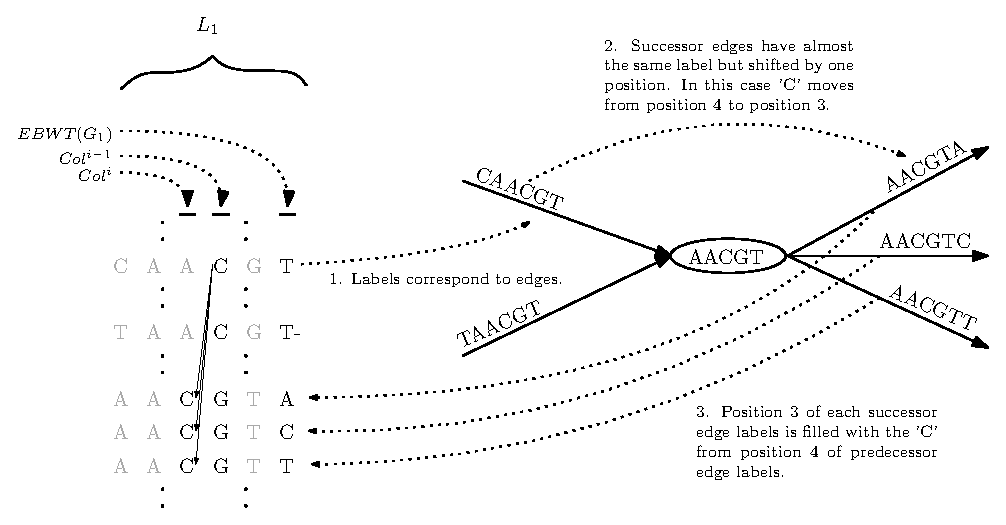
\includegraphics[width=1.0\textwidth]{varimerge/content/get_col.eps}
  	\caption{{\bf Method for populating $Col^i$ based on $Col^{i-1}$ and graph navigation.} Black nucleotides represent data that is in memory and valid.  Grey represents data that is stored in external memory in $\vari$ but is computed as needed and only exists ephemerally in $\ours$. Thus, only three columns are ever present in memory, which is a significant memory savings relative to the full set of edge labels.  The three resident vectors are 1.) $EBWT(G_1)$ (which is always present and used for navigation), 2.) $Col^{i-1}$ which is already completely populated when a new column to the left, 3.) ($Col^i$) is being generated.}

	\label{figure:get_col}
	
\end{figure}



Thus, we partition $P_1$ by first computing the subvector of $Col_1^i$ that is covered by $P_1[n]$, which we denote as $Col_1^i(P_1[n])$, and computing the subvector of $Col_2^i$ that is covered by $P_2[n]$, which we denote  as $Col_2^i(P_2[n])$.  Next, given a character $c$ in $\{ {\tt \$},  {\tt A}, {\tt C}, {\tt G}, {\tt T} \}$, we populate $SubP_1[c]$ and $SubP_2[c]$ based on $Col_1^i(P_1[n])$ {\em and} $Col_2^i(P_2[n])$ as follows: (1) we check whether $c$ exists in either $Col_1^i(P_1[n])$ or $Col_2^i(P_1[n])$; (2) if so, we add an interval to $SubP_1[c]$ covering the contiguous range of $c$ in  $Col_1^i(P_1[n])$ (or add an empty interval if $Col_1^i(P_1[n])$ lacks any instances of $c$), and add an interval to $SubP_2[c]$ covering the contiguous range of $c$ in  $Col_2^i(P_1[n])$ (or, likewise, add an empty interval if $Col_2^i(P_1[n])$ lacks any instances of $c$)\footnote{We are guaranteed by the definition of our data structure that any instances of $c$ in $Col_1^i(P_1[n])$ will be in a contiguous range, and likewise, any instances of $c$ in $Col_2^i(P_1[n])$ will also be in a contiguous range}.  Finally, we concatenate all the lists in $SubP_1$ and $SubP_2$ to form the revised plan $P_1'$ and $P_2'$. This revised plan $P_1'$ and $P_2'$ becomes the input $P_1$ and $P_2$ for the next refinement step. We refer the reader to Figure~\ref{alg:mergeexecute} in the supplement for the pseudocode. We crafted the method above to maintain the property described in the following observation.

\begin{observation} \label{obs} Let $P_1$ be a (partial) merge plan, and $P_1'$ its refinement by our merge algorithm, where $\ell_1,..,\ell_n$ are the elements in $\L_1$ that are covered by interval $p_{i} \in P_1$ and $m_1,...,m_o$ are the  elements of $\L_2$ covered by interval $q_{j} \in P_2$.  The following conditions hold:  (1) $|P_1| = |P_2|$ and $|P_1'| = |P_2'|$; (2) given any pair of
elements where $\ell_a \in p_i$, $\ell_b \in p_j$ and $p_i \cap p_j = \emptyset$ there exists intervals $p_i'$ and $p_j'$ in $P_1'$ such that  $p_i' \cap p_j' = \emptyset$ and  $\ell_a \in p_i'$, $\ell_b \in p_j'$; and lastly, (3) given an interval $p_i$ in $P_1$ and the subsets of the alphabet used $\sigma_1 \in \ell_1,..,\ell_n$ and $\sigma_2 \in m_1,...,m_o$, then $p_i$ will be partitioned into $|SubP_1| = |\sigma_1\cup\sigma_2|$ subintervals in $P_1'$.
\end{observation}

We defined this observation for $P_1$ but note that an analogous observation exists for $P_2$.








\subsubsection{The Execution Step.}

We execute the merge plan by combining the elements of $\EBWT(G)_1$ that are covered by an interval in $P_1$ with the elements of $\EBWT(G)_2$ that are covered by the equal position interval in $P_2$ into a single element in $\EBWT(G)_M$.  We note that when all characters of each label in $\L_{1}$ and $\L_{2}$ have been computed and accounted for, each interval in $P_1$ and $P_2$ will cover either 0 or 1 element of $\L_{1}$ and $\L_{2}$ and the number of intervals in $P_1$ (equivalently $P_2$) will be equal to $|\EBWT(G)_M|$. Thus, we consider and merge each pair of intervals of $P_1$ and $P_2$ in an iterative manner.  We let  $(p_i^1, p_i^2)$ as the $i$-th pair of intervals.  We concatenate the next character of $\EBWT(G)_1$ onto the end of $\EBWT(G)_M$ if $|p_i^1| = 1$.  If $|p_i^2| = 1$ then we dismiss the next character of  $\EBWT(G)_2$ since it is an abbreviated form of an identical edge to that just added. Next, if $|p_i^1| = 0$ and $|p_i^2| = 1$, we copy the next character from $\EBWT(G)_2$ onto the end of $\EBWT(G)_M$.  We refer the reader to Figure~\ref{alg:mergeexecute} for the pseudocode in the supplement.

We merge the color matrices in an identical manner by copying elements of $\C_1$ and $\C_2$ to $\C_M$.  Again, we iterate through the plan by considering each pair of intervals. If $|p_i^1| = 1$ and $|p_i^2| = 1$ then we concatenate the corresponding rows of $\C_1$ and $\C_2$ to form a new row that is added to $\C_M$.  If only one of $p_i^1$ or $p_i^2 $ is non-zero then the corresponding row of $\C_1$ or $\C_2$ is copied to $\C_M$ with the other elements of the new row set to $0$.


\subsubsection{Computational Complexity}

The following theorem demonstrates the efficiency of our approach.

\begin{theorem} Given two de Bruijn graphs $G_1 = (V_1, E_2)$ and $G_2 = (V_2, E_2)$ constructed with integral value $k$ such that, without loss of generality, $|E_1| \geq |E_2|$, it follows that our merge algorithm constructs the merged de Bruijn graph $G_M$ in $\bigO(m \cdot \max(k, t))$-time, where $t$ is the number of colors (columns) in $\C_M$ and $m = |E_1|$. \end{theorem}

\begin{proof}     In our merge algorithm, we will perform $k$ refinements of $P_1$ and $P_2$ after they are initialized. We know by definition and Observation \ref{obs} that $|P_1| \leq |\L_1|$,  $P_2 \leq |\L_2|$, $Col_1^i \leq |\L_1|$ and $Col_2^i \leq |\L_2|$ at each iteration $i$ of the algorithm.  Further, it follows from Observation \ref{obs} that a constant number of operations are performed to $P_1$,  $P_2$, $Col_1^i$ and $Col_2^i$. We populate $\C_M$ in the last step of merging the primary components of the data structure.  Since the  $\C_M$ is a bit matrix of size $k$ by $t$, it follows that this step will take time $\bigO(m \max(k, t))$-time.  Hence, if $k \leq t$ the merge algorithm will take $\bigO(mk)$-time; otherwise it will take $\bigO(mt)$-time (since populating $\C_M$ will dominate in this case).
\end{proof}

\subsubsection{Details of Merge Plan}
                        \label{merge_plan}

                        We recall a couple artifacts about the $\vari$ data structure prior to describing how we compute $Col_1^i$ (and $Col_2^i$).  We first note that $Col_1^{i-1}$ contains the $(q + 1)$-th position of every edge label, and after computation, $Col_1^i$ will contain the $q$-th position of every edge label.  Hence, we consider the characters in the label from right to left (i.e. decreasing sort precedence).  Fortunately, we have the final character of each edge label stored in $\EBWT(G)_1$ to begin---and thus, we  start by computing the second to final character ($(k-1)$-th position) and consider the characters in the decremented position at each iteration.   Second, we note that given any edge $e_{pred} = (s_{pred}, t_{pred})$ in $G_1$ and the $(q + 1)$-th character $c$ of the label of $e_{pred}$, all outgoing edges of $t_{pred}$, say $e_{succ}^1,..,e_{succ}^n$, have $c$ in the $q$-th position of their edge labels. This follows from the fact that $G_1$ is an de Bruijn graph.   Thus, we can compute $e_{succ}^1,..,e_{succ}^n$  by first performing a query of rank of $e_{pred}$ ($r = \rank(e_{pred}, \EBWT(G)_1)$) in order to identify $t_{pred}$, and then determining the appropriate range in $\EBWT(G)_1$ in order to find all outgoing edges of $t_{pred}$.  Given that the edges are in colex order of their $k-1$ prefix, we know all outgoing edges of $t_{pred}$ will be in a contiguous range in $\EBWT(G)_1$ and in the same relative order as their immediate predecessor edges. We find this range in $\EBWT(G)_1$ by computing $\select(\rank(\D_1[\label(e_{pred})] + 1, \B_{L_1}) + r - 1, \B_{L_1}),  \select(\rank(\D_1[\label(e_{pred})] + 1, \B_{L_1}) + r, \B_{L_1})]$.  We  use both these facts in our computation of $Col_1^i$  (See Figure~\ref{figure:partition}).

\begin{figure}[h]
	\centering
	
	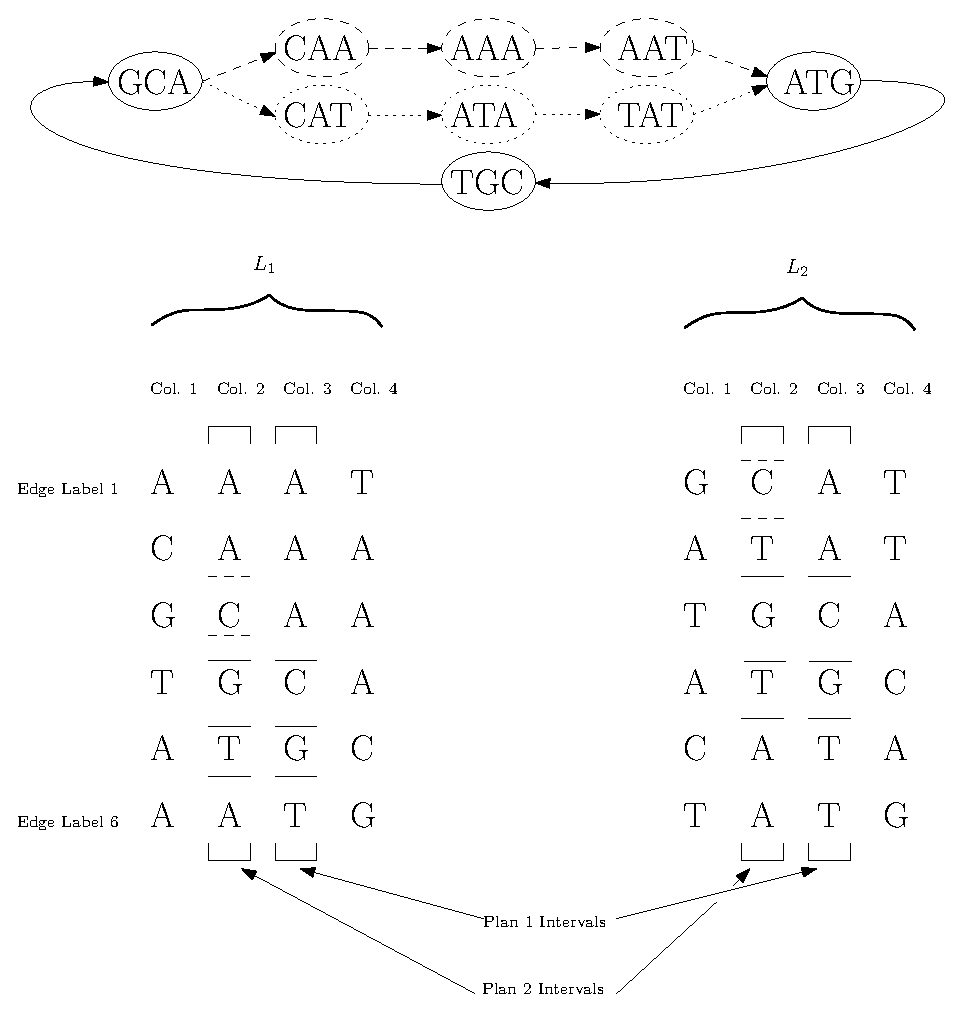
\includegraphics[width=.95\textwidth]{varimerge/content/partition.eps}
	\caption{{\bf Two lists of (conceptual) edge labels and the corresponding de Bruijn graph.} Dotted and dashed lines denote edges exclusive to one graph.  Solid lines are common to both.  The merged graph will contain all components.  Plans are refined in decreasing sort precedence order: (Col. 3, Col. 2,. Col. 1, Col. 4).  Plan 1 partitions the full range of edges into four intervals.  These intervals are further partition in Plan 2. The number of subintervals an interval is partitioned into depends on the size of the alphabet in use in both sub columns from $L_1$ and $L_2$ (e.g. The first interval in the $L_1$ half of Plan 1 is further partitioned into three sub intervals in Plan 2 (for `A', `C', and an empty one for `T') because the first interval in the $L_2$ half of Plan 1 has a `T').  This may introduce empty intervals, denoting that the corresponding edge labels for one graph are absent in the other.  Identical edge labels between graphs will always be in equal ranked intervals.  For example,  TCGA is in the second interval for both graphs in Plan 1, while it is in the fourth interval in Plan 2.}
	\label{figure:partition}
	
	
\end{figure}
                        

We define the computation of $Col_1^i$  by describing the following three cases.  When $1 < i < k$, we compute $Col_1^i$ by traversing $G_1$ in a forward direction from the first incoming edge of every node and copying the character found at the $(q + 1)$-th position of that incoming edge (again, stored in $Col_1^{i-1}$) into $q$-th position of all outgoing edges of that node.  When $i = 1$, the $(q+1)$-th position corresponds to $\EBWT(G)_1$, so $\EBWT(G)_1$ is used in place of $Col_1^{i-1}$ but is otherwise identical to the previous case.  Lastly, when $i=k$, we let $Col_1^i$ equal $\EBWT(G)_1$.


Here, we present our method for generating the secondary components of the succinct data structure for $G_M$.

\subsubsection{Delimiting common origin with $\B_{LM}$.}
We prepare to produce $\B_{LM}$ in the planning step by preserving a copy of the merge plan after $k-1$ refinement iterations as $S_{k-1}$. After $k-1$ refinement steps, our plan will demarcate a pair of edge sets where their labels have identical $k-1$ prefixes.  Thus, whichever merged elements in $\EBWT(G)_M$ result from those demarcated edges will also share the same $k-1$ prefix. Therefore, while executing the primary merge plan, we also consider the elements covered by $S_{k-1}$ concurrently, advancing a pointer into $\EBWT(G)_1$ or $\EBWT(G)_2$ every time we merge elements from them. We form $\B_{LM}$ by appending a delimiting 1 to $\B_{LM}$ (again, indicating the final edge originating at a node) whenever both pointers reach the end of an equal rank pair of intervals in $S_{k-1}$'s lists.
\subsubsection{Delimiting common destination with $\flags_M$.}
We produce $\flags$ in a similar fashion to $\B_{LM}$ but create a temporary copy of $S_{k-2}$ in the planning stage after $k-2$ refinement iterations instead of $k-1$.  In this cases, the demarcated edges are not strictly those that share the same destination; only those edges that are demarcated and share the same final symbol.  Thus, in addition to keeping pointers into $\EBWT(G)_1$ or $\EBWT(G)_2$, we also maintain a vector of counters which contain the number of characters for each (final) symbol that have been emitted in the output. We reset all counters to $0$ when  a pair of delimiters in $S_{k-2}$  is encountered.  Then, when we append a symbol onto $\EBWT(G)_M$, we consult the counters to determine if it is the first edge in the demarcated range to end in that symbol.   If so, we will not output a flag for the output symbol; otherwise, we will.

\subsubsection{Enabling navigation with $\D_M$.}

We produce $\D_M$ using the merge plan after the first refinement iteration.  The intervals at this point are identical to that encoded in $\D_1$ and $\D_2$ so we use the latter rather than consume more space with another copy of an intermediate merge plan.  Then, like for $\B_L$ we increment a variable tracking position within the intervals in parallel with consuming elements from $\EBWT(G)_1$ or $\EBWT(G)_2$. We count the number of emitted characters while consuming elements from each of the $\leq\sigma$ intervals and emit a prefix sum of these counts as $\D_M$.
































% \subsubsection{Figures Illustrating VariMerge.} We give two figures to illustrate the merge procedure of the primary components.  We show the planning stage in Figure \ref{figure:partition}, and how to produce the necessary components in memory in Figure \ref{figure:get_col}.














\renewcommand{\algorithmiccomment}[1]{\hskip0em$\triangleright$ #1}
\begin{figure}
%\begin{algorithm*}[h!t]
	
	\begin{algorithmic}
		\Procedure{Partition}{$W_1$,$W_2$}
		\State $\Sigma' \leftarrow \emph{AlphabetUsed}(W_1,W_2)$
		\State $SubP_1 \leftarrow ()$
		\State $SubP_2 \leftarrow ()$
		\ForAll{$c \in \Sigma'$}
		\State $SubP_1.\emph{Append}(\emph{IntervalOccupied}(c, W_1))$
		\State $SubP_2.\emph{Append}(\emph{IntervalOccupied}(c, W_2))$
		\EndFor
		\State \Return $(SubP_1, SubP_2)$
		\EndProcedure
		
		\\
		\Procedure{RefinePlan}{$P_1$, $P_2$, $Col_1$, $Col_2$, $i$}
		\State $P_1' \leftarrow ()$
		\State $P_2' \leftarrow ()$
		\State \Comment{For each interval in the (equal length) plans...}
		\ForAll{$j \in \{1..|P_1|\}$}
		\State \Comment{...extract a window from each column covered by the interval...}
		\State $W_1 \leftarrow \emph{CoveredSymbols}(Col_1, P_1[j])$
		\State $W_2 \leftarrow \emph{CoveredSymbols}(Col_2, P_2[j])$
		\State \Comment{...and partitioning that window on its character runs, forming sub-intervals.}
		\State $(SubP_1, SubP_2) \leftarrow \emph{Partition}(W_1, W_2)$
		\State $P_1'.\emph{Concatenate}(SubP_1)$
		\State $P_2'.\emph{Concatenate}(SubP_2)$
		\EndFor
		\State \Comment{Capture snapshots of important intermediate plan states.}
		\If {$i \in \{1, k-1, k-2\}$ }
		\State $S_{i} \leftarrow (P_1', P_2')$
		\EndIf
		\State \Return $(P_1', P_2')$
		\EndProcedure
		\\
		\Procedure{VariMergePlan}{$G_1$, $G_2$}
		\State \Comment{Initialize plan to single intervals covering entire $EBWT(G)$s.}
		
		\State $P_1 \leftarrow ([1, |EBWT(G)_1|])$
		\State $P_2 \leftarrow ([1, |EBWT(G)_2|])$
		
		\State \Comment{Iterate through ``edge label matrix'' columns in sort precedence order}
		\ForAll{$i \in \{1..k\}$}
		\State $Col_1 \leftarrow \emph{GetCol}(i, G_1)$
		\State $Col_2 \leftarrow \emph{GetCol}(i, G_2)$
		
		\State $(P_1', P_2') \leftarrow \emph{RefinePlan}(P_1, P_2, Col_1, Col_2, i)$
		\State $(P_1, P_2) \leftarrow (P_1', P_2')$
		\EndFor
		\EndProcedure
	\end{algorithmic}
	
%\end{algorithm*}
	\caption{Algorithm to generate a plan.  \emph{AlphabetUsed}() returns the set of symbols used in its arguments. \emph{IntervalOccupied}() returns the $c$ run interval found in its second window argument. Assume window objects ($W_1$ and $W_2$) retain their origin such that \emph{IntervalOccupied}() returns intervals with respect to the source positions in $Col_1$ and $Col_2$. \emph{CoveredSymbols}() returns the substring (with the aforementioned source interval) which is covered by an argument interval. \emph{IntervalLast}() returns true if the given position is the last in the given interval.  For completeness we give all the pseudocode, including that given in the main paper.} \label{alg:mergeplan2}
\end{figure}

\begin{figure}
%\begin{algorithm*}[t]


	
	\begin{algorithmic}
		
		\Procedure{VariMergeExecute}{$G_1$, $G_2$}
		\State \Comment{Phase 2: Execute plan}
		\State \Comment{For each interval in the (equal length) plans...}
		\ForAll{$j \in \{1..|P_1|\}$}
		\State $NTcounts \leftarrow [0,0,0,0,0]$
		\State $flagcounts \leftarrow [0,0,0,0,0]$
		\State $EBWT(G)_M \leftarrow (), B_{LM} \leftarrow (), flags_M \leftarrow ()$
		\State $G1ptr \leftarrow 1, G2ptr \leftarrow 1$
		\If {$|P_1[j]| = 1$}
		\State $EBWT(G)_M.\emph{Append}(EBWT(G)_1[G1ptr]$)
		\State $B_{LM}.\emph{Append}(\emph{IntervalLast}(G1ptr, S_{k-1}[1]))$
		\State $flags_M.\emph{Append}(flagcounts[EBWT(G)_1[G1ptr]] \neq 0)$
		\State $flagcounts[EBWT(G)_1[G1ptr]] \leftarrow +1$
		\State $G1ptr \leftarrow +1$
		\If {$|P_2[j]| = 1$}
		\State $G2ptr \leftarrow +1$
		\EndIf
		\Else
		\State $EBWT(G)_M.\emph{Append}(EBWT(G)_2[G2ptr]$)
		\State $B_{LM}.\emph{Append}(\emph{IntervalLast}(G2ptr, S_{k-1}[2]))$
		\State $flags_M.\emph{Append}(flagcounts[EBWT(G)_2[G2ptr]] \neq 0)$
		\State $flagcounts[EBWT(G)_2[G1ptr]] \leftarrow +1$
		\State $G2ptr \leftarrow +1$
		\EndIf
		\State \Comment{When the last symbol(s) are consumed from equal an rank interval pair in $S_{k-2}$, reset the flag counter.}
		\If {$\emph{IntervalLast}(G1ptr, S_{k-2}[1]) \bf{and} \emph{IntervalLast}(G2ptr, S_{k-2}[2])$}
		\State $flagcounts \leftarrow [0,0,0,0,0]$
		\EndIf
		\EndFor
		\State $D_M \leftarrow \emph{PrefixSum}(NTcounts)$
		\EndProcedure
		
      \end{algorithmic}
      \caption{Algorithm to execute the merge plan.}
      \label{alg:mergeexecute}
%\end{algorithm*}
\end{figure}









\subsection{Discussion}

In this section, we present our experimental results on {\em E. coli} and GenomeTrakr data. We show the scalability of $\ours$ by demonstrating the time and computational resources needed to build the colored de Bruijn graph for 16,000 strains of salmonella.  Next, in order to validate the correctness of our approach, we generated two succinct colored de Bruijn graphs with sets of three  \emph{E. coli} assemblies each, merged them, and verified its equivalence to a six color graph built from scratch.  This experiment demonstrates that the merged colored de Bruijn graph is equivalent to that produced by building the graph without merging.    We ran all performance experiments on a machine with two Xeon E5-2640 v4 chips, each having 10 2.4 GHz cores.  The system contains 755 GB of RAM and two ZFS RAID pools of 9 disk each for storage.  We report wall clock time and maximum resident set size from Linux.  We use the SDSL-Lite library~\cite{SDSL} to store all succinct vectors.

\begin{sidewayspage}
  
    \begin{table}[h!]
%        \vspace{-10mm}
%      \vspace{-5mm}
    \caption{Comparison between building a succinct colored de Bruijn for the same 8,000 Salmonella strains using $\vari$ versus $\ours$.}
%\fontsize{2mm}{2mm}\selectfont
  \begin{center}
      \resizebox{8in}{!}{
\begin{tabular}{|l|r|r|r|r|r|r|r|r|r|r|r|r|}
\hline
&  \multicolumn{2}{|c|}{Input Stats} & \multicolumn{3}{|c|}{de Bruijn Graph } & \multicolumn{3}{|c|}{Color Matrix } & \multicolumn{4}{|c|}{Combined Requirements}\\
\hline
\textbf{Program and Dataset} & \textbf{$k$-mers} & \textbf{Colors} & \textbf{ RAM}& \textbf{Time} & \textbf{Size} & \textbf{RAM} &   \textbf{Time} & \textbf{Size} &  \textbf{RAM}  & \textbf{Ext. Mem.}  &   \textbf{Time} & \textbf{Size} \\
\hline
$\vari$(8k-1)   & 2.4 B       & 8,000 &              271 GB      & 30 h 49 m & 0.63 GB &              117 GB     & 6 h 28 m   & 114 GB              &    271 GB  & 4.6 TB  & 37 h  27 m &  114 GB \\
$\ours$(8k-1)      & 2.4 B     & 8,000 &              137 GB      & 21 h 27 m & 0.63 GB &              117 GB    & 5 h 3 m    & 114 GB               &    137 GB  & 1.5 TB  & 26 h  30 m & 114 GB\\
\hline

\end{tabular}
}
  \label{tab:compare}
\end{center}
\end{table}
\begin{table}[h!]
%    \vspace{-10mm}
  \caption{Breakdown of the components of $\ours$ which was listed in the table above. }%The $\ours$ method consists of running $\vari$ on subsets of the population (4k-1 and 4k-2) and then merging the results with our proposed merge algorithm (denoted $\merge$ here).}
  % Here we list the resources used for both individual runs of VARI as well as the merge.  We also list the combined resources, consisting of the total time and maximum space used across all three components of $\ours$ used in this dataset.
%Both $\vari$ and our merge algorithm each consist of two programs: one primarily responsible for the succinct de Bruijn graph and one for compressing the color matrix.  The resources for these are listed in separate columns and the combined resources needed for each method in the rightmost columns.  Size is the resulting succinct data structure size.}
%\fontsize{2mm}{2mm}\selectfont
  \begin{center}
      \resizebox{8in}{!}{
\begin{tabular}{|r|r|r|r|r|r|r|r|r|r|r|r|r|}
\hline
&  \multicolumn{2}{|c|}{Input Stats} & \multicolumn{3}{|c|}{de Bruijn Graph } & \multicolumn{3}{|c|}{Color Matrix } & \multicolumn{4}{|c|}{Combined Requirements}\\
\hline
\textbf{Program and Dataset} & \textbf{$k$-mers} & \textbf{Colors} & \textbf{ RAM}& \textbf{Time} & \textbf{Size} & \textbf{RAM} &   \textbf{Time} & \textbf{Size} &  \textbf{RAM}  & \textbf{Ext. Mem.}  &   \textbf{Time} & \textbf{Size} \\
\hline
$\vari$(4k-1)      & 1.1 B    & 4,000 &               136 GB      & 8 h 46 m  & 0.31 GB &              52 GB     & 1 h 39 m & 51.2 GB               & 136 GB & 1 TB    & 10 h 25 m & 51 GB \\
$\vari$(4k-2)      & 1.5 B    & 4,000 &              137 GB      & 10 h 40 m & 0.52 GB &              54 GB     & 2 h 22 m & 52.5 GB                &  137 GB & 1.5 TB  &  13 h  2 m & 53 GB\\
$\merge$(4k-1, 4k-2)  & 2.4 B    & 8,000 &              10 GB       & 2 h 1 m   & 0.63 GB &              117 GB    & 1 h  2 m & 106 GB               &  117 GB    &  N/A    &  3 h 3 m & 106 GB \\
\hline
$\ours$(8k-1)      & 2.4      & 8,000 &              137 GB      & 21 h 27 m & 0.63 GB &              117 GB    & 5 h 3 m  & 117 GB               &    137 GB  & 1.5 TB  & 26 h  30 m & 106 GB\\
\hline
\end{tabular}
}
\label{tab:breakdown}
\end{center}
\end{table}
%\end{sidewayspage}
%\begin{sidewayspage}
\begin{table}[h!]
%    \vspace{-10mm}
  \caption{Additional statistics for building a Salmonella 16,000 strain succinct colored de Bruijn graph.}% ({\it n.b.} $\ours$ includes the resources required of the two 4k runs of VARI and the 8k run of $\ours$ from Table 2.}
%\fontsize{2mm}{2mm}\selectfont
  \begin{center}
      \resizebox{8in}{!}{
\begin{tabular}{|l|r|r|r|r|r|r|r|r|r|r|r|r|}
\hline
&  \multicolumn{2}{|c|}{Input Stats} & \multicolumn{3}{|c|}{de Bruijn Graph} & \multicolumn{3}{|c|}{Color Matrix} & \multicolumn{4}{|c|}{Combined Requirements}\\
\hline
\textbf{Program and Dataset} & \textbf{$k$-mers} & \textbf{Colors} & \textbf{ RAM}& \textbf{Time} & \textbf{Size} & \textbf{RAM} &   \textbf{Time} & \textbf{Size} &  \textbf{RAM}  & \textbf{Ext. Mem.}  &   \textbf{Time} & \textbf{Size} \\
\hline
$\vari$(4k-3)       & 1.7 B    &  4,000 &              135 GB      & 10 h 53 m & 0.46 GB &              53 GB     & 2 h 34 m & 51.8 GB               & 135 GB & 1.6 TB  & 13  h  27 m     & 52 GB \\
$\vari$(4k-4)       & 2.4 B    &  4,000 &              137 GB      & 14 h 35 m & 0.67 GB &              59 GB     & 3 h 37 m & 57.9 GB               & 137 GB & 2.34 TB & 18 h   12 m         & 59 GB\\
$\merge$(4k-3, 4k-4)   & 3.8 B    & 8,000  &              17 GB       & 2 h 59 m  & 1.00 GB &              118 GB    &  57 m    & 107 GB                &  118 GB & N/A     &     3 h 56 m             & 108 GB \\
$\merge$(8k-1, 8k-2)   &   5.8 B & 16,000 &               25 GB       & 4 h 53 m  & 1.60 GB &              254 GB    & 2 h 10 m & 232 GB                &  254 GB & N/A     &     7 h 3 m            & 233 GB \\
\hline
$\ours$(16k)        &  5.8 B  & 16,000        &         137 GB     & 54 h 47 m    &  1.60 GB &                254 GB   &   14 h 21 m       &       232 GB      &    254 GB & 2.34 TB &       69 h 8 m           &  233 GB \\
\hline
\end{tabular}
}
\label{tab:build}
\end{center}
\end{table}
\end{sidewayspage}

\subsubsection{Large-scale Construction using GenomeTrakr}

We demonstrate the scalability of $\ours$ by constructing the succinct  de Bruijn graph for 16,000
Salmonella strains from  NCBI BioProject PRJNA183844. We downloaded the sequence data from NCBI and preprocessed the data by assembling each individual sample with IDBA-UD  and counting  $k$-mers ($k$=32) using KMC.  We used these $k$-mers as input to $\ours$.  We modified IDBA by setting kMaxShortSequence to 1,024 per public advice from the author to accommodate the longer paired end reads that modern sequencers produce.  We sorted the full set of samples by the size of their $k$-mer counts and selected 16,000 samples about the median.  This avoids exceptionally short assemblies, which may be due to low read coverage, and exceptionally long assemblies which may be due to contamination.  We divide these 16,000 samples into four sets of 4,000 which we label 4k-1, 4k-2, 4k-3, and 4k-4. The exact accessions for each dataset is available in our repository. Merged graphs are numbered in the order of their constituents (e.g. the merged 8k-1 comprises the graphs from 4k-1 and 4k-2.)   We summarize our results in Table 1.

In order to measure the effectiveness of $\ours$ for incremental additions to a graph that holds a growing population of genomes, we constructed the colored de Bruijn graph using $\vari$ for a set of 4,000 salmonella assemblies (4k-1) as well as for a set of just one assembly.  Next, we ran our proposed merge algorithm on these two graphs.  $\vari$ took 8 hours 46 minutes, 1 TB of external memory, and 136 GB of RAM to build the graph for 4,000 strains.  To build a single colored de Bruijn graph for an additional strain, $\vari$ took 27 seconds, 10 GB of external memory, and 3 GB of RAM.  Our proposed  algorithm took 49 minutes, no external memory, and 5 GB of RAM to merge the 4,000 color graph with the 1 color graph. This is considerably faster than it would take to build a 4,001 color graph from scratch.
In order to measure the effectiveness of $\ours$ for the proposed divide-and-conquer method of building large graphs, we built a graph for a second set of 4,000 assemblies (4k-2) using 10 hours 40 minutes, 1.5 TB of external memory, and 137 GB of RAM.  We merged these two 4,000 sample graphs (i.e. 8k-1) using our proposed algorithm in 2 hours 1 minutes, no external memory, and 10 GB of RAM.  Thus the $\ours$ method required a combined 137 GB of RAM, 26 hours 30 minutes of runtime to produce the 8k-1 graph.   In contrast, running $\vari$ on the same 8,000 strains (8k-1) required 37 hours 27 minutes, 4.6 TB of external memory and 271 GB of RAM. Thus $\ours$ reduced runtime by 11 hours, reducing RAM requirements to 134 GB, and reducing external memory requirements by 3.1 TB.

We further used this facility to merge two more 4,000 color graphs (i.e. 4k-3 + 4k-4 = 8k-2) and then merged this 8,000 sample graph with the aforementioned 8,000 graph to produce a succinct colored de Bruijn graph of 16,000 samples (i.e. 8k-1 + 8k-2 = 16k-1).

















\begin{figure}[h!t]
%  \parbox{0.45\textwidth}{
  %}
  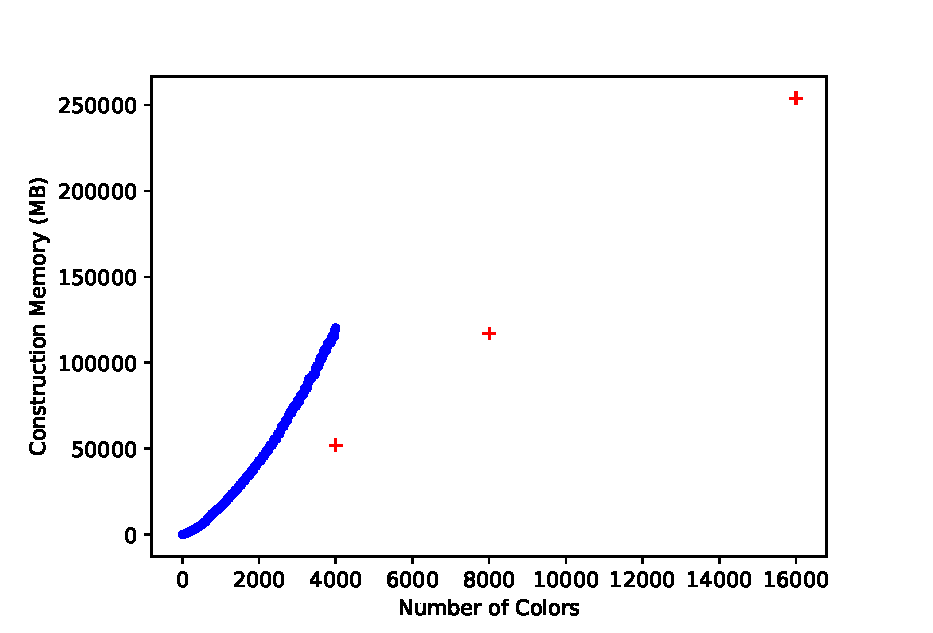
\includegraphics[width=1.0\textwidth]{varimerge/content/BFTvsVARI.eps}
    \caption{Comparison between Bloom Filter Trie (blue dots) and $\ours$ (red pluses) on isolates from GenomeTrakr.  We ran Bloom Filter Trie on 4,000 isolates and plot $\ours$ results up through 16,000 isolates.}

\label{fig:bftvsvari}
\end{figure}


\subsubsection{Comparison to Bloom Filter Trie}

In addition to demonstrating scalability, we used the Samonella strains from GenomeTrakr to directly compare the data structure space and construction memory of $\ours$ with Bloom Filter Trie~\cite{holley2015bloom} (BFT).  We observe both tools have a small memory overhead in construction above the final data structure. We found super-linear growth in BFT construction memory
%(see Figure~\ref{fig:bftvsvari}),
%TODO fix broken fig:bftvsvari refs
and that BFT produced a graph 105 GB in size after 4,000 samples were inserted. This is only slightly less space than the 106 GB the $\vari$ data structure requires to represent twice as many samples.  Holley  et al.~\cite{holley2015bloom} report  sub-linear growth up through 471 samples; however, we posit these differing observations may be a result of both differing dataset and preprocessing methods; More specifically, these isolates were extracted from a single species (humans) in contrast to GenomeTrakr, and thus may result in data that is more more homogeneous and has slower growth in the diversity with population size;  GenomeTrakr Salmonella samples are culled from  diverse food production environments.  Furthermore, they filter $k$-mers that have low multiplicity as a means to clean the data. This may reduce the growth as parts of the so called core genome may be missing in some samples, and the set of population $k$-mers could converge asymptotically toward the core genome.  Though Holley {\it et al.} compared to Sequence Bloom Trees by Solomon {\it et al.}~\cite{solomon2015large}, we do not because the Sequence Bloom Tree software is designed for transcript querying rather than variant detection.
















\subsubsection{Validation using E. coli}


We validate $\ours$ by generating two succinct colored de Bruijn graphs with three \emph{E. coli} assemblies each, merge them, and verify correctness of the merged graph:    First, we generated all $k$-mers for each reference genome, counted all unique $k$-mers with KMC2~\cite{deorowicz2015kmc}, constructed two de Bruijn graphs of three assemblies each using $\vari$, and merged them into a six color graph using $\ours$.  Independently, we constructed a second colored de Bruijn graph using $\vari$ on all six assemblies in one run, and compared these two graphs.  We found $\ours$ produced files on disk that were bit-for-bit identical to those generated by $\vari$, demonstrating they construct equivalent graphs and data structures.






\subsection{Conclusions}


In this section, we propose to further increase the scalability of succinct colored de Bruijn graphs by developing a method to merging smaller graphs in a resource-efficient manner.  This allows the colored de Bruijn graph to be constructed for massive size datasets.  In addition, our algorithm provides an efficient means to update a succinct colored de Bruijn graph with additional data  as it becomes available. This is useful for example, in the GenomeTrakr database, which is continually being updated with more data on a monthly (or even weekily basis) and the search for a foodborne outbreak requires the analysis of the complete dataset.  Thus, rather than rebuilding the colored de Bruijn graph on the new (complete) version of the GenomeTrakr data, dynamically updating the existing one  would ensure ideal use of time and resources.

Lastly, our merge algorithm may be applicable to  to other prefix-only compressed suffix arrays such as GCSA by Sir{\'e}n {\it et al.}~\cite{siren2014indexing} and XBW by Ferragina {\it et al.}\cite{ferragina2009compressing}.  This merits future investigation as these data structures are of both theoretical and practical interest.

























\chapter{Conclusion}
\bigskip

In this work we've seen that the FM-Index can be usefully applied to various genomics problems.  Both $\twin$ and $\dopp$ exploit the FM-Index's ability to find all matches in the target data concurrently as opposed to exhaustively searching all regions of the target data serially.  Both $\vari$ and $\ours$ exploit the compressed nature of the FM-Index to reduce memory consumption.  

As both $\dopp$ and $\vari$ represent graphs of many sequences (Rmaps and samples, respectively) it is useful to consider how they differ, and if each data structure would have a useful application in the  domain where we've seen the other used.  First, we should consider the several notable differences between these structures the impact their application.  In the succinct colored de Bruijn graph, common substrings between two samples give rise to $(k-1)-mers$ glued together and any differing regions give rise to bubbles in the graph.  Thus the glued $(k-1)-mers$ are effectively seed matches in an alignment and traversal of the graph reveals the mismatching regions containing insertions, deletions, or substitutions.  These alignments are found entirely within the data structure after construction and can thus take the form of many-to-many alignments. In contrast, in the GCSA we find alignments between a single query sequence which is not part of the data structure and all compatible matches within the data structure are found concurrently, thus representing a one-to-many alignment.  

We might also consider how repeats in the underlying data are handled differently by the two structures.  As previously discussed, an important construction step of GCSA is inducing the prefix sortedness property, such that vertices form a totally ordered set based on the lexicographic rank of their corresponding suffix set. Repeats introduce suffixes that may  have identical prefixes interfering with total ordering. Thus, the more repeats that are present in a dataset, the more work must occur during construction of a GCSA structure (i.e. prefix doubling enough for unambiguous lexicographic order) and the resulting structure may consequently be larger.  We can also consider each vertex in a de Bruijn graph as representing a suffix in a set of spellable strings, but always just the $k$ length prefix of those strings.  As such, in contrast, in the succinct colored de Bruijn graph, all repeated regions longer than $k$ in length result in a collection of single vertices, each with a unique label.  So since all vertices are unique, they always have a total order. In essence, the succinct colored de Bruijn graph deals with repeats by collapsing all instances to a single $k$-length string and keeping track of their origin in the color matrix.   In contrast, GCSA deals with repeats by keeping separate vertices for each copy of a repeat, at the expense of expanding the size of the graph to induce a total order. 

Given this, we might consider scenarios where we allow gluing of similar fixed length segments of the $\dopp$ graph and keeping track of the origin Rmaps in a color matrix.  Under such a scenario, we would also have to consider the sizing error problem. However, the notion of speculating error could be extended to quantization, where additional vertices are introduced to capture the possibility a given Rmap fragment's true size would yield an adjacent quantization bin.  The complementary application, finding sequence alignments to sets of finished genomes is already embodied in the original GCSA work.

Future work could include further compressing the color matrix by marking which color matrix rows are identical to their predecessor in compressible runs in the graph, thus obviating the need to store any `1' bits for those rows.  This would be akin to colored compact de Bruijn graphs which need only associate one set of colors with a compacted node instead of with each of the non-compacted nodes it comprises.

As well, the colored de Bruijn graph could be made variable order (in concert with the work of Boucher {\it et al.}~\cite{boucher2015variable} by orienting the color matrix in column major order.  If the suggested radix merge method is further developed, it could potentially be used to generate the required LCP array in a variable order succinct colored de Bruijn Graph.

Additionally, one of the key features that made the FM-Index techniques work for optical mapping is that the errors in the data were constrained about the given data -- sizing error was always distributed about the true size and missing sites could be speculated about.  This suggests this same technique could be applied to other data sources, such as sequencing platforms that are error prone in the length homopolymer runs, which could be indexed  as run lengths stored in a wavelet tree.




% TODO CHUCK Can you add some indications of success and respect from community, other than publications? How many times has your software been downloaded? What well known labs are using your methods?

% TWIN google analytics page view for download page count UA-35939827-1 for TWIN
% UA-56055810-1 for misSEQuel









\input{postamble}
